\documentclass[10pt,a4paper]{article}
\usepackage{geometry}%—— 宏设置页边距
\geometry{left=2.5cm,right=2.5cm,top=2.5cm,bottom=2.5cm}
\usepackage{amsmath}%—— 数学
 \usepackage{amssymb}%—— 数学
 \usepackage{amsthm}
 \usepackage{graphicx}%—— 插图
 \usepackage{array}%—— 表格文字居中
\usepackage{microtype}%改善了单词、字母的间距
\usepackage{listings}%代码宏
\usepackage[normalem]{ulem} % use normalem to protect \emph
\newcommand\hl{\bgroup\markoverwith
  {\textcolor{lightgray}{\rule[-.5ex]{.1pt}{2.5ex}}}\ULon}
\usepackage{algpseudocode}
\usepackage[unicode,naturalnames]{hyperref}%——————————————————————目录超链接
%\usepackage{xcolor}%——————————————————————改变文字颜色

\usepackage[linesnumbered,ruled]{algorithm2e}
\usepackage{algorithmicx}
%\usepackage{pxfonts}
\usepackage{libertine}
\usepackage{libertinust1math}
\usepackage[T2A,T1]{fontenc}
\usepackage[utf8]{inputenc}
\usepackage[english,russian]{babel}
\linespread{1.0} %—— 行间距
\setlength{\parskip}{0em}%设置段落间距
\title{ \LARGE\bf PPIO: Программируемая одноранговая сеть\\хранения и доставки}  %———标题

\begin{document}
\maketitle%—— 显示标题
% \newpage 
\renewcommand{\baselinestretch}{1.2}
\author {\centerline{\Large Аннотация}}
\noindent\\
PPIO является программируемой децентрализованной сетью хранения и доставки данных. Она не только предоставляет более мощные и эффективные службы, нежели существующие облачные платформы хранения данных, такие как AWS S3, но, так же, значительно снижает стоимость хранения.  В то же время, PPIO предлагает лучшую защиту в аспектах безопасности и приватности. Грамотно продуманная распределенная сеть хранения и механизм поощрения позволяют PPIO использовать значительный объем неиспользованной полосы пропускания и ресурсы хранилищ в сети Интернет, а так же, предоставлять надежные услуги хранения с намного меньшей ценой. Уникальная децентрализованная файловая система PPIO предоствращает неавторизованный доступ и гарантирует безопасность и приватность хранения данных. PPIO спроектирована с нуля для эффективного функционирования в глобальном масштабе, на основании опыта команды разработчиков в проектировании и запуске децентрализованной сети с сотнями миллионов пользователей. PPIO сводит потребности в хранении данных, имеющиеся у сегодняшнего бизнеса с одной стороны и предлагаемых возможностей поставщиков соответствующих услуг с другой, а так же, предоставляет возможность реализации распределенных приложений (DApps).
\vspace{-0.5em}
\\ \\ В данном документе разъясняются основные цели архитектуры PPIO, а так же, приводятся подробности методов достижения этих целей. Документ предоставляет низкоуровневую подробную информацию о распределенной файловой системе, архитектуре сети и процесса хранения. Документ разъясняет как PPIO противостоит различным сетевым атакам, поддерживает работоспособность и устойчивость механизма поощрений, предлагает экономическую модельи экосистему.
\newpage
\tableofcontents %—— 制作目录(目录是根据标题自动生成的)
\newpage
\section{Введение} %—1
\vspace{-0.5em}
Глобальный рынок облачных хранилищ в значительной мере вырос за последние годы и продолжает расти быстрыми темпами . Тем не менее, существующие централизованные решения имеют множество проблем. Порча и утеря данных происходят все чаще, с постоянно растущим масштабом и влиянием. Например, в 2016 году был взломан Dropbox, что привело к утечке 68 миллионов пользовательстких аккаунтов. Такие инциденты представляют серьезную угрозу не только приватности отдельных пользователей, но, так же, безопасности и целостности всего Интернета. Так же, другой проблемой централизованных систем хранения является высокая стоимость каналов связи и хранилищ, она приводит к неприемлемой цене и делает крайне сложным прибыльность для многих Интернет-компаний.
\vspace{-0.5em}
\\ \\Предпринималось не мало попыток построения распределенных систем хранения данных. Тем не менее, эти попытки не были успешными. Одна из таких попыток, Seacoin, построенная на основе Бикоин-подобного консенсуса Proof of Work (PoW). PoW предполагает производство массивных вычислений, тем самым форсирует потребление большого количества энергии, а так же, он не учитывает объемы хранилищ и мощность каналов связи майнеров, являющихся ключевыми аспектами в децентрализованной распределенной системе хранения данных. Storj, другой проект, разрабатываемый вот уже в течении нескольких лет, но так и не вышедший из фазы тестирования. Некоторые из известных проблем Storj - это невозможность получения быстрого ответа от майнеров относительно запросов на хранение, а так же их транзакций, фиксируемых раз в месяц, что не является удобным для майнеров. BurstCoin использует Proof of Capacity (PoC), учитывающий размер хранилищ майнеров, но, к сожалению, этого не достаточно для нормального функционирования хранилища с выполнением всех требований к нему.
\vspace{-0.5em}
\\ \\Новый проект FileCoin, разрабатываемый Protocol Labs, добавляет слой поощрений над Inter-planetary File System (IPFS), с целью построения инфраструктуры хранилищ и протокола для замены HTTP. Для этой цели индекс файлов делается публичным, что создает возможности наподобие Веб-доступа к файлам, но это, так же, создает проблему сохранения приватности пользователя и безопасности данных в сети. Кроме того, некоторые из криптомеханизмы слишком сложны и предположительно будут негативно сказываться при большом масштабе системы. FileCoin использует архитектуру одноранговых сетей из проверенных временем приложений, таких как BitTorrent, но, не предоставляет решений для сложных сетевых сред и не предлагает скоростных оптимизаций для региональных сетей. Такие ущербности в заимствованной архитектуре могут приводить ко множеству проблем в реальном использовании, как для майнеров так и для поставщиков интернета (Internet Service Providers, ISPs). Как заявляет Protocol Labs, файлы, размещенные в IPFS являются перманентными, не могут быть удалены, что может приводить к юридическим битвам в аспекте государственных политик и регуляторов, глобальное распространение файлов становится намного более сложным.
\vspace{-0.5em}
\\ \\Из изложенного выше становится понятно, что готовая децентрализованная распределенная система хранения, способная поддерживать высокое масштабирование и задачи реального мира, еще не построена. Вот чего пытается достигнуть PPIO. Команда, учредившая и разрабатывающая PPIO успешно спроектировала, разработала и поддерживает PPLive, одноранговую систему вещания, обслуживающую сотни миллионов пользователей ежедневно. Такой опыт позволяет команде разрабатывать эффективное и практичное решение, направленное на следующие цели.
\vspace{-0.6em}
 \\ 
 
 \hangafter 1
\hangindent 1.5em
\noindent   
•\quad  {\bf Малая цена хранения.} В будущем, высокая цена хранения данных будет одним из критичных вызовов для многих компаний. Грамотно спроектированные поощрения в PPIO предоставляют привлекательные винансовые вознаграждения майнерам и провоцируют их на взаимодействие с сетью. В то же время, они наказывают неадекватных участников. В результате может быть сформировано большое и качественное сообщество майнеров. Это позволяет PPIO задействовать большое количество неиспользуемой полосы пропускания каналов связи и ресурсов хранилищ в сети Интернет, предоставить мощную услугу хранения данных по сильно менщей цене. Для облегчения использования системы хранения, PPIO предлагает схему, называемую "Coin Pool", помогающую пользователям выгружать и загружать микроплатежи. Так же, ахитектура PPIO включает механизм противостояния колебаниям цены хранения, предоставляющий пользователям лучший вариант чем существующие централизованные платформы хранения и, что не менее важно, по намного меньшей цене.
\vspace{-0.6em}
\\ \

\hangafter 1
\hangindent 1.5em
\noindent   
•\quad {\bf Масштабируемость и высокая эффективность.} За счет опыта команды, извлеченного из создания и работы с распределенной сетью с тысячами миллионов пользователей, PPIO спроектирована с нуля до состояния, в котором она может быть эффективной в глобальном масштабе. Наряду с множеством проверенных в промышленных условиях одноранговых технологий передачи, команда так же разработала планировщик, управляемый данными (data-driven scheduling), самоорганизующуюся оверлейную сеть и сеть оптимального распространения контента. Архитектура PPIO, так же, направлена на увеличение эффектирвности  работы в региональных сетях, что делает ее более дружелюбной к поставщикам интернета (ISP). Комбинируя свои иннвации с такими технологиями как обход NAT (NAT Traversal), распределенные хэш-таблицы (DHT) Kademlia, облегченное доказательство консенсуса хранилища и оптимизированное потоковое
вещание медиа, распределенная сеть хранения PPIO может быть крайне эффективной и может быть легко масштабирована на сотни миллионов сетевых узлов.
\vspace{-0.6em}
\\ \

\hangafter 1
\hangindent 1.5em
\noindent   
•\quad {\bf Приватность, безопасность и стабильность.} Безопасность и приватность данных являются ключевыми требованиями в дизайне распределенной файловой системе PPIO. За счет алгоритмов шардинга и шифрования, пользовательские данные могут быть получены только обладателем приватного ключа пользователя. В то же время, они позволяют пользователю делиться данными публично или в приватной группе. Для обеспечения целостности и доступности хранимого контента, PPIO снабжена практичными механизмами доказывания. Облегченное доказательство вместимости (Light Proof of Capacity, LPoC) разработано для легкого удостоверения в наличии заданного объема свободного места в распоряжении майнера. Оптимизированное доказательство хранения с течением времени (Оptimized Proof of Space-Time, PoSt) убеждает что заданные данные действительно сохранены майнером в течении периода времени. Доказательство пересылки (Proof of Replication, PoRep) гарантирует то что майнет реплицировал пользовательские данные. Доказательство получения (Proof of Download, PoD) убеждает пользователя в том что он может корректно получить хранимые майнером данные.
\vspace{-0.6em}
\\ 

\hangafter 1
\hangindent 1.5em
\noindent   
•\quad {\bf Надежная поддержка приложений и экосистема.} PPIO предоставляет несколько программных интерфейсов хранилищ (Storage APIs), похожих на таковые в облачных сервисах, например AWS S3, и позволяет комфортно мигрироать данные из этих сервисов. PPIO так же имеет некоторые технологии для улучшения поддержки распределенных приложений, включая хранилища объектов, механизм песочницы, управление доступом к файлам и т.п. PPIO имеет обстоятельный план для разработки сильной, живучей и устойчивой экосистемы для разработки приложений и сервисов, и предоставления разработчикам возможности наслаждаться бенефитами роста PPIO.
\vspace{-1em}
\section{Решение} %——2
\vspace{-0.5em}
\subsection{Основные технологии} %——2.1
В данной главе будут рассмотрены три основные технологии, используемые в PPIO:
\vspace{-0.6em}
\\ 

\hangafter 1
\hangindent 1.5em
\noindent   
•\quad {\bf  Одноранговая сеть (P2P Network):} PPIO формирует самоорганизующуюся устойчивую и масштабируемую одноранговую (P2P) сеть, позволяющую участвующим в ней узлам легко совместно использовать простаивующую или не-используемую пропускную способность каналов связи, ресурсы хранилищ и вычислительные мощности. В традиционной модели клиент-сервер (Client-Server, CS), сервер может быстро стать узким местом в сети при росте популяции клиентов. Однако, децентрализованная одноранговая сеть не зависит от какого либо центрального сервера для того чтобы корректно функционировать и способна легко переносить ошибки и отказы некоторых узлов. Данные в такой сети распространяются и хранятся в виде множества копий на множестве узлов. Это значительно повышает устойчивость системы распределенного хранения и позволяет клиентам получать данные с ближайших соседних узлов в сети. Из за уникальной особенности одноранговой сети, наличие множества копий данных приводит к более высокой скорости загрузки. В секции 2 данной главы будет детально рассмотрена архитектура одноранговой сети PPIO, включая интеллектуальные алгоритмы планирования предачи данных, основанные на самих данных (ntelligent data-driven scheduling algorithms), реализация распределенной хэш-таблицы (DHT), управление трафиком на основе упредительного учета структуры сети (Proactive Network Provider Participation, P4P), а так же, технологии доставки контента для одноранговых сетей (P2P based content distribution technology, PCDN).
\vspace{-0.6em}
\\ 

\hangafter 1
\hangindent 1.5em
\noindent   
•\quad {\bf Доказательство (Proof):} Узлы традиционной P2P сети свободно присоединяются к сети и свободно покидают ее, в таких условиях сложно поддерживать стабильность сети. PPIO поощряет узлы в зависимости от реализуемых ими ресурсов хранилища и пропускной способности, тем самым узлы стремятся оставаться в сети и производить длительный и стабильный вклад \cite{article1}. Тем не менее, злонамеренные узлы предпринимают попытки причинить вред сети посредством различных типов атак, подрывающих целостность системы. Секция 3 данной главы раскрывает такие механизмы доказывания в PPIO как Доказательство пересылки (Proof of Replication, PoRep), Доказательство получения данных (Proof of Download, PoD), Доказательство хранения данных в течении времени (Proof of Spacetime, PoSt) и Облегченное доказательство вместимости (Light Proof of Capacity, LPoC), спроектированные для защиты сети против всех этих атак и поддержания целостности системы. Оптимизированная и безопасная реализация доказательств позволяет им эффективно функционировать на больших масштабах, что дает возможность безопасно функционировать системе поощрений, помогая устанавливать здоровую среду для рынка и экономической системы распределенных хранилищ.
\vspace{-0.6em}
\\ 

\hangafter 1
\hangindent 1.5em
\noindent   
•\quad {\bf Консенсус (Consensus): } Популярные алгоритмы консенсусов над блокчейнами, такие как Proof of Work (PoW), Proof of Stake (PoS) и Delegated Proof of Stake (DPoS) представляют собой компромисы между децентрализацией, безопасностью и быстродействием. Алгоритм консенсуса PPIO спроектирован в соответствии со сценарием использования самого PPIO. Он вычисляет мощность майнеров на основе их вклада в хранение и пропускную способность, затем случайным образом выбирает генератора следующего блока на основании Проверяемой Случайной Функции (Verifiable Random Function,VRF) \cite{article24} \cite{article25}, для проверки которой использоуется консенсус на основе консорциума Византийских Генералов (Byzantine Fault Tolerance, BFT). Это увеличивает эффективность сети, защищает ее целостность и позволяет действовать безопасно. Так же, это является основой многообъемного и сильно масштабируемого рынка хранилищ PPIO.
\vspace{-0.5em}

\subsection{Одноранговая сеть (P2P Network)} %——2.2 \cite{article4}\cite{article5}\cite{article6}\cite{article7}
Команда PPIO ранее успешно разработала проект PPLive, и он так же был основан на инновационном дизайне одноранговой сети и эффективных технологиях передачи данных \cite{article4} \cite{article5} \cite{article6} \cite{article7}. С учетом этого опыта, одноранговая сеть PPIO спроектирована робастной, масштабируемой быстродействующей системой хранения и передачи данных.
\vspace{-0.5em}
\\ \\{\bf Факты о PPLive:}
\vspace{-0.8em}
\\ 

\hangafter 1
\hangindent 1.5em
\noindent   
•\quad Единственная в мире одноранговая сеть хранения и передачи, функционирующая на более чем 500 миллионах узлах;
\vspace{-0.8em}
\\ 

\hangafter 1
\hangindent 1.5em
\noindent   
•\quad Операционные расходы составляют 1/10 по сравнению с традиционными сетями;
\vspace{-0.8em}
\\ 

\hangafter 1
\hangindent 1.5em
\noindent   
•\quad Суммарная вместимость хранилищ одноранговых узлов составляет 400PB;
\vspace{-0.5em}

\subsubsection{Планирование на основе данных (Data Driven Scheduling)}  %——2.2. 1\% \cite{article4}
В системе PPIO, хранимый "Объект (Object)" разбивается на "Сегменты (Segments)", каждый "Сегмент" далее разбивается на несколько "Честей (Pieces)". Например, один сегмент может быть разбит на M частей, и эти части могут быть продублированы и сохранены в N различных хранилищах майнеров. Каждый их этих N майнеров так же называется “Пиром (Peer)”. Планировщик решает, как M частей могут быть получены от N пиров так чтобы весь сегмент мог быть получен быстро и эффективно, с недопущением пересылки дублируемых частей. Данный процесс называется {\bf Планированием скачивания из многих источников (Multi-point Download Scheduling)}.
\vspace{-0.5em}
\\ \\В рамках Multi-point Download Scheduling разработано два алгоритма планирования:
\vspace{-0.8em}
\\ 

\hangafter 1
\hangindent 1.5em
\noindent   
•\quad Получение файлов (File Download)
\vspace{-0.8em}
\\ 

\hangafter 1
\hangindent 1.5em
\noindent   
•\quad Потоковое вещание по заказу (Media streaming on demand) \cite{article4}
\vspace{-1.5em}
\\ 

\noindent
\\{\bf Получение файлов (File Download):}
\vspace{-0.6em}
\\\\Алгоритм планирования PPIO в кратце:
\vspace{-0.6em}
\\ 

\hangafter 1
\hangindent 1.7em
\noindent   
1.\quad Для увеличения эффективности передачи, между пользователем и каждым пиром, обладающим нужными данными, устанавливаются несколько виртуальных соединений (Туннелей). Сначала предпринимается попытка соединения по протоколам, основанным на UDP, таким как KCP или UDT \cite{article13}. Если она оказывается неудачной, для адаптации в различных типах гетерогенных сетей будет использоваться протокол на основе TCP.
\vspace{-0.8em}
\\ 

\hangafter 1
\hangindent 1.7em
\noindent   
2.\quad Для каждого пира, на основе его истории передачи вычисляется скорость скачивания $V_{conn}$. В случае отсутствия исторических данных используется эмпирическое значение по умолчанию.
\vspace{-0.8em}
\\ 

\hangafter 1
\hangindent 1.7em
\noindent   
3.\quad Количество виртуальных соединений с каждым пиром различно, пир с высоким $V_{conn}$ может иметь значительное число виртуальных соединений изначально.
\vspace{-0.8em}
\\ 

\hangafter 1
\hangindent 1.7em
\noindent   
4.\quad На основании разбиения сегмента пользователь сначала шлет пиру запрос на скачивание какой то конкретной части, при получении запроса пир отвечает пользователю отсылкой соответствующей части.
\vspace{-0.8em}
\\ 

\hangafter 1
\hangindent 1.7em
\noindent   
5.\quad При получении из виртуального соединения запрошенной части производится обновление оценочной скорости скачивания $V_{conn}$, далее немедленно запрашивается какая то другая часть, до тех пор, пока не будут скачаны все данные.
\vspace{-0.8em}
\\ 

\hangafter 1
\hangindent 1.7em
\noindent   
6.\quad В случае истечения времени ожидания ответа соответствующий запрос на скачивание отменяется, все соединения к не-отвечающему пиру закрываются. Запросы на скачивание оставшихся частей будут переадресованы другим пирам. В этом случае не-отвечающий пир будет оштрафован, будет уменьшено количество соединений, устанавливаемых к пиру при будущих скачиваниях.
\vspace{-0.5em}
\\ 

\noindent   
С учетом опыта разработки высоко производительных одноранговых сетей, PPIO спроектирована таким образом чтобы с каждым пиром устанавливалось множество соединений. Это существенно увеличивает эффективность передачи сети в целом, особенно для TCP соединений, работая как заплатка над проблемой малой эффективности, привносимой консервативным управлением потоком передачи данных в TCP.
\vspace{-0.5em}
\\ \\ {\bf Вещание данных в реальном времени (Real-time Data Streaming)}
\vspace{-0.5em}
\\ \\Наряду с поддержкой эффективного скачивания файлов, PPIO так же поддерживает оптимизированное одноранговое потоковое вещание данных. Планировщик PPIO, управляемый данными, спроектирован для стабильной работы потокового вещания реального времени в специализированной одноранговой сети \cite{article12}. Технология прошла сквозь множество итераций проб и ошибок и доказала способность предоставления пользователю высоко-качественной поддержки потоковых приложений, таких как службы видео-по-запросу (video-on-demand, VOD).
\vspace{-0.5em}
\\ \\Одноранговая система потокового вещания обладает следующими уникальными характеристиками дизайна:
\vspace{-0.8em}
\\

\hangafter 1
\hangindent 1.5em
\noindent   
•\quad Последовательное скачивание (Sequential download). Для гладкого проигрывания потока, планировщик скачивания должен приоритезировать последующие сегменты и части от текущей точки воспроизведения.
\vspace{-0.8em}
\\

\hangafter 1
\hangindent 1.5em
\noindent   
•\quad Непопулярные части (Unpopular pieces). Непопулярные части (особенно при вещании медиа) нуждаются в приоритезации во время скачивания. Это может выглядеть контринтуитивно, но, приоритезация таких частей помогает более быстрому скачиванию всего сегмента оставляет у пользователя лучшие впечатления.
\vspace{-0.8em}
\\ 

\hangafter 1
\hangindent 1.5em
\noindent   
•\quad Опорная точка (The anchor point). Многие приложения медиа-вещания позволяют проигрывание с произвольного места, например для перемотки или поиска. Для улучшения восприятия пользователем, во время скачивания приоритезируются части в опорных точках. В этом случае значительно повышается вероятностьтого,  что необходимые части уже будут загружены, что позволит начать воспроизведение немедленно после пере-позиционирования.
\vspace{-0.6em}
\\ 

\noindent   
Для удовлетворения представленных выше требований дизайна, алгоритм планирования должен принимать взвешенные решения, от какого пира должна быть получена часть, как много пиров использовать для одновременной загрузки, как управлять таймером для каждого пира, как перепланировать оставшиеся части и адаптироваться к изменениям сети и т.п. Так же, планировщик спроектирован для максимизации скорости загрузки и минимизации накладных расходов вследствие дублирования запросов и передачи данных. Далее приводится краткая сводка представленного алгоритма планирования:
\vspace{-0.8em}
\\ 

\hangafter 1
\hangindent 1.6em
\noindent   
1.\quad  Аналогично скачиванию файлов, с каждым пиром устанавливается несколько виртуальных соединений (туннелей) и оценивается скорость передачи $V_{conn}$ на каждое виртуальное соединение.
\vspace{-0.8em}
\\ 

\hangafter 1
\hangindent 1.6em
\noindent   
2.\quad Части к загрузке сортируются на основе их приоритетов и предварительно распределяются по имеющимся виртуальным соединениям, размещаются в соответствующих очередях на скачивание. Оценочное время доставки каждой части может быть вычеслено на основе информации о скорости каждого виртуального соединения и уже имеющихся частей к загрузке в каждой очереди. Главное, более приоритетные части должны оканчиваться с более ранним временем доставки. На Рисунке 2.1 показан пример действия алгоритма предварительного распределения.
\vspace{-0.8em}
\\ 

\hangafter 1
\hangindent 1.6em
\noindent   
3.\quad Шаг 2 повторяется циклически, все оставшиеся части будут пере-распределены в соответствии с изменениями скорости передачи и доступности виртуальных соединений.
\vspace{-0.8em}
\\ 

\hangafter 1
\hangindent 1.6em
\noindent   
4.\quad После успешной загрузки части обновляется оценка скорости передачи виртуального соединения, сразу же отсылается запрос на скачивание следующей части в очереди.
\vspace{-0.8em}
\\ 

\hangafter 1
\hangindent 1.6em
\noindent   
5.\quad  Для более мягкого воспроизведения, наиболее востребованные части могут быть запрошены сквозь несколько соединений.
\vspace{-0.8em}
\\ 

\hangafter 1
\hangindent 1.6em
\noindent   
6.\quad  В остальном алгоритм работает так же как и в случае обычного скачивания файлов.
\vspace{-0.5em}
\\ 

\begin{figure}[!htb]   % 重点就是这个 figure*   \onecolumn<---->前加不分栏
    \centering
    \includegraphics[height = 0.5\textwidth = 2*]{fig1}
    \label{circuit}
\centerline{{Рисунок 2.1 Иллюстрация предварительного распределения}}
    \vspace{-2.5em}
\end{figure}
\noindent   
\\
\vspace{-0.5em}
\\ \\ {\bf Данные для алгоритма предварительного распределения}
\vspace{-0.3em}
\\\\
\begin{tabular}{r|l}
\quad  & // Definition of each virtual connection  \\
\quad  & struct PeerConn \{   \\ 
 \quad &\qquad speed := estimated speed of this virtual connection, in KB/s  \\ 
 \quad &\qquad queue := virtual download queue of this connection     \\ 
 \quad &\qquad isReq := is there pending request    \\ 
 \quad &\qquad lastReqTime := estimated arrival time of the last piece in queue, in ticks   \\ 
 \quad &\}   \\ 
\\ 
\quad	&pieceSize := size of the piece, in KB  \\ 
\quad	&nowTick := current time, in ticks   \\ 
\quad	&Peer[] conns := available connections   \\
	&pieces := pieces sorted by priority   \\
\end{tabular}
\vspace{-0.5em}
\\\\\\
\noindent   
Одноранговая сеть передачи PPIO полностью динамична. Каждый пир отвечает на множество запросов на скачивание, и, потенциально, множеству скачивающих узлов. Каждый скачивающий узел посылает запросы на скачивание множеству пиров, контролирует скаченные части и наблюдает за возможными истечениями времени ожидания и сбоями пиров. В одно и тоже время скачивающий узел сам может обслуживать запросы на скачивание, работать как пир для других узлов. Используя эти два алгоритма планирования, управляемые данными, динамическая одноранговая сеть PPIO может эффективно обрабатывать значительные объемыконкуррентно передаваемых данных.
\vspace{-0.7em}
%\newpage 
%\hangafter 1
%\hangindent 1.5em
\noindent   
\\
\vspace{-0.5em}
\\ \\ {\bf Псевдокод}\\

\begin{algorithm}[H]
\renewcommand\baselinestretch{1.1}\selectfont
  \SetKwInOut{Input}{Input}
  \SetKwInOut{Output}{Output}
  \SetKwInOut{Procedure}{Procedure}

  \Procedure{PreSchedule()}
  \Input{$conns$, $pieces$, $pieceSize$, $nowTick$}
  \Output{$connRequestQueues$}
  \BlankLine
  // Define the time each PeerConn forecast will receive the Piece\\
  uint32 $lastRecvTimes$[$conn$.length]\;
  \ForEach{$i$,$conn$ in $conns$}{
    // Clear previously pre-schedule content\\
    $conn$.prescheduleQueue.clear()\;
    // If there is no request before, the current time is the actual time\\
    \eIf{$conn$.isReq = true}{
      $lastRecvTimes$[i] $\leftarrow$ $nowTick$\;
    }{
      $lastRecvTimes$[i] $\leftarrow$ $conn$.lastReqTime + $pieceSize$/$conn$.speed\;
    } 
  }
  \BlankLine
  \ForEach{$pieceInx$ in $piece$}{
    // Define the time each PeerConn forecast will receive the Piece\\
    uint32 $predTimes$[$conn$.length]\;
    \ForEach{$i$, $conn$ in $conns$}{
      $predTimes$[i] $\leftarrow$ $conn$.lastRecvTimes[i] + $pieceSize$/$conn$.speed\;
    }
    // Find the $conn$ which will receive the piece earlist\\
    $predictInx$ $\leftarrow$ $conn$ minInx($predictRecvTime$)\;                     
    $conns$[predictInx].queue.enqueue($pieces$[pieceInx])\;
    $lastRecvTimes$[predictInx] += $pieceSize$/$conns$[predictInx].speed\;
  }
  $connRequestQueues$ $\leftarrow$ $conns$[].queue\;
  \Return{$connRequestQueues$} 
\caption{Предварительное планирование очередной Части, результат планирования представлен в виде очереди-к-загрузке для каждого туннеля.}
\end{algorithm}

\subsubsection{Распределенная база данных и маршрутизация (Distributed Database and Routing)}  %——2.2.2 \cite{article17}

PPIO является полностью распределенной системой хранения и распространения данных, нуждающаяся в том чтобы ее база данных так же управлялась в децентрализованном виде. Для хранения данных, роутинга и поиска сервисов PPIO применяет Распределенную хэш-таблицу (Distributed Hash Table, DHT).\\
\vspace{-0.5em}
\\В DHT каждый кусок данных снабжается уникальным ключем с образованием пары ключ-значения. Такие пары ключ-значение распространяются и хранятся на узлах-участниках сети. Это предотвращает проблемы централизованных систем БД, при которых отказ центрального сервера приводит к отказу всей сети. Обслуживанием всей сети озадачен не один узел-участник. Каждый узел сохраняет лишь малую часть базы данных, нуждается в обслуживании информации только о соседних узлах, такой дизайн существенно снижает необходимую ширину канала связи и использование ресурсов каждого узла. Так же, в данные добавляется избыточность, для обеспечения надежности системы данные сохраняются на нескольких узлах, таким образом отказ отдельного узла не приводит к потере данных.
\vspace{-0.5em}
\\ \\ Существует множество различных реализаций DHT, вот некоторые наиболее используемые: Chord \cite{article14}, Pastry \cite{article15}, Tapestry \cite{article18}, Dynamo \cite{article19} и Kademlia \cite{article16}. PPIO использует вариант Kademlia, так же, как многие другие хорошо известные P2P проекты - PPLive, BitTorrent, eMule и т.п.
 \vspace{-0.5em}
\\ \\Алгоритм Kademlia назначает каждому узлу-участнику уникальный идентификатор (ID). ID узла так же используется для вычисления дистанции между узлами и при размещении/поиске пар ключ-значение. Алгоритм итерационно строит путь в сети, на каждой итерации отыскивая узлы, ближайшие к ключу исмкомой пары ключ-значение в сети до тех пор пока не достигнет узла, хранящего искомую пару ключ-значение. Для поддержки такого поиска, каждый узел должен содержать информацию о группе других узлов на основе их дистанции. Такая дистанция вычисляется применением операции XOR над двумя идентификаторами узлов. Идентификаторы узлов имеют такую же длину как и ключи, используемые в парах ключ-значение. Следовательно, дистанция между ID узла и ключем может быть вычислена таким же образом. Так как XOR-дистанция не учитывает реальную географическую дистанцию, узлы в сети могут считаться близкими даже если один из них расположен в Великобритании а другой в США.
 \vspace{-0.3em}
  \\
\\ \centerline{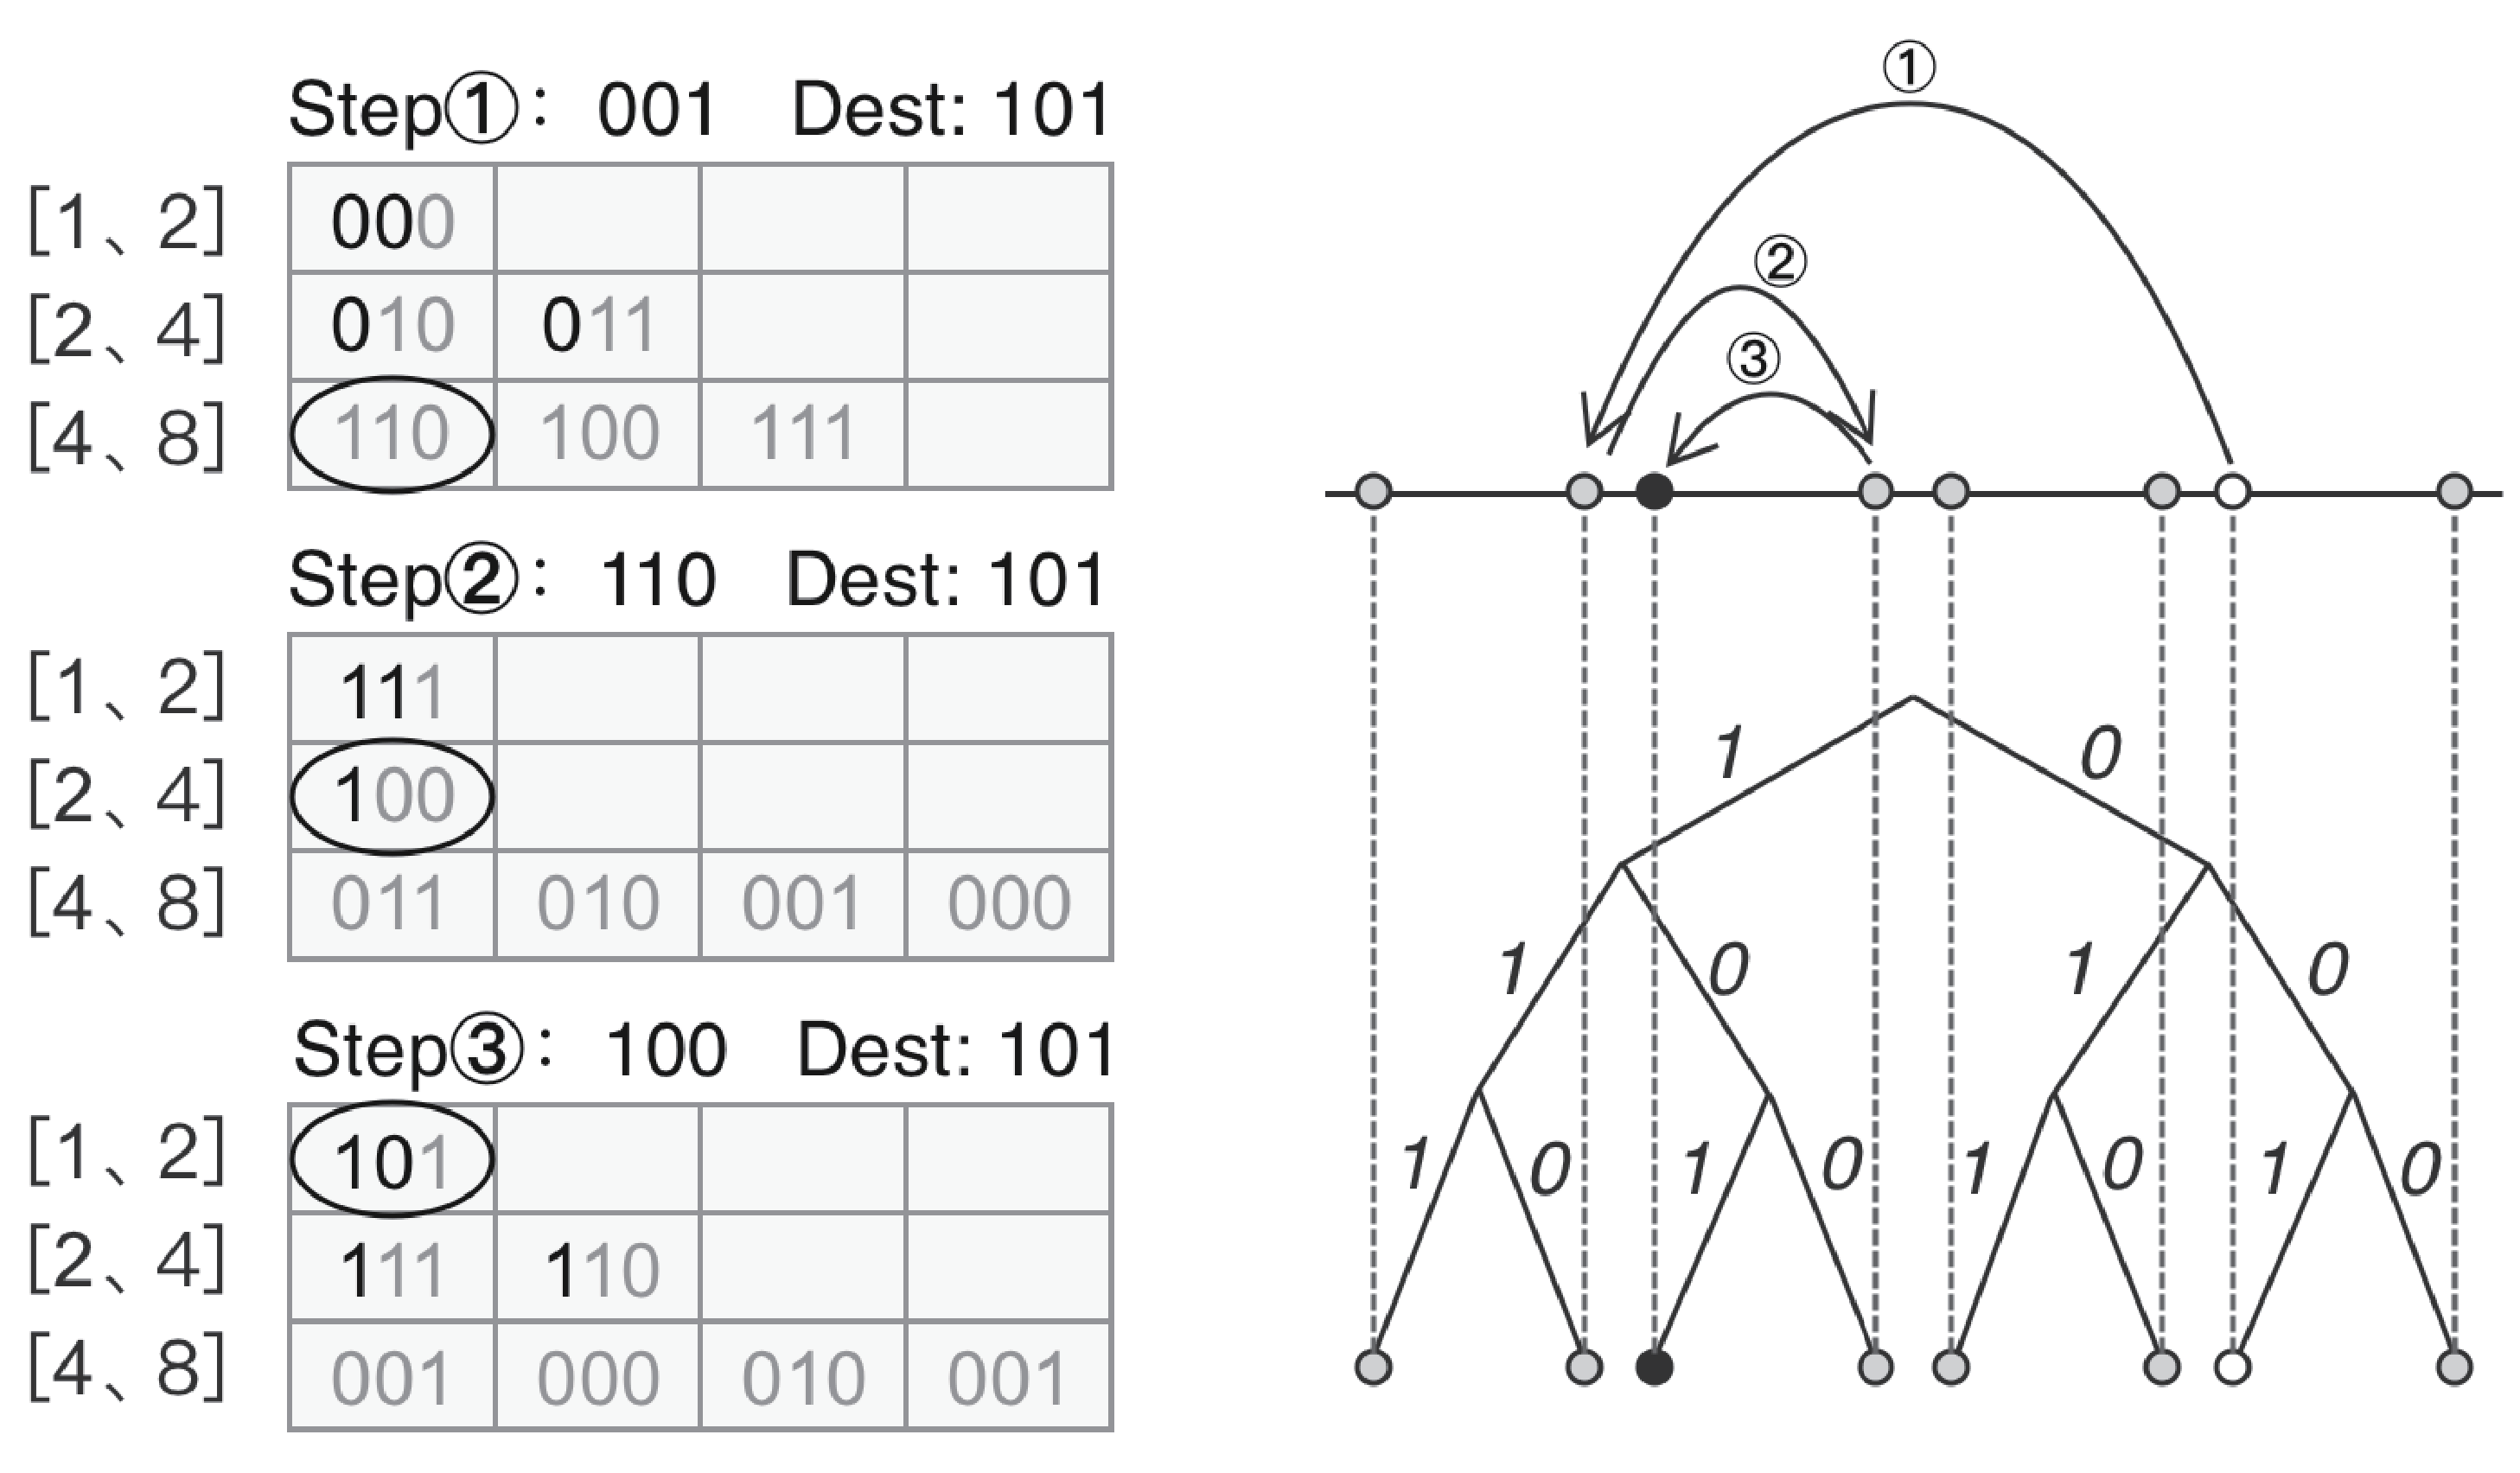
\includegraphics[width=320pt]{fig2}}
\\\\ \centerline{{Рисунок 2.2 Поиск в DHT Kademlia}}
\vspace{-0.5em}
\\
Так же, для увеличения безопасности сети, PPIO применяет расширение Kademlia-S/Kademlia \cite{article23}. В основном, данные изменения вызваны узлами, использующими параллельный поиск над непересекающимися путями.  Сеть может противостоять атакам даже при большом количестве скомпромитированных узлов.
\vspace{-0.5em}
\\ \\С приведенной выше реализацией DHT, такие структурированные данные как индекс файлов, статистики сетевых узлов и другие метаданные могут быть безопасно сохранены и быстро обнаруживаемы в  распределенной сети PPIO. Тем не менее, транспортировка данных в сети хранения происходит по другому, это бкдет освещено далее.
  \vspace{-0.5em}
\subsubsection{Одноранговые самоорганизующиеся оверлейные сети (P2P Self-organizing Overlay networks)}  %——2.2.3
         \vspace{-0.5em}
Современные промышленные сервисы хранения, такие как Amazon S3, Dropbox, Google Drive, iCloud и т.п., хранят пользовательские данные в больших дата-центрах. Из за дорогивизны, каждый такой сервис может разместить лишь ограниченное количество дата-центров по миру. На рисунке 2.3 показано распределение дата-центров Amazon AWS. В связи со специфичной природой интернета, довольно трудно гарантировать высокую скорость передачи данных в каждой точке земного шара, полагаясь на несколько дата-центров. Пользователяв одного региона приходится конкурировать за ширину канала связи к дата-центру. При возростании количества пользователей будет деградировать скорость транспортировки и удовлетворенность этих самых пользователей.
\vspace{-0.5em}
 \\ \\ \centerline{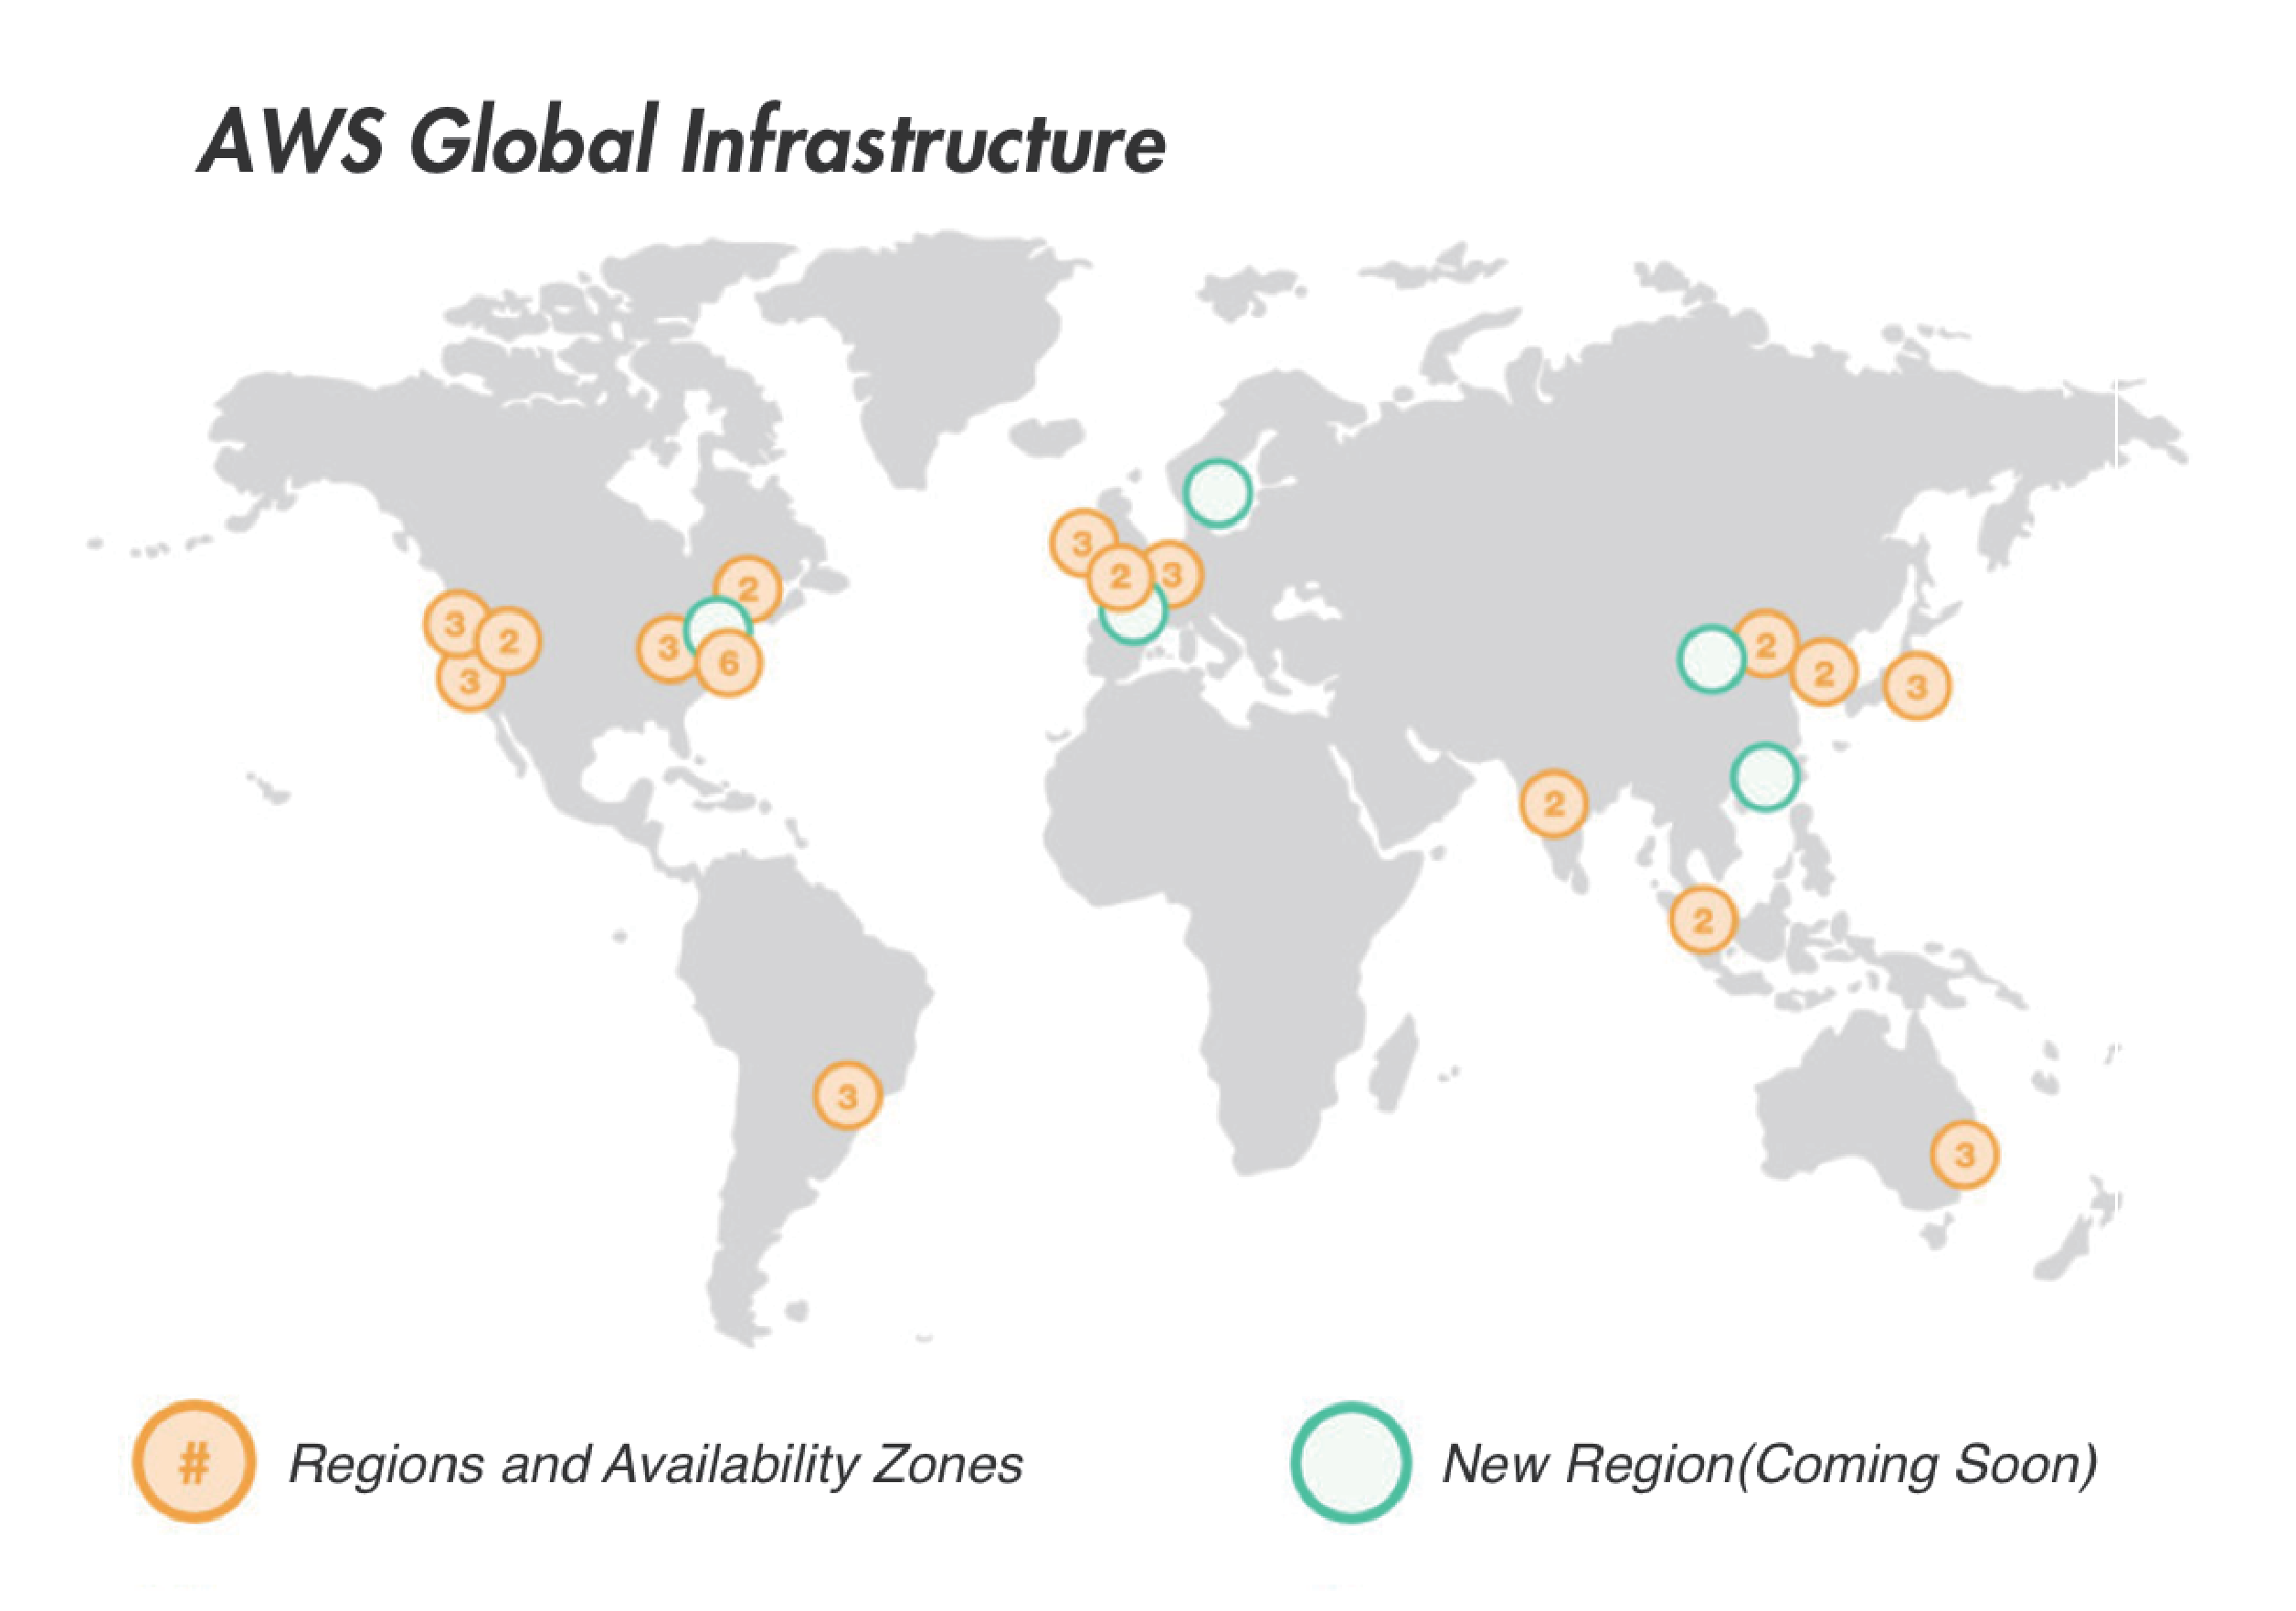
\includegraphics[width=340pt]{fig3}}
\\ \centerline{{Рисунок 2.3 Глобальная инфраструктура AWS}}
\\ \\ Распределенное хранилище PPIO является само организующейся, бесструктурной оверлейной сетью, со стимуляцией взаимодействия между локальными пирами. Для хранения данных с большой вероятностью будут выбраны майнеры, расположенные рядом. Аналогично, распространение и получение данных в основном обрабатывается рядом стоящими пирами. В результате, транспортировка данных может осуществляться с намного более высокой скоростью за счет полной утилизации локальных каналов связи.
\vspace{-0.5em}
\\ \\Чем больше узлов присоединяется к сети хранения PPIO, тем легче узлам становится отыскивать ближайших пиров с быстрыми соединениями, как для сохранения так и для получения данных. Ширина канала связи сервера более не является узким местом и пользователи получают лучшю скорость и удовлетворенность.
\vspace{-0.5em}
\\ \\{\bf Формирование само-организующейся одноранговой сети (Establishing a Self-Organizing P2P Network)}
\vspace{-0.5em}
\\ \\Каждый узел в сети PPIO обслуживает список соседних пиров с которыми он соединен. Список подвергается постоянному обновлению выбрасыванием отсоединившихся узлов и добавлением вновь присоединившихся соседей. В результате, список должен в основном содержать активных и быстрых соседей. В случае если все узлы следуют описанному выше сценарию, формируется и поддерживается само-организующаяся одноранговая оверлейная сеть.
\vspace{-0.8em}
\\

\hangafter 1
\hangindent 1.5em
\noindent   
•\quad Из пиров, с которыми имелось соединение в прошлом, формируется начальное множество соседей-кандидатов. Вновь присоединенные узлы начинают с пустым списком.
\vspace{-0.8em}
\\

\hangafter 1
\hangindent 1.5em
\noindent   
•\quad Из DHT Kademlia извлекаются новые соседи-кандидаты. Как упоминалось ранее, нет гарантии что эти пиры расположены близко в географическом плане или обладают быстрым каналом связи к узлу.
\vspace{-0.8em}
\\

\hangafter 1
\hangindent 1.5em
\noindent   
•\quad Предпринимается попытка установить соединение с кандидатами из упомянутых выше двух множеств, при этом число соединений не должно превзойти установленный лимит. Каждый соединенный узел считается соседом.
\vspace{-0.8em}
\\

\hangafter 1
\hangindent 1.5em
\noindent   
•\quad Периодически, отсмотром соседей соседей, получаются новые кандидаты.
\vspace{-0.8em}
\\

\hangafter 1
\hangindent 1.5em
\noindent   
•\quad Для каждого нового кандидата периодически замеряется и вычисляется скорость передачи, по принципу round-robin, кандидаты ранжируются по вычисленным значениям.
\vspace{-0.8em}
\\

\hangafter 1
\hangindent 1.5em
\noindent   
•\quad Более не доступные соседи, а так же соседи с малой скоростью соединения, исключаются.
\vspace{-0.8em}
\\

\hangafter 1
\hangindent 1.5em
\noindent   
•\quad Для замены исключенных соседей, из головы отранжированного перечня, выбираются новые кандидаты.
\vspace{-0.8em}
\\

\hangafter 1
\hangindent 1.5em
\noindent   
•\quad Весь процесс повторяется.
\vspace{-0.6em}
\\ 

\noindent  
Для выполнения изложенного выше процесса, каждый узел должен поддерживать в реальном времени два списка, список текущих соседей и список соседей-кандидатов. Так же, каждый узел поддерживает список бывших соседей. Все это является существенным для процедуры поиска узла в оверлейной сети.
\vspace{-0.5em}
\\ \\{\bf Приоритезация майнеров-хранителей с малой сетевой дистанцией (Preferred storage miners with a closer network distance)}
\vspace{-0.5em}
\\ \\Когда пользователь выгружает данные в сеть хранения PPIO, приоритет в выборе майнеров-хранителей для размещения данных отдается соседям с меньшей сетевой дистанцией. Для достижения более высокой скорости сохранения и получения данных, большой процент копий этих данных сохраняется на соседних майнерах с более быстрым соединением с пользователем. Когда достаточное количество узлов майнеров подключится к сети в различных регионах мира, высокая скорость скорость передачи данных может быть достигнута в рамках всей планеты.
\vspace{-0.5em}
\\ \\{\bf Пользователи, часто меняющие регион пребывания}
\vspace{-0.5em}
\\ \\В случае если узел пользователя постоянно путешествует между двумя различными регионами, архитектура PPIO может предложить замечательное решение для удобства пользователя в обоих местах. При нахождении пользователя в локации $A$, он находит соседей в этой самой локации $A$. Аналогично, при находжении пользователя в локации $B$,он находит соседей в локации $B$. В результате, его список соседей и исторический список содержит пиров из обоих локаций. Если пользователь остается в локации $A$ на длительный период, его список соседей будет содержать больше пиров локации $A$, и наоборот. Если пользователь постоянно перемещается туда и обратно, список будет содержать примерно одинаковое число пиров как из $A$ так и из $B$. В этом случае, когда узел пользователя выгружает данные, соседние майнеры из обоих локаций будут сохранять их копии, таким образом, быстро получить данные можно будет в обоих местах.
\vspace{-0.5em}
\\ \\{\bf Если пользователь окончательно перемещается в другой регион}
\vspace{-0.5em}
\\ \\В случае если узел пользователя перемещается в другой регион на постоянной основе, для облегчения перепланировки PPIO предлагает возможность сброса. При активации сброса, список соседей перестраивается с нуля. Для пользовательских данных в сети создаются новые копии, и эти копии сохраняются с приоритезацией новых соседей. В этом случае, для ранее сохраненных данных может быть обеспечено быстрое получение так же, как и для вновь сохраняемых в сети данных .
\vspace{-0.5em}


\subsubsection{Оптимизация доставки популярного контента}  %——2.2.4
В сети распространения данных, малое количество популярного контента может занять большую часть пропускной способности сети и ресурсов хранилищ. В то же время, скорость скачивания популярного контента может иметь существенное значение на пользовательские впечатления в целом. Таким образом, оптимизация доставки популярного контента является ключевым моментом в сети. PPIO предоставляетдва оптимизированных метода планирования доставки популярного контента, один из них, это "активнй выбор майнера" (Storage miners active selection), второй форсируется планировщиком (индексным узлом) ???. Оба метода спроектированы для совместного функционирования и увеличения эффективности распространения популярного контента и поддержания здоровой экосистемы сети хранения.
\vspace{-0.5em}
\\ \\{\bf Активный выбор майнера (Storage Miner active selection)}
\vspace{-0.5em}
\\ \\Как описывалось в секции 2.2.3, между узлами-участниками формируется само-организующаяся оверлейная сеть. Когда пользовательский узел запрашивает какую то часть данных, он в первую очередь отсматривает имеющиеся ресурсы на индексном узле, индексный узел возвращает информацию о узлах майнерах, хранящих желательный контент. В то же самое время, для поиска желательного контента, пользовательский узел широковещательно опрашивает своих соседей. По факту получения они будут пересылать запрос далее своим соседям. Для предоствращения излишней нагрузки на сеть, количество пересылок ограничено. Но, так же, количество пересылок адаптируется по количеству узлов, которых запрос достиг. Дальнейшие пересылки разрешены до тех пор, пока не достигнуто достаточное количество узлов.
\vspace{-0.5em}
\\ \\Когда узел майнера получает такой пересылаемый запрос, и если он обладает запрошенным ресурсом, он оповещает пользователя и, по факту, существует большая вероятность, что пользователь будет загружать данные именно с этого майнера, так как узел майнера расположен на пути пересылки среди соседей пользователя, и, соответственно, близок к нему. В PPIO майнер мотивирован предоставлять услугу скачивания так как получает за нее вознаграждение.
\vspace{-0.5em}
\\ \\В описанном выше процессе майнер может отслеживать запросы расположенных рядом пользователей и идентифицировать популярный контент. Обладание популярным контентом увеличивает шанс того что он будет скачан и оплачен, майнер будет заранее слать запросы планировщику на сохранение ресурса популярного контента. Если множество майнеров будет следовать этой стратегии, популярные данные быстро распространятся, и это значительно увеличит скорость скачивания для пользователей. Когда майнер обнаружит что хранимый им контент больше не в тренде, он может запросить его удаление из своего хранилища. После этого хранилище становится доступным для сохранения других ресурсов.
\vspace{-0.5em}
\\ \\Данный метод работает при наличии соответствующей необходимости и поощряет майнеров на проактивное обслуживание популярного контента. Так же, он адаптирован для популяризации данных в разных регионах. Оверлейная сеть PPIO строится в виде кластеров расположенных рядом пиров, и если какая то часть данных популярна в заданном регионе, то их широкое распространение будут производить только майнеры из этого же региона. Майнеры из других частей сети не затрагиваются. Это обеспечивает эффективность сети хранения в целом.
\vspace{-0.5em}
\\ \\Алгоритм идентификации популярного контента может быть изменен для каждого майнера. Различные майнеры в разных регионах могут модифицировать алгоритм по разному, для максимизации вознаграждения.
\vspace{-0.5em}
\\ \\{\bf Форсирование индексером}
\vspace{-0.5em}
\\ \\Для узлов майнеров, хранящих большое количество популярного контента, желательно получать больше запросов на скачивание и удовлетворять эти запросычтобы получать большее вознаграждение. Однако, чрезмерное конкуррентное скачивание будет переполять пропускную способность этих майнеров и приводить к уменьшению скорости скачивания для каждого пользователя. В то же самое время, не вполне честно, что майнеры, хранящие менее популярный контент, получают много меньшее вознаграждение чем остальные.
\vspace{-0.5em}
\\ \\Для предотвращения этих проблем сетевой планировщик (индексер) предоставляет выделенную услугу планирования, основанную на популярности контента. Майнеры, запрашивающие на хранение наиболее популярный контент, должны заплатить планировщику (индексеру) перед тем как получат ресурсы. Узлы майнеров с широким каналом связи и большим объемом хранилища, имеют достаточно мотивации для такой оплаты, но не желают получать слишком много такого контента. Иначе, они не смогут обслуживать избыточные данные предоставлением услуги скачивания, умещающуюся в ширину канала.
\vspace{-0.7em}
 \\ \\\\
\centerline{\includegraphics[width=300pt]{fig4}}
\\\\\centerline{{Рисунок 2.4 Доставка популярного контента}}
\vspace{-1.5em}
\\ \\ Как показано на Рис 2.4, множество майнеров хранят копии одних и тех же данных, они должны конкурировать за предоставление пользователям услуги скачивания. Пользователи всегда выбирают тех, кто предоставляет более высокую скорость скачивания. Если майнер не обладает достаточной шириной канала, пользователи переключаться на других. Количество отгруженных пользователям данных уменьшится, что приведет к уменьшению полученного вознаграждения. С другой стороны, майнеры с малой шириной канала не будут замотивированы на хранение популярного контента. В результате, популярный контент в основном сосредоточится у майнеров с широким каналом, что приведет к увеличению скорости и удовлетворенности пользователя при скачивании такого контента.
\vspace{-0.5em}
\subsubsection{Планирование, дружественное к интернет-провайдеру (ISP Friendly Scheduling)}  %——2.2.5 \%     \cite{article33}
В большинстве одноранговых сетей, узел может обмениваться данными с любым другим пиром, не взирая на его местоположение. As a result, a single data transfer can potentially create traffic anywhere in the world and consumes bandwidth between different Internet Service Providers (ISP), or even between different countries. In 2007, a research institute iPoque carried out an analysis on nearly 3TB of anonymous data sampled from more than a million internet users in Eastern Europe, Southern Europe, Australia, and the Middle East \cite{article26}. Their studies show that P2P file sharing takes up a significant part of the network bandwidth consumption, accounting for about 49\% in the Middle East, and 84\% in Eastern Europe. From a global perspective, 95\% of the bandwidth at prime time is involved in some forms of P2P data transmission. In recent years, the percentage of P2P traffic has dropped due to a shift in the use pattern of Internet applications. However, with the recent development of blockchain technology and decentralized applications, P2P network traffic is expected to start increasing again. P2P traffic consumes an extraordinary amount of network bandwidth, including international bandwidth. It puts a lot of burden on our internet infrastructure, and significantly increase the cost for ISPs to operate.
\vspace{-0.5em}
 \\ \\As described in section 2.2.3, PPIO’s self-organizing overlay network encourages data transfer among neighboring nodes, a large percentage of its traffic is contained within the local network, and the operation cost incurred upon ISPs is significantly reduced. However, the  topology of PPIO’s overlay network may not match the ISP topology exactly. Further optimization to reduce unnecessary traffic between ISPs is needed to improve further PPIO’s ability to scale globally.
 \vspace{-0.5em}
 \\ \\If the nodes participating in a data transmission happen to be in the close vicinity of each other, it is likely that the traffic will be contained within their area network. As a result, the bandwidth cost will be significantly reduced. This is the principle behind P4P, to fully utilize local network bandwidth in a P2P network.  
 \vspace{-0.5em}
  \\ \\ P4P, or Proactive network Provider Participation for P2P \cite{article17}, is a method for ISPs and P2P software to optimize connections []. It enables peer selection based on the topology of the physical network, to reduce traffic on the backbone network, lower the operation cost of network providers, and improve data transfer efficiency. 
  \vspace{-0.5em}
  \\ \\The implementation of P4P in traditional P2P networks relies on central servers. As PPIO is a completely decentralized network, a decentralized P4P solution is required.
  \vspace{-0.5em}
    \\ \\PPIO provides an iP4P interface that allows ISPs to set up and configure P4P in their network and allows applications to query the information. iP4P is designed to be similar to the iTracker interface \cite{article17} in centralized P2P networks, to make it easier to adapt.
    \vspace{-0.8em}
%•\quad \hl 
\\

\hangafter 1
\hangindent 1.5em
\noindent   
•\quad{\bf ip-list}: allows ISPs to provide the list of IPs in their network, it allows nodes in PPIO’s network to be associated with their ISP.
\vspace{-0.8em}                                                      %           {\color{red} $ip-list$}---------给文字加颜色                                                                 %   \hl{-}--------给文字加背景颜色,结合宏
\\

\hangafter 1
\hangindent 1.5em
\noindent   
•\quad{\bf policy}: allows ISPs to configure the policy for applications to access P4P information.
\vspace{-0.8em}
\\

\hangafter 1
\hangindent 1.5em
\noindent   
•\quad{\bf p4p-distance}: allows applications to query P4P cost and distance between network nodes.
\vspace{-0.8em}
\\

\hangafter 1
\hangindent 1.5em
\noindent   
•\quad{\bf capability}: allows applications to query of network resources and capacity of the ISP network.
\vspace{-0.8em}
\\

\hangafter 1
\hangindent 1.5em
\noindent   
•\quad{\bf firendly-isp-list}: allows applications to query information of friendly ISP, including p4p-distance across different ISPs.
\vspace{-0.6em}
\\

\noindent 
At the same time, PPIO introduces a global IP database that is maintained by the community. Information in the database can be used to calculate the p4p distance between two nodes in the network when at least one of them is not within a known ISP network from the iP4P Interface. The database is synced to scheduler(Indexer) nodes and Verifier nodes in the P2P network. Every node in the network can query its information from the database. The following shows part of the information stored for each node.\\\\
\begin{tabular}{r|l}
&message P4PPeerInfo   \{ \\
	&\qquad uint32 countryId = 1;   //  Country ID \\
	&\qquad uint32 ispId = 2;       //  ISP ID  \\ 
	&\qquad uint32 stateId = 3;     // State or  Province ID \\
	&\qquad uint32 cityId = 4;      // City ID  \\ 
	&\}   \\ 
	
\end{tabular} \\
  \vspace{-0.5em}
\\\\
\noindent 
When selecting data connections from a given node, the indexing and scheduling node (Indexer) in PPIO’s network checks whether the node can be queried from the iP4P interface:  
\vspace{-0.8em}
\\  

\hangafter 1
\hangindent 1.5em
\noindent   
•\quad If so, a peer lookup in the node’s ISP network will be conducted first, followed by a lookup in the friendly ISPs, and finally among all other peers. The final peer decision will still be decided based on connection speed as described in 2.2.3. In this way, peers with shorter p4p distances to the node are more likely to be selected to upload or download its data. At the same time, nodes in slower ISPs can still connect to faster outside peers. As a result, unnecessary traffic between different network providers is significantly reduced, and user experience across the entire network is maintained at a high-level.
\vspace{-0.8em}
\\

\hangafter 1
\hangindent 1.5em
\noindent   
•\quad  If not,the p4p distance calculated from the global IP database is used in the pre-selection of peers. Similarly, the final selection will still be based connection speed.
\vspace{-0.8em}

 
         \subsubsection{PCDN}  %——2.2.6
PCDN stands for CDN acceleration with P2P, and it utilizes the abundant bandwidth and storage resources of miners in the P2P network to achieve faster data distribution. PPIO is designed to support PCDN and provide an easy-to-use interface to DApps to accelerate their content delivery. 
\vspace{-0.5em}
\\ \\It is published on the source node first to start distributing a piece of content. As long as the source node is online, the user can download them from it. However, as the number of users downloading from the same source node increases, its available bandwidth gets quickly exhausted, and the downloads will slow down. With PCDN, when other miner nodes start to store and provide download services for the same piece of content, users will be able to download from multiple peers in the network and enjoy much better user experience.\\
\centerline{\includegraphics[width=300pt]{fig5}}
\vspace{-0.5em}
 \\ \centerline{{Figure 2.5 PCDN Data Flow}}
\vspace{-0.5em}
 \\ There are two ways for applications to implement PCDN in PPIO.
\vspace{-0.7em}
\\

\hangafter 1
\hangindent 1.7em
\noindent   
1.\quad Take advantage of content scheduling described in 2.2.4.  As PPIO embeds optimized scheduling of popular contents in its overlay network,  the miners will proactively download and store these data, and provide download services. As a result, data gets copied and distributed across the network where the data is deemed popular. It improves download experience as the number of copies increase. 
\vspace{-0.7em}
\\

\hangafter 1
\hangindent 1.7em
\noindent   
2.\quad Enable and configure PCDN directly. PPIO provides a set of APIs to allow DApps to set up PCDN for their content. The applications can specify the number of copies to be maintained in specific parts of the network, or specific geographic location regarding the country, ISP, state and city, as defined in the P4P database. PPIO will find the miner nodes in the specified area to store the copies and provide download services. As the scheduling is specified by the application, it needs to compensate the miners’ cost in storage spacetime, scheduling and conducting storage proofs. Figure 2.5 shows the PCDN-driven data flow in the network in this case.
\vspace{-1em}


         \subsection{Proofs}%——2.3
PPIO employs 4 different storage proofs, namely Proof of Replication (PoRep), Proof of Download (PoD), Proof of Spacetime (PoSt) and Light Proof of Capacity (LPoC). These proofs guarantee that the storage provider (miner) correctly replicates the data and consistently stores the data within the agreed period. They also ensure that user can successfully download the data any time during the agreed term. These proofs maintain the integrity and reliability of PPIO's storage system. They will be discussed in details in this section.
\vspace{-0.5em}
\\ \\Definition of terms in the section:
\vspace{-0.8em}
\\

\hangafter 1
\hangindent 1.5em
\noindent   
•\quad CRH: Collision-Resistant Hashing, a hash function h with which it is very tough to find two different inputs x, x', and generate the same output h(x) == h(x').
\vspace{-0.8em}
\\

\hangafter 1
\hangindent 1.5em
\noindent   
•\quad MerkleCRH: The root hash of a Merkle tree built from collision resistant hashing. Merkle tree can be used as an efficient way to validate if the content of a data block matches the original data.
\vspace{-0.8em}
\\

\hangafter 1
\hangindent 1.5em
\noindent   
•\quad Seal: An encryption method to ensure that each copy of the data has a unique and independent representation. The encryption process should take substantially longer time than decryption, to prevent Generation Attacks. AES-256 is a viable option for its implementation.
\vspace{-0.8em}
\\

\hangafter 1
\hangindent 1.5em
\noindent   
•\quad Cipher: A lightweight encryption method with symmetric keys, used in Proof-of-Download. XOR Cipher is a viable option for its implementation.  
\vspace{-0.5em}

               \subsubsection{Proof-of-Replication (PoRep)}  %——2.3.1
               
Proof of Replication (PoRep) provides a way to verify that Miner $L$ correctly replicates Data $D$ from User $U$ and stores it in its storage. The process also provides an indirect proof of the bandwidth available to $L$. The procedure of PoRep is described below.
\vspace{-0.8em}
\\ \\ 
\centerline{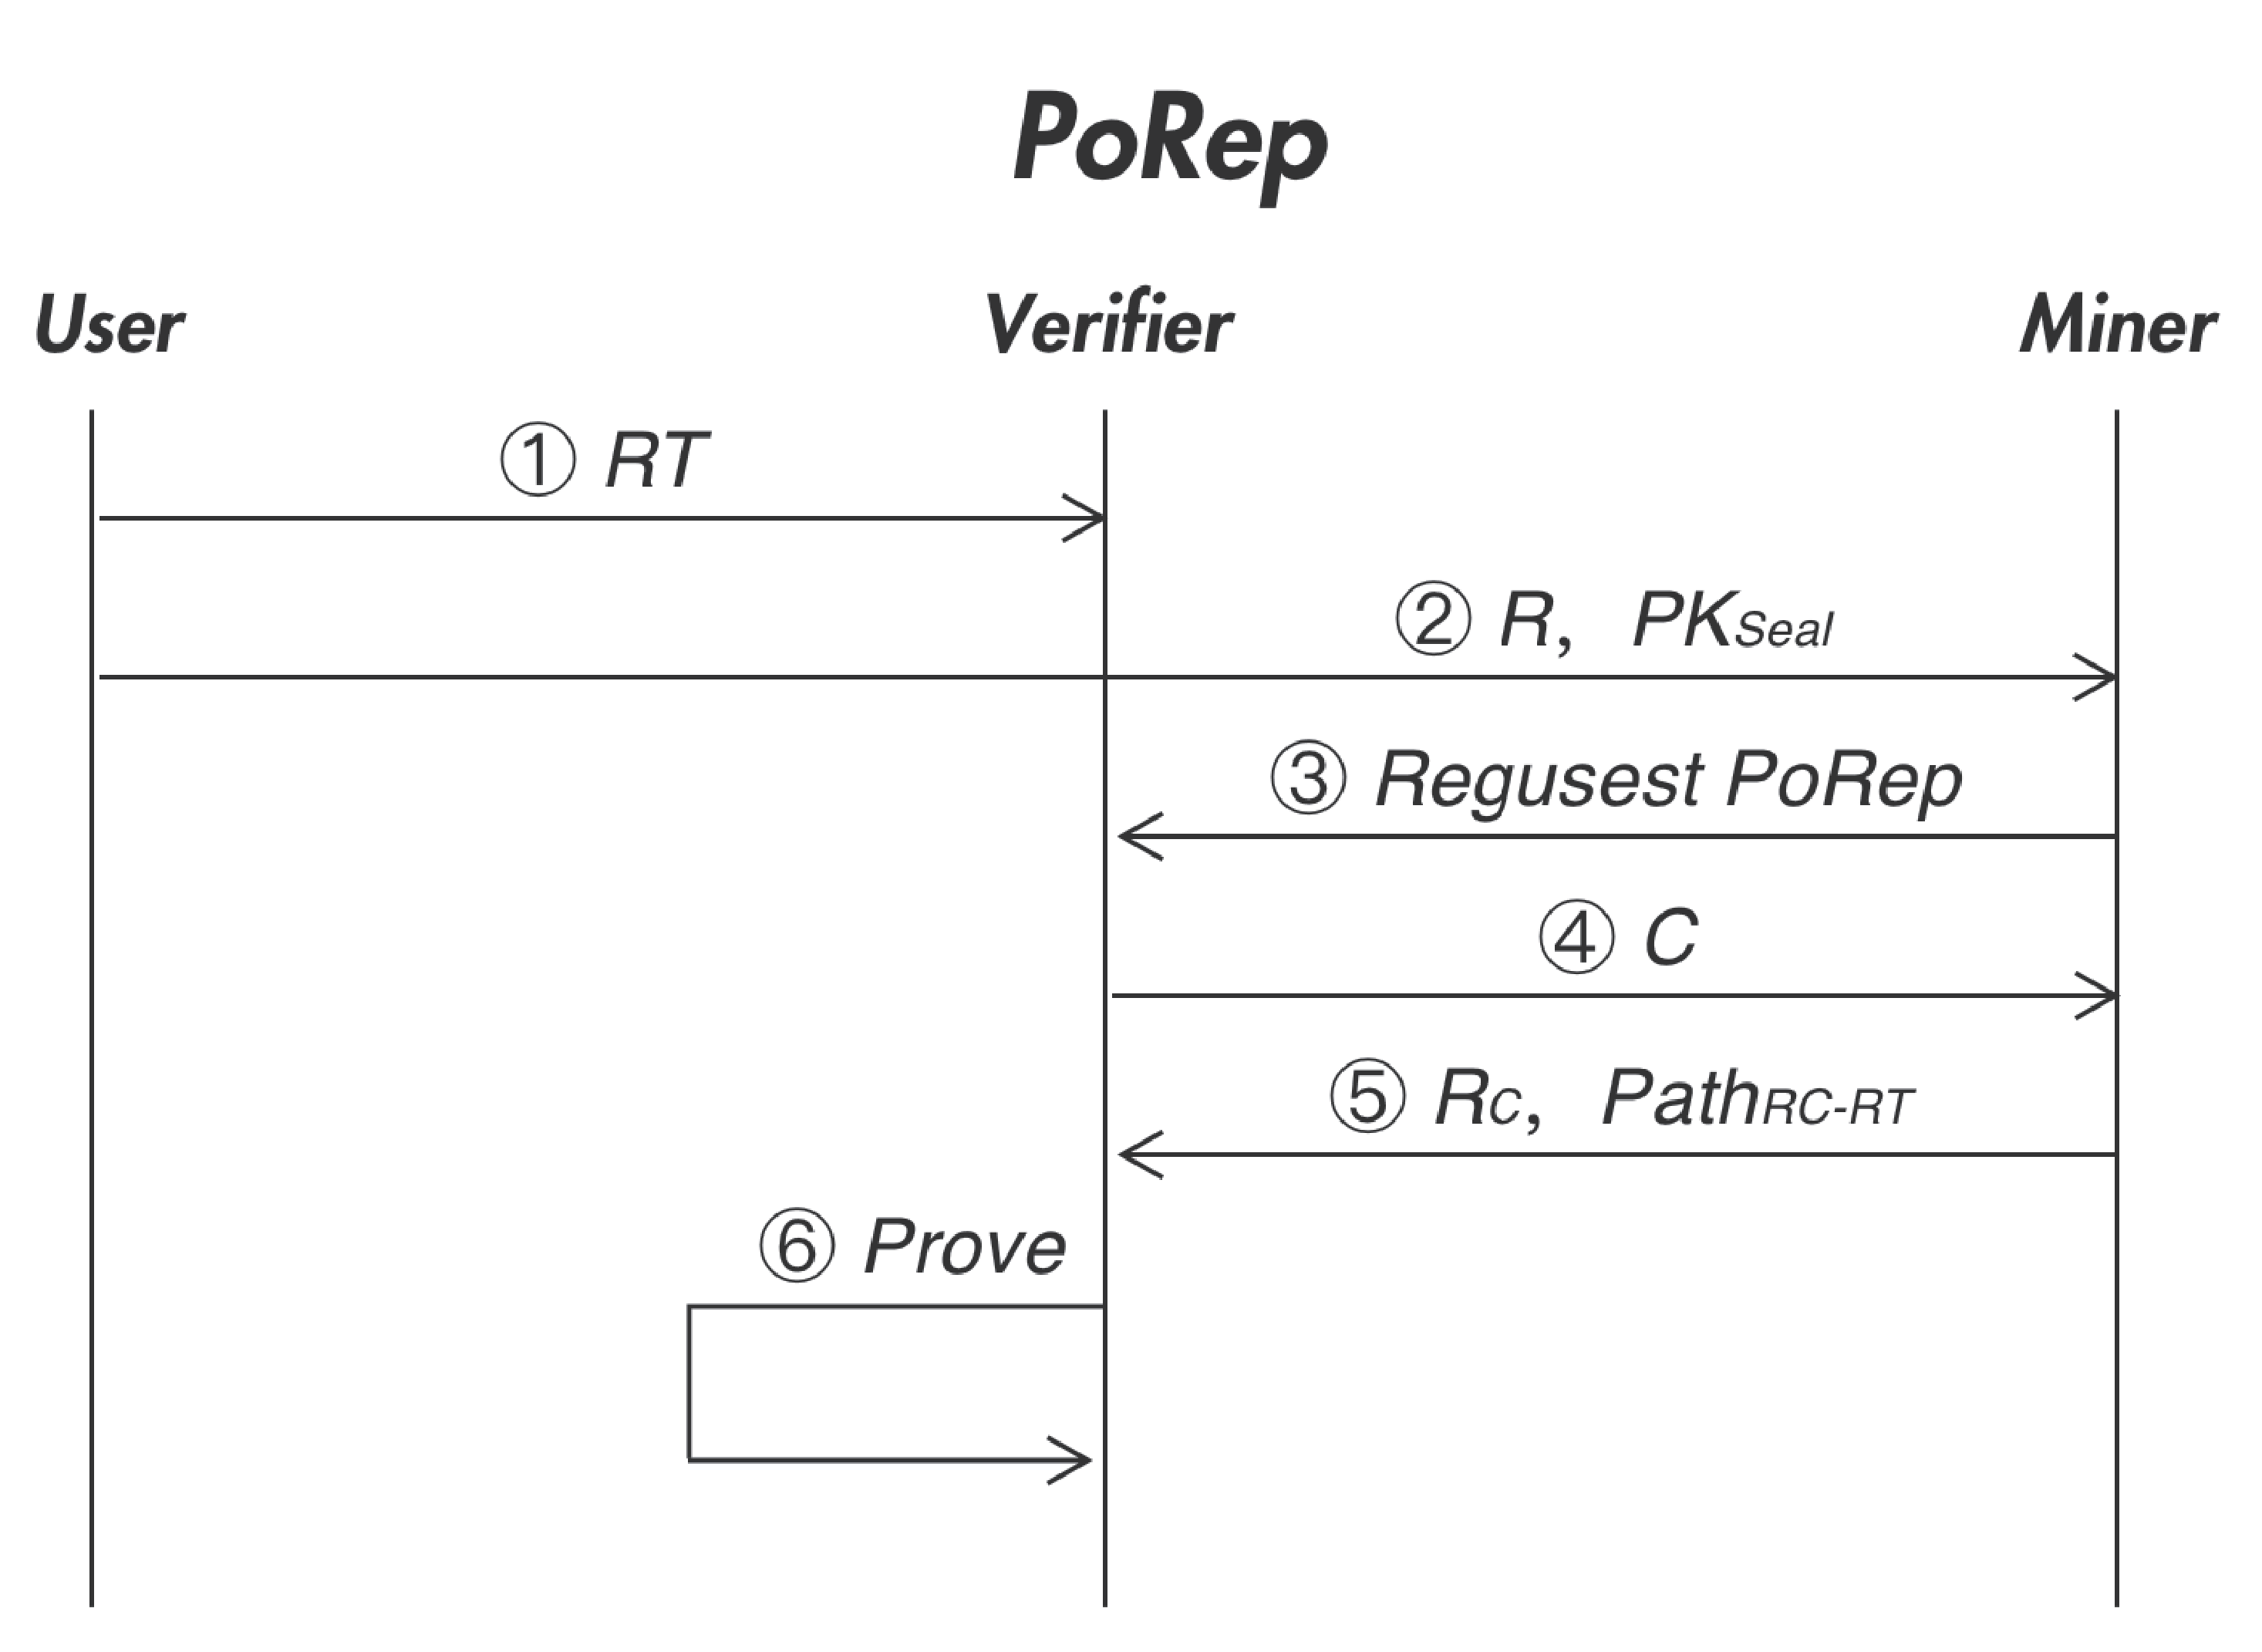
\includegraphics[width=320pt]{fig6}}
\\ \\\centerline{{Figure 2.6 Proof-of-Replication}}
\vspace{-1.5em}
\\

\hangafter 1
\hangindent 1.7em
\noindent   
1.\quad User $U$ generates a Seal key $PK_{Seal}$, applies it to encrypt Data $D$, and generates a unique copy $R=Seal(D, PK_{Seal})$. It also builds a Merkle Tree on top of $R$, calculates the root hash of the tree $RT=MerkleCRH(R)$, and sends $RT$ to Verifier $V$.
\vspace{-0.8em}
\\

\hangafter 1
\hangindent 1.5em
\noindent   
2.\quad $U$ transmits $R$ and $PK_{Seal}$ to miner $L$.
\vspace{-0.8em}
\\

\hangafter 1
\hangindent 1.7em
\noindent   
3.\quad $L$ requests PoRep challenge from $V$, $V$ accepts the request and sends a random challenge $c$ to $L$, i.e. it challenges the storage of the $c$th data block of $R$.
\vspace{-0.8em}
\\

\hangafter 1
\hangindent 1.7em
\noindent   
4.\quad $L$ retrieves $R_{c}$ which is the $c$th block of $R$, and calculates $Path_{RC-RT}$ which contains the hash values of all the Merkle tree nodes path from the $R_{c}$ to the root node. $L$ returns the following to $V$:
\\•   $R_{c}$\\ 
     •  $Path_{RC-RT}$
     \vspace{-0.5em}
\\

\hangafter 1
\hangindent 1.7em
\noindent   
5.\quad From received $R_{c}$ and $Path_{RC-RT}$, $V$ generates the Merkle tree root hash $RT'$, if $RT'$ matches the original root hash received from $U$, i.e. $RT' == RT$, the proof has succeeded, otherwise the proof has failed.  
\vspace{-0.5em}
\subsubsection{Proof-of-Download (PoD)}  %——2.3.2
Proof-of-Download (PoD) provides a way to verify that Data $D$ has been correctly downloaded from the Miner $L$ to User $U$. The procedure of PoD is described below.
\vspace{-0.5em}
\\ \\
\centerline{\includegraphics[width=300pt]{fig7}}
 \\ \centerline{{Figure 2.7 Proof of Download}}
 \vspace{-1.5em}
\\

\hangafter 1
\hangindent 1.7em
\noindent   
1.\quad For Data $D$ to be downloaded, User $U$ sends the root hash of its Merkle tree $DT_{U}=MerkleCRH(D)$ to Verifier $V$.
\vspace{-0.8em}
\\

\hangafter 1
\hangindent 1.7em
\noindent   
2.\quad The miner $L$ decrypts its stored copy $R$ and obtains data $D$. It then calculates the root hash of its Merkle tree $DT_{L}=MerkleCRH(D)$.
\vspace{-0.8em}
\\

\hangafter 1
\hangindent 1.7em
\noindent   
3.\quad $L$ creates a Cipher Key $PK_{Cipher}$, applies it to Data $D$, and generates a ciphered copy $R'=Cipher(D, PK_{Cipher})$. It then calculates the root hash $R'T=MerkleCRH(R')$, and sends the following to $V$:
\\•  $DT_{L}$ \\ 
   •  $PK_{Cipher}$ \\ 
   •  $R'T$ 
   \vspace{-0.5em}
\\

\hangafter 1
\hangindent 1.7em
\noindent   
4.\quad $V$ checks whether $DT_{U}$ is identical to $DT_{L}$. If not, the proof has failed.
\vspace{-0.8em}
\\

\hangafter 1
\hangindent 1.7em
\noindent   
5.\quad $V$ sends a random challenge $c$ to $L$, i.e. the storage challenge of the $c$th block of $D$ and $R'$.
\vspace{-0.8em}
\\

\hangafter 1
\hangindent 1.7em
\noindent   
6.\quad $L$ retrieves $D_{c}$ which is the $c$th block of $D$ and calculates $Path_{DC-DT}$ which contains the hash values of all the Merkle tree nodes path from the $D_{c}$ to the root node. $L$ also retrieves $R'_{c}$ which is the $c$th block of $R'$ and calculates $Path_{R'C-R'T}$ which contains the hase values of all the Merkle tree nodes path from the $R'_{c}$ to the root node. It then returns the following to $V$:
\\
    •  $D_{c}$\\
   •  $Path_{DC-DT}$\\
   •  $Path_{R'C-R'T}$
   \vspace{-0.5em}
\\

\hangafter 1
\hangindent 2.2em
\noindent   
7.\quad \, From received $D_{c}$ and $Path_{DC-DT}$, $V$ generates the Merkle tree root hash $DT'_{L}$, and verifies that $DT'_{L}$ matches the root hash $DT_{L}$ previously received from $L$, i.e. $DT'_{L} == DT_{L}$. If not, the proof has failed.
\vspace{-0.8em}
\\

\hangafter 1
\hangindent 2.2em
\noindent   
 8.\quad\;\,From received $D_{c}$ and $PK_{Cipher}$, $V$ generates ciphered data block $R'_{c}=Cipher(D_{c}, PK_{Cipher})$, and calculates the root hash $R'T'$ using $R'_{c}$ and received $Path_{R'C-R'T}$, and verifies that $R'T'$ matches the root hash previously received $R'T$ from $L$, i.e. $R'T' == R'T$. If not, the proof has failed.
\vspace{-0.8em}
\\

\hangafter 1
\hangindent 2.2em
\noindent   
   9.\quad  \,    $U$ downloads data $R'$ from $L$.
\vspace{-0.8em}
\\

\hangafter 1
\hangindent 1.5em
\noindent   
10.\quad $U$ requests proof of download from $V$.
\vspace{-0.8em}
\\

\hangafter 1
\hangindent 2.2em
\noindent   
11.\quad  $V$ sends a random challenge $c$ to $U$, i.e. the storage challenge of the $c$th block of $R'$.
\vspace{-0.8em}
\\

\hangafter 1
\hangindent 2.2em
\noindent   
12.\quad $U$ retrieves $R'{c}$ which is the ${c}$th block of content on $R'$, and calculates $Path{R'C-R'T}$, which contains the hash values of all the Merkle tree nodes path from the $R'_{c}$ to the root node, and sends following to $V$:
\\
    •  $R'_{c}$ \\
   •  $Path_{R'C-R'T}$
    \vspace{-0.5em}
\\

\hangafter 1
\hangindent 2.2em
\noindent   
13.\quad From received $R'_{c}$ and $Path_{R'C-R'T}$, $V$ generates the Merkle tree root hash $R'T"$, if $R'T"$ matches the root hash $R'T$ previously received from $L$, i.e. $R'T" == R'T$, the proof has succeeded, and $V$ sends the Cipher key $PK_{Cipher}$ to $U$, so that $U$ can decipher $R'$ to recover data $D$ successfully.
\vspace{-0.5em}

        \subsubsection{Proof-of-Spacetime (PoSt)}  %——2.3.3
Proof of Spacetime (PoSt) provides a way to verify that Miner $L$ has stored Data $D$ for a given period. The process also provides an indirect proof of the storage capacity of $L$. The procedure of PoSt is described below.
\vspace{-0.5em}
\\ \\
\centerline{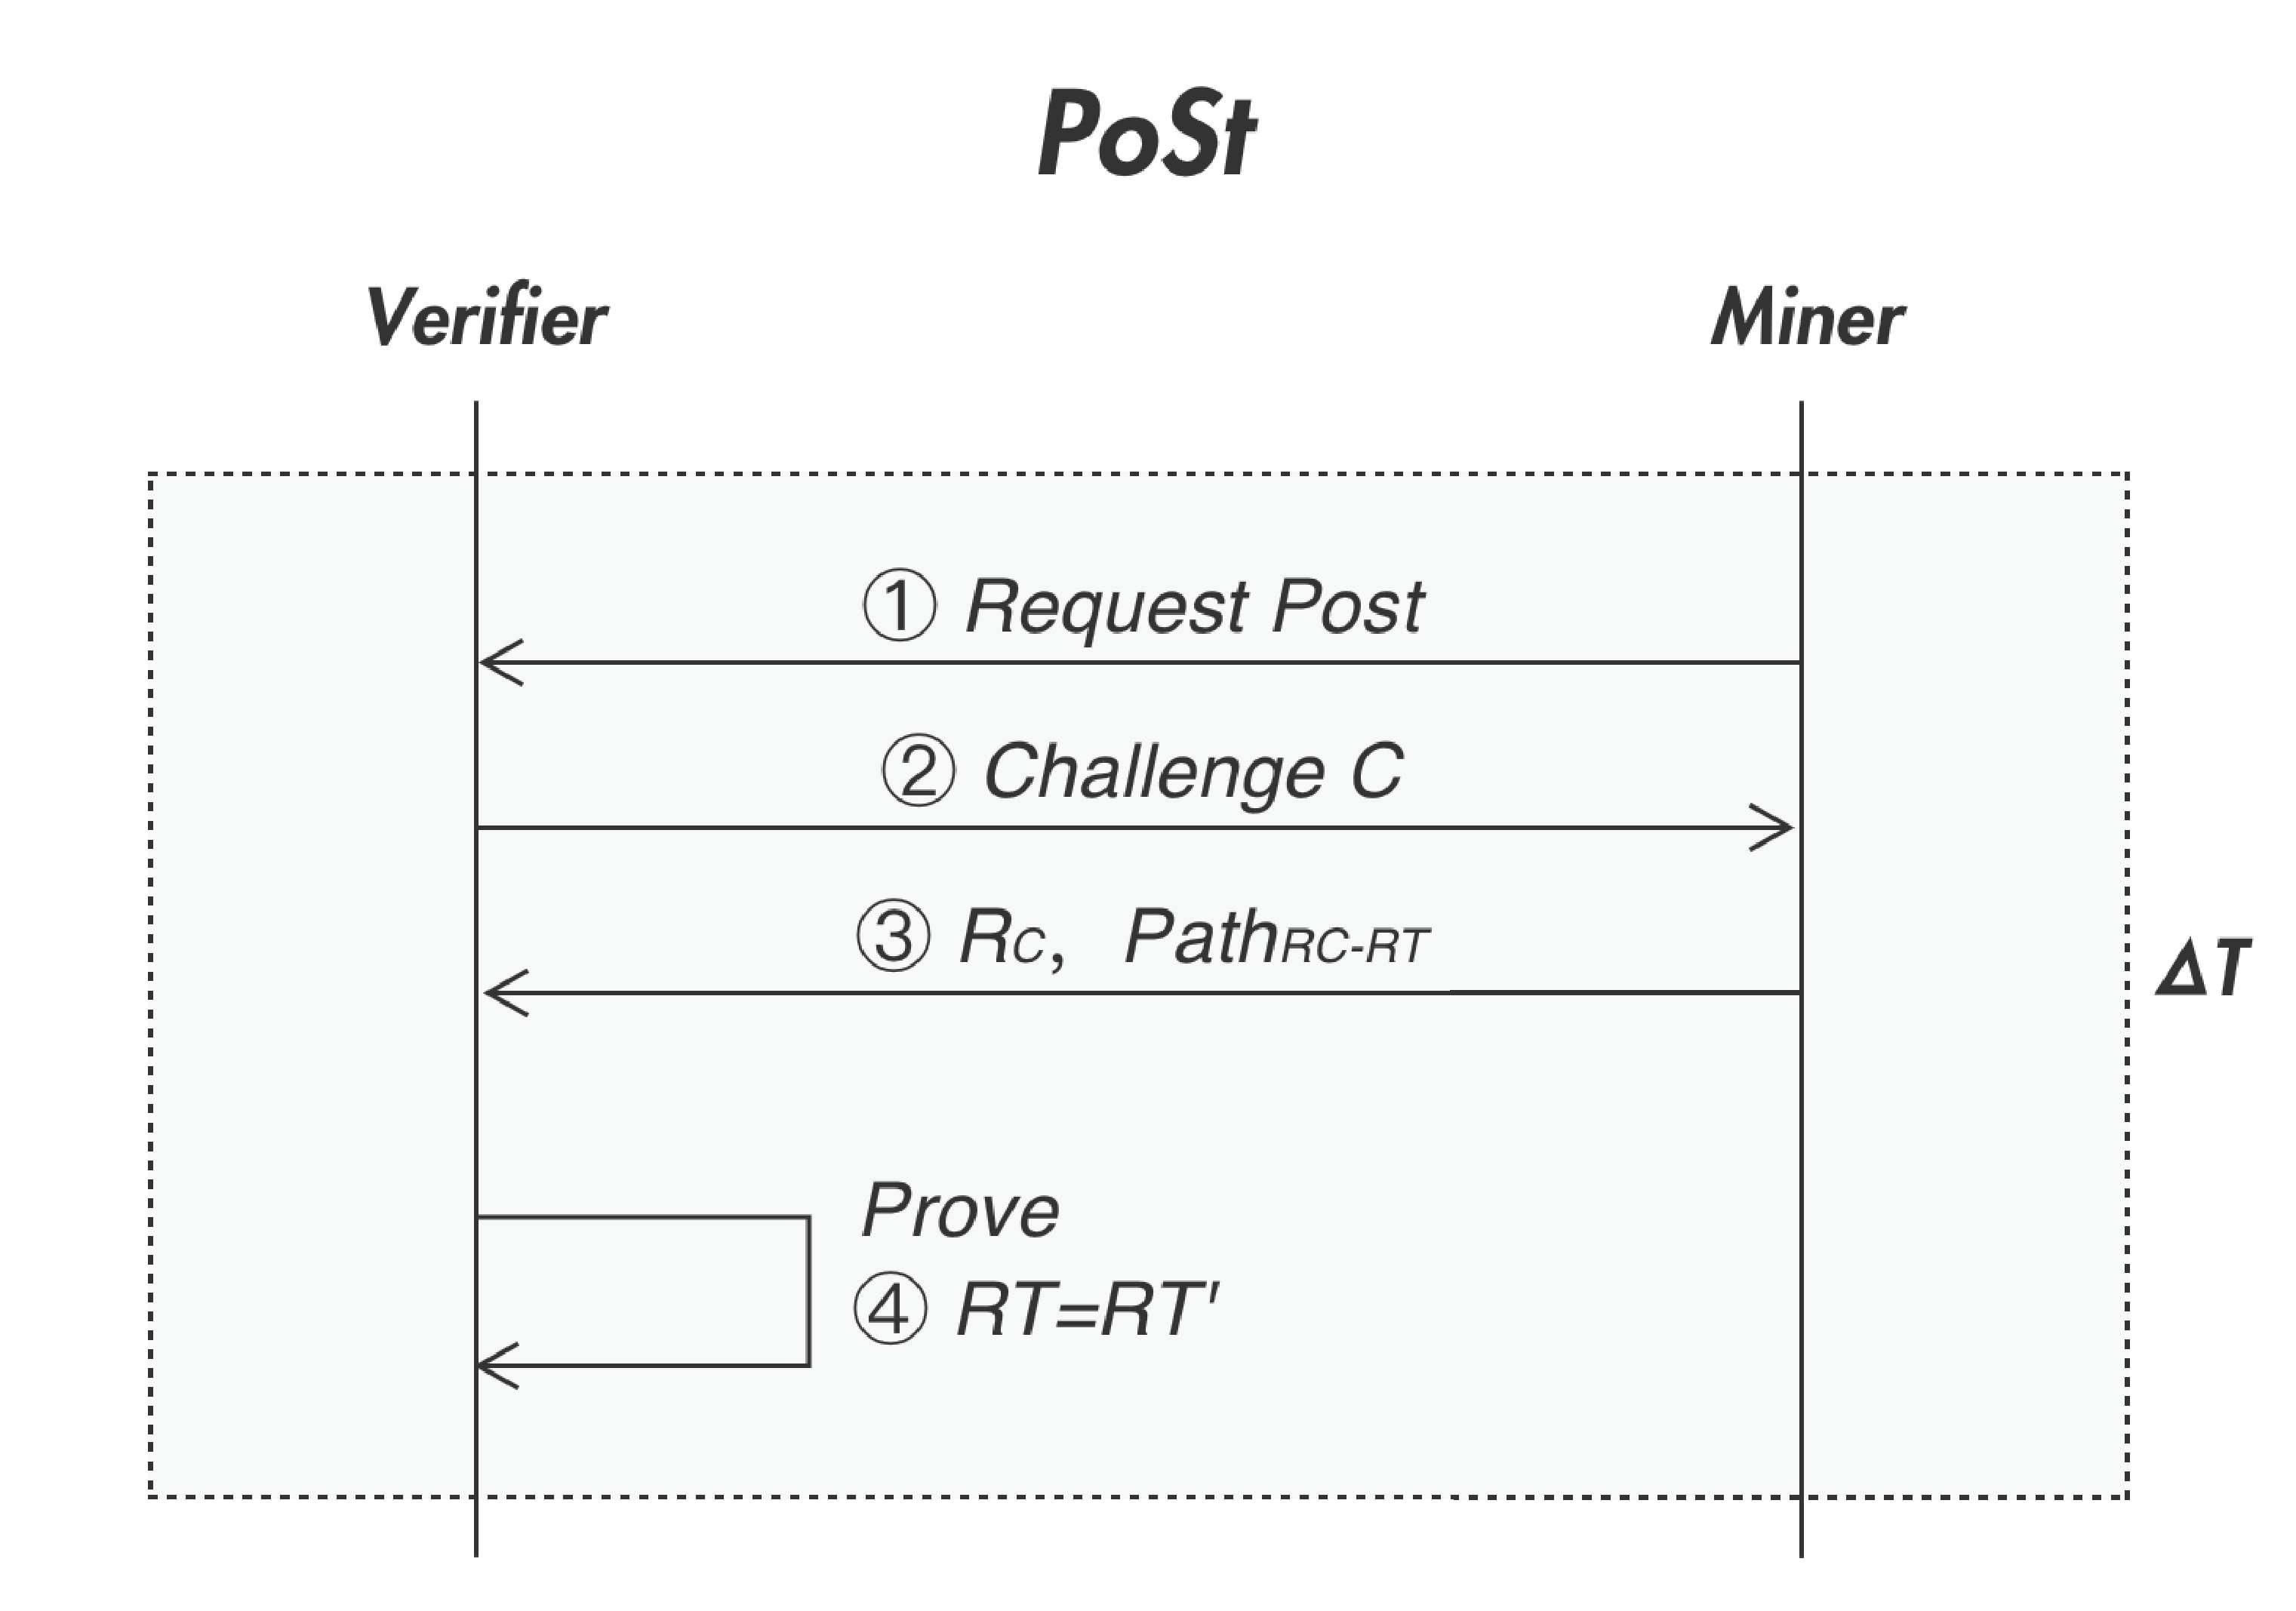
\includegraphics[width=380pt]{fig8}}
 \\\centerline{{Figure 2.8 Proof of Spacetime}}
 \vspace{-1.5em}
\\

\hangafter 1
\hangindent 1.7em
\noindent   
1.\quad As described in PoRep procedures, data $D$ is encrypted to obtain a unique copy $R$, $R$ is stored on $L$, its Merkle tree root hash is $RT=MerkleCRH(R)$.
\vspace{-0.8em}
\\

\hangafter 1
\hangindent 1.5em
\noindent   
2.\quad $V$ also stores $RT$.
\vspace{-0.8em}
\\

\hangafter 1
\hangindent 1.5em
\noindent   
3.\quad At a given time $T$, $L$ requests proof of storage challenge from $V$.
\vspace{-0.8em}
\\

\hangafter 1
\hangindent 1.5em
\noindent   
4.\quad $V$ sends a random challenge $c$ to $L$, i.e. the storage challenge on $c$th block of $R$.
\vspace{-0.8em}
\\

\hangafter 1
\hangindent 1.5em
\noindent   
5.\quad $L$ retrieves $R_{c}$ which is the $c$th block of $R$, and calculates $Path_{RC-RT}$ which contains the hash values of all the Merkle tree nodes path from the $R_{c}$ and the root node, and sends the following to $V$:
 \\   •  $R_{c}$\\ 
   •  $Path_{RC-RT}$
   \vspace{-0.5em}
\\

\hangafter 1
\hangindent 1.8em
\noindent   
6.\quad From received $R_{c}$ and $Path_{RC-RT}$, $V$ generates the Merkle tree root hash $RT'$, and verifies that $RT'$ matches the original root hash stored $RT$, i.e. $RT'==RT$. If not, the proof has failed.\\
\vspace{-0.8em}

\hangafter 1
\hangindent 1.5em
\noindent   
7.\quad  Repeat steps 3 to 6 at given time intervals.
\vspace{-0.8em}
\\

\hangafter 1
\hangindent 1.9em
\noindent   
8.\quad The series of repeated successful challenges and proofs between $L$ and $V$ generates the successful proof of spacetime.
\vspace{-0.5em}
        \subsubsection{Light-Proof-of-Capacity (LPoC)}  %——2.3.4
Light Proof of Capacity (LPoC) provides a way to verify the available storage capacity of miner $L$. The available capacity does not include the storage space already used for existing data. PPIO's lightweight proof reduces the number of resources wasted on conducting complicated proofs. The procedure of LPoC is broken into two phases, which are described below.
\vspace{-0.5em}
\\

\noindent   
 {\bf Initialization Phase }\\\\
\centerline{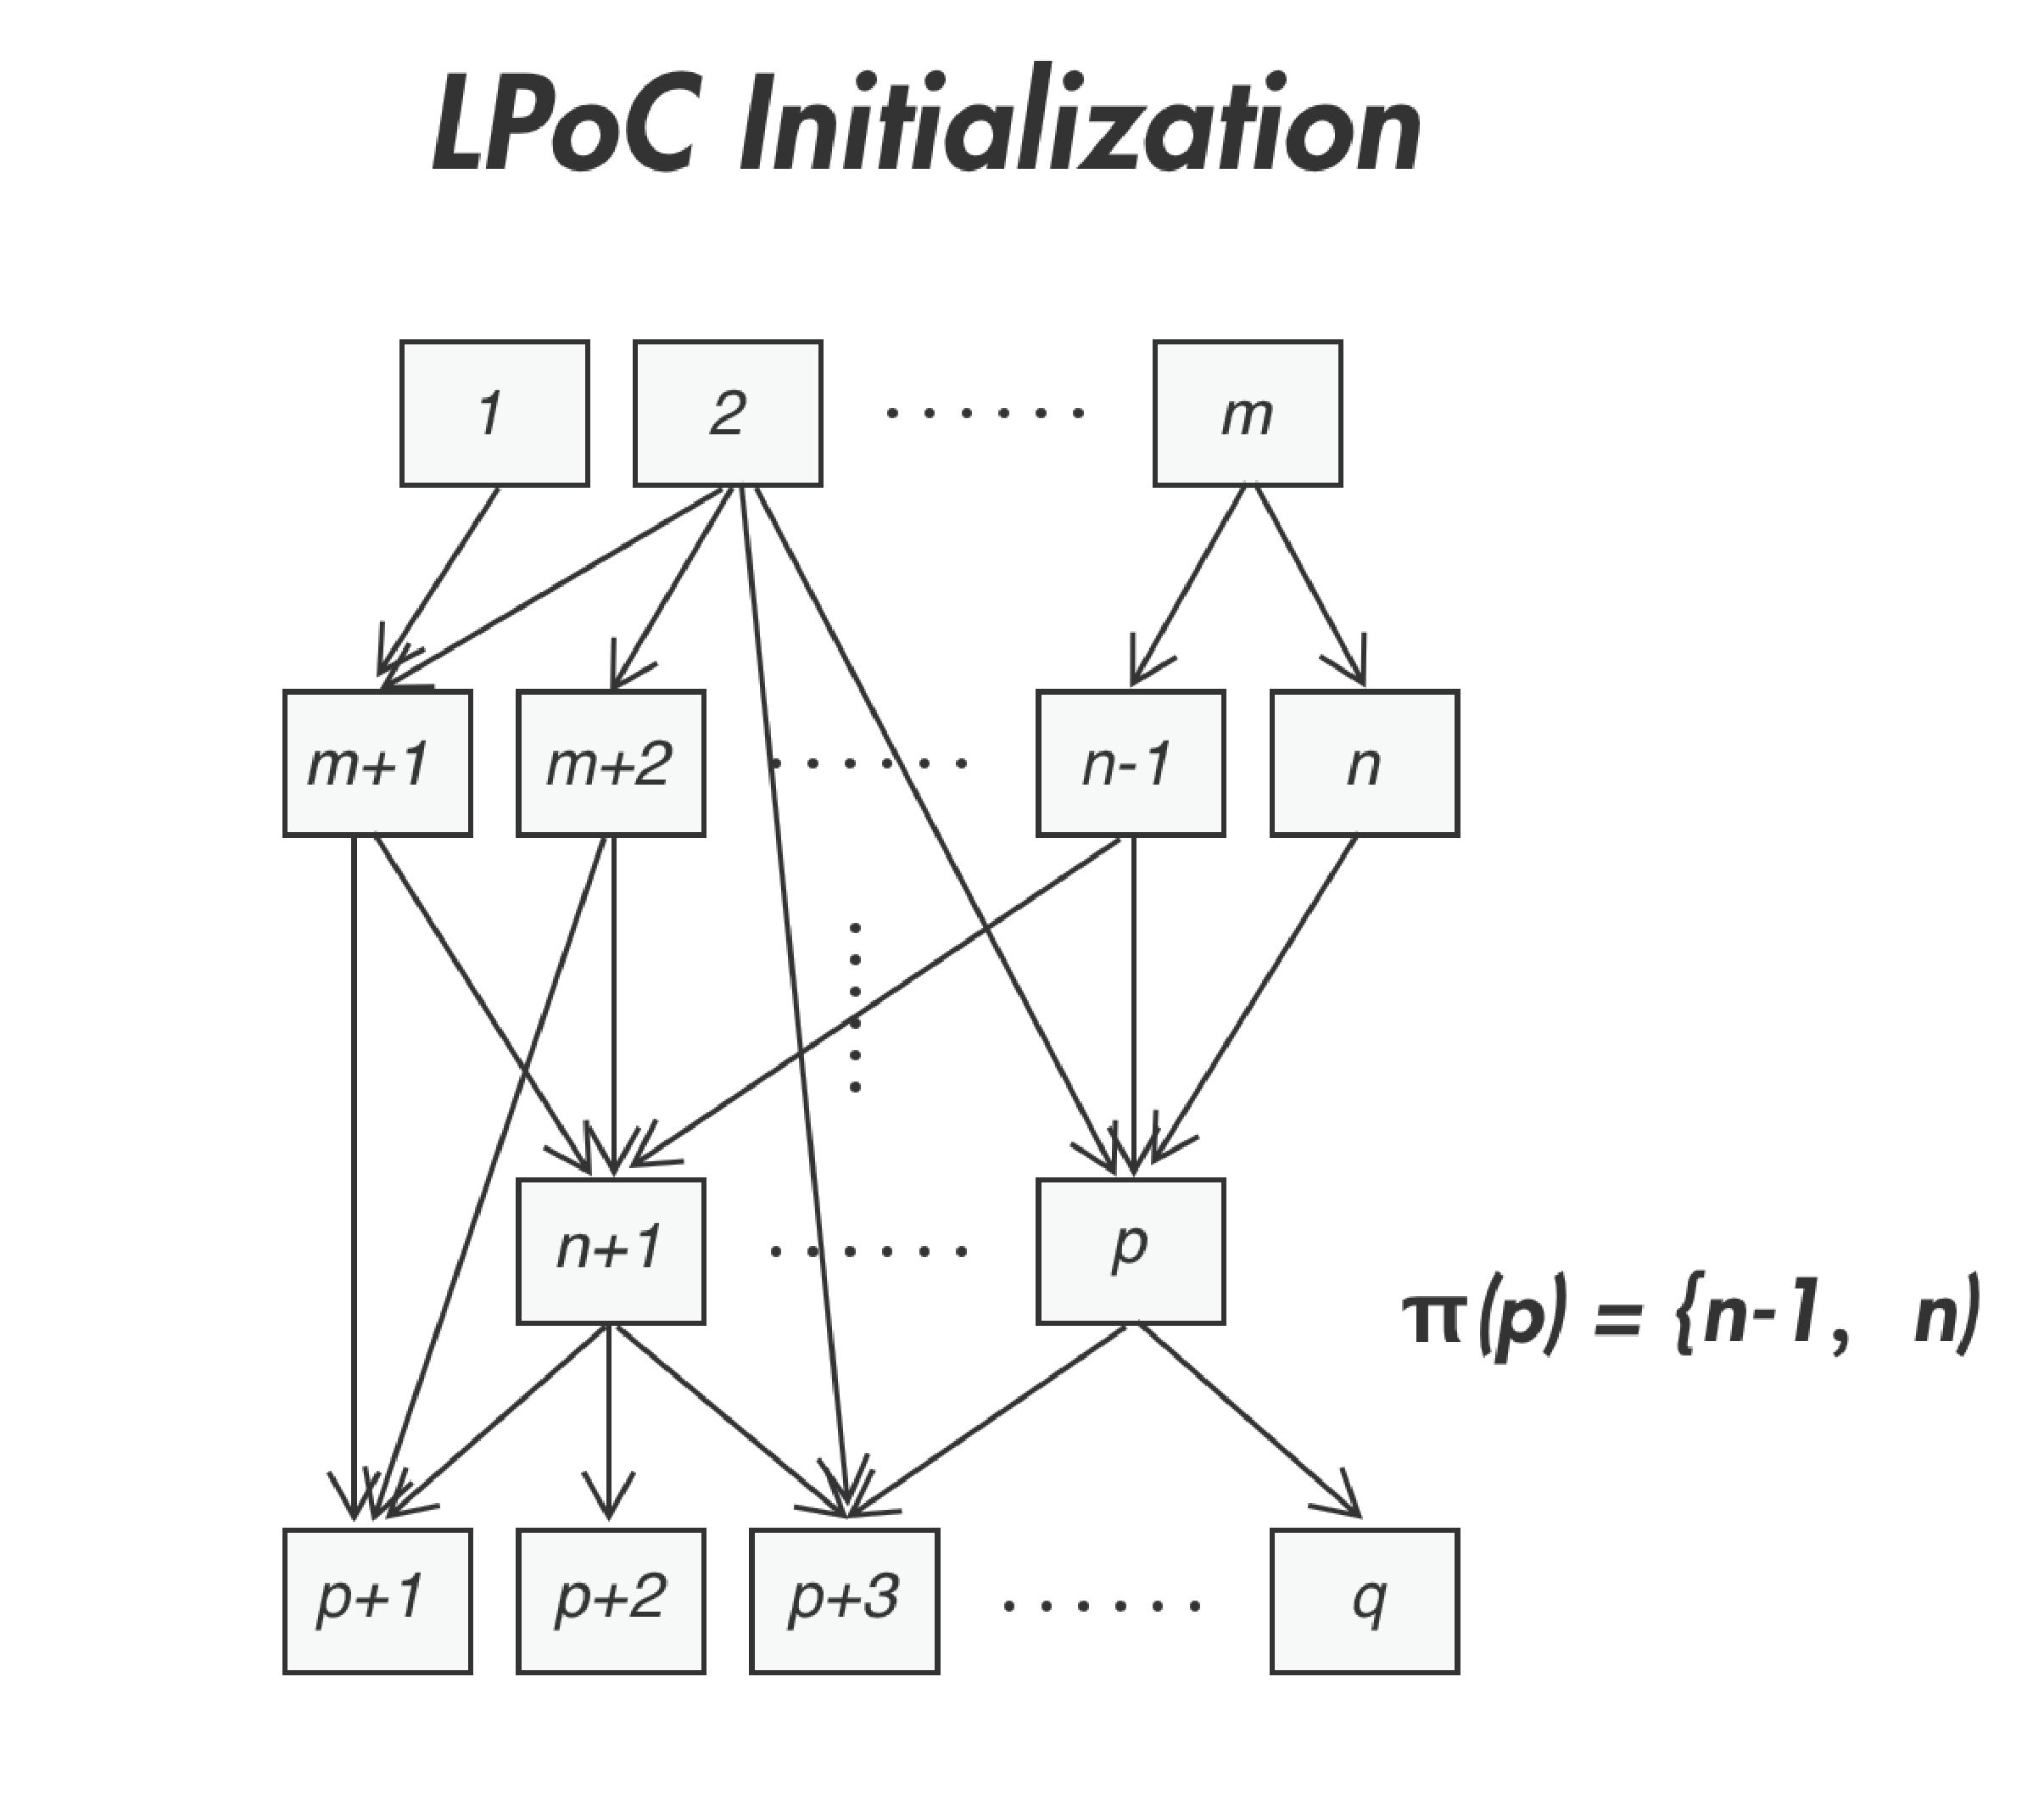
\includegraphics[width=340pt]{fig9}}
 \\ \centerline{{Figure 2.9 Initialization Phase of Light-Proof-of-Capacity}}
 \vspace{-1.5em}
\\

\hangafter 1
\hangindent 1.5em
\noindent   
1.\quad $V$ generates a unique Directed Acyclic Graph (DAG) $G=(N, E)$ for a specific miner $L$, in which N is the set of nodes in G, and E is the set of edges that connect different nodes in G.
\vspace{-0.8em}
\\

\hangafter 1
\hangindent 1.5em
\noindent   
2.\quad Let Let $\pi(n)=\{n':(n',n)\in E|n'\in N, n\in N\}$ be the set of predecessors of node $n$ in $G$.
\vspace{-0.8em}
\\

\hangafter 1
\hangindent 1.5em
\noindent   
3.\quad Let $L_{ID}$ be the identifier of $L$, let $|n|$ be the identifier of node $n$.
\vspace{-0.8em}
\\

\hangafter 1
\hangindent 1.7em
\noindent   
4.\quad Let $w(n)=CRH(L_{ID}, |n|, w(\pi(n))$ be the hash value of node $n$, in which $w(\pi(n))=(w(n_{1}),...,w(n_{M}))$ and $n_{1},...n_{M} \in \pi(n)$;
\vspace{-0.8em}
\\

\hangafter 1
\hangindent 1.7em
\noindent   
5.\quad $L$ calculates the hash value $w(n)$ for all the nodes in $G$, and stores the values in its available storage, to prepare for challenges from $V$.
\vspace{-0.5em}
\\

\noindent   
 {\bf Verification Phase}\\
\centerline{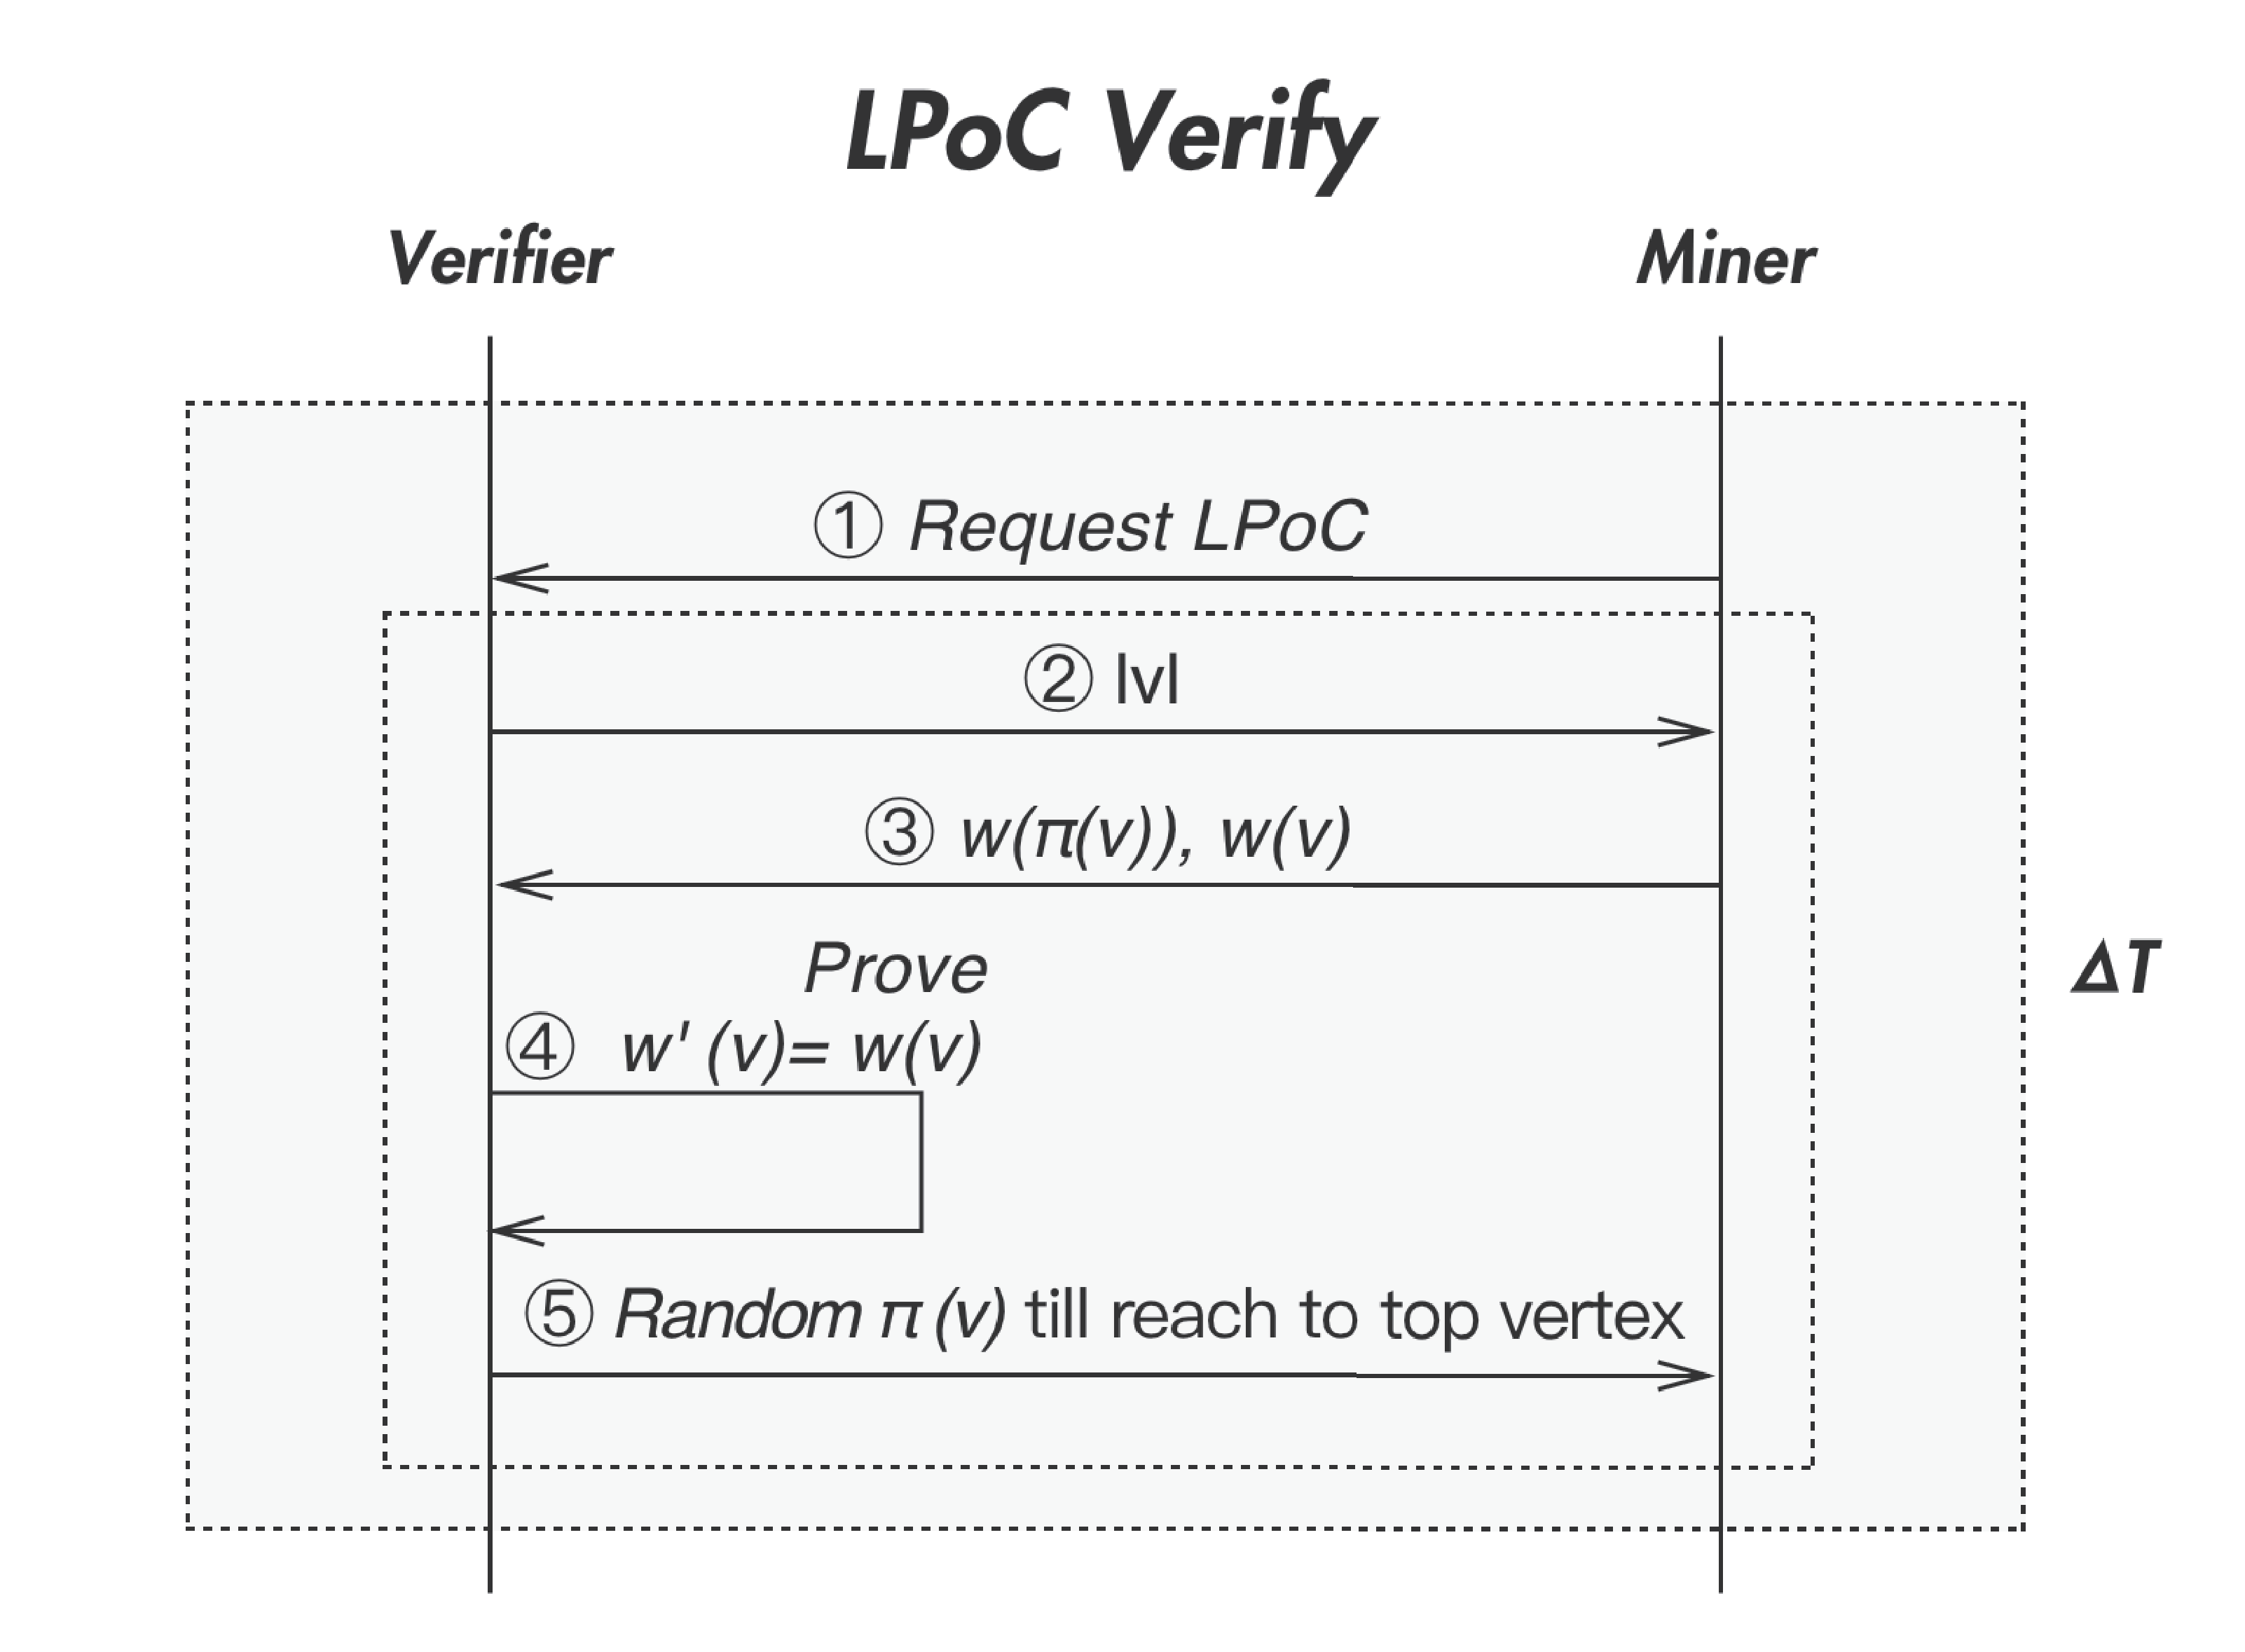
\includegraphics[width=315pt]{fig10}}
 \\ \centerline{{Figure 2.10 Verification Phase of Light-Proof-of-Capacity}}
 \vspace{-1.5em}
\\

\hangafter 1
\hangindent 1.5em
\noindent   
1.\quad At a given time $T$, $L$ requests LPoC challenge from $V$.
\vspace{-0.8em}
\\

\hangafter 1
\hangindent 1.5em
\noindent   
2.\quad $V$ choose a random node $n \in N$, and sends $|n|$ to $L$.
\vspace{-0.8em}
\\

\hangafter 1
\hangindent 1.5em
\noindent   
3.\quad Based on received $|n|$, $L$ sends its stored hash values $w(\pi(n))$ of all the nodes in $\pi(n)$ and stored $w(n)$ to $V$.
\vspace{-0.8em}
\\

\hangafter 1
\hangindent 1.7em
\noindent   
4.\quad From received $w(\pi(n))$, $V$ calculates $w'(n)$ by the formula $w(n)=CHR(L_{ID}, and |n|, w(\pi(n))$, and verifies that $w'(n)$ is identical to previously received $w(n)$ from $L$. If not, the proof has failed.
\vspace{-0.8em}
\\

\hangafter 1
\hangindent 1.8em
\noindent   
5.\quad $V$ randomly chooses one of the predecessors of $n$, repeats steps 2 to 4, until there is no more predecessors to try in any of the predecessor sets.
\vspace{-0.8em}
\\

\hangafter 1
\hangindent 1.5em
\noindent   
6.\quad Repeat the procedure from step 1 at given time intervals.
\vspace{-0.8em}
\\

\hangafter 1
\hangindent 1.9em
\noindent   
7.\quad The series of repeated successful challenges and proofs between $L$ and $V$ generates the successful proof of capacity for $L$.
 \vspace{-0.5em}

                \subsection{Consensus}%——2.4
For a decentralized blockchain network to operate, different nodes need to reach consensus to verify and record transactions in the network. It is also a required process when adding new blocks to a blockchain’s ledger. PPIO’s storage market is based on blockchain technology. It also requires a consensus mechanism explicitly designed for its storage network, to maintain a secure and healthy storage market. Commonly used consensus algorithms have their pros and cons. The Proof of Work (PoW) consensus forces each node to solve a complicated math problem, to compete to build new blocks. PoW is reliable, but it introduces meaningless computation and waste of energy. The Proof of Stake (PoS) consensus weights the nodes based on how many cryptocurrencies they hold, in deciding which node has the right to build new blocks. It enables much faster block building and alleviates the wastefulness problem in PoW, but it still runs the risk of becoming centralized, as the most prominent stakeholders are likely to dominate and become monopolies. FileCoin introduces Proof of Spacetime and uses it as a measure to calculate the power of each node in its consensus algorithm. It is a combination of the ideas behind PoW and PoS. However, using proof of spacetime alone does not adequately represent the contribution of each node. For example, certain nodes may not have a large storage capacity, but can still provide valuable download services with their high bandwidth connections, which should also be counted as the contribution to the network.
\vspace{-0.5em}
 \\ \\PPIO’s consensus algorithm takes both storage and bandwidth contribution of each miner node into account when calculating its power. The process starts by generating a pool of candidate miner nodes based on the power of each node, and from the pool, a random miner is selected via Verifiable Random Function (VRF) to build a new block. Finally, the block is validated via Byzantine Fault Tolerance (BFT) consensus. This method can improve the speed and reduce the cost of block building, prevent nodes from becoming monopolies, and maintain the consistency and security of the ledger.
\vspace{-0.5em}

                       \subsubsection{Power of Miners}  %——%2.4.1
The voting power of each node in PPIO’s network is calculated based on two factors:
\vspace{-0.8em}
\\

\hangafter 1
\hangindent 1.5em
\noindent   
•\quad  {\bf Power of Storage:} The power of storage for miner $L_{i}$ at a given time $t$ is calculated as: $L^{i,t}_{s} = \alpha * L^{i,t}_{st} / N_{st} + \beta * L^{i,t}_{c} / N_{c}$, where $L^{i,t}_{st}$ is the proven storage spacetime of miner $L_{i}$ at time $t$,  $L^{i,t}_{c}$ is its proven capacity at time $t$,  $N_{st}$ is the total proven spacetime of the entire network, and $N_{c}$ is the total proven capacity of the entire network. The calculation takes into account both the current storage spacetime and the remaining capacity of the miner so that it evaluates not only the miner’s current contribution but also its potential contribution in the future. The parameters $\alpha$ and $\beta$ can be used to adjust the balance between the two factors at the different development stages, to provide enough incentives for new miners to join and contribute resources. For example, during the early stage of the network when there is not enough data to be stored, larger $\beta$ and smaller $\alpha$ values can be used. As storage usage increases, the value of $\beta$ will be gradually decreased while the value of $\alpha$ will be gradually increased.
\vspace{-0.8em}
\\

\hangafter 1
\hangindent 1.5em
\noindent   
•\quad {\bf Power of bandwidth:} The power of bandwidth for miner $L_{i}$ at a given time $t$ is calculated as: $L^{i,t}_{b} = \gamma * L^{i,t}_{bw} / N_{bw}$, where $L^{i,t}_{bw}$ is the proven bandwidth of miner $L_{i}$ at a given time $t$, and $N_{bw}$ is the total proven bandwidth of the network.
\vspace{-0.8em}
\\

\noindent 
By combining the power of storage and the power of bandwidth, the overall power of miner $L_{i}$ at time $t$ can be calculated as: $L^{i,t}_{pow} = L^{i,t}_{s} + L^{i,t}_{b}$.
\vspace{-0.5em}
 \\ \\The next step is to apply the overall power of each node in selecting the candidates to build the next block. At time $t$, let $B_{prev}$ be the previous block in the ledger, let $M$ be the maximal value of the $Hash$ function, let $D$ be the difficulty parameter, the miners that satisfy the following condition will be selected as candidates:  $Hash(Hash(B_{prev}), L_{i}) \leq L^{i,t}_{pow}*M/D$.
 \vspace{-0.5em}
\\ \\From the equation it is clear that the chance of a miner getting selected depends on its overall power at the time $L^{i,t}_{pow}$, that represents its overall contribution to the network. Higher power leads to higher chances of being selected. 
\vspace{-0.5em}

                   
        \subsubsection{Verifiable Random Function (VRF)}  %——2.4.2\cite{article20}
 \noindent 
After the selection in 2.4.1 is complete, all the candidate miners are placed in a pool, ready for the next stage of selection. PPIO injects randomness at this step to avoid the monopoly by a small number of miners. However, in a decentralized network, randomness itself needs to be verified. Therefore PPIO adopts Verifiable Random Function (VRF) \cite{article20} in the calculation to decide which candidate miner has the final right to write a block.
\vspace{-0.5em}
\\

\noindent  
VRF is a pseudo-random function that provides publicly verifiable proofs of its outputs' correctness \cite{article24}, 
 its mathematical definition \cite{article25} is:
 \vspace{-0.8em}
\\

\hangafter 1
\hangindent 1.5em
\noindent   
•\quad $Function$ $F$
\\
\hangafter 1
\hangindent 1.5em
\noindent   
•\quad $GEN\left(1^k\right)=generates\left(PK, SK\right)$
\\
\hangafter 1
\hangindent 1.5em
\noindent   
•\quad$PROVE_{SK}(x)=(F_{SK}(x), \Pi_{SK}(x))$
\\
\hangafter 1
\hangindent 1.5em
\noindent   
•\quad $VER_{PK}(x, y, \Pi)= true \mathbin{/} false$
\vspace{-0.5em}
\\

\noindent   
Function $GEN$ generates a public key $PK$ and a private key $SK$. Apply VRF $F$ with $PK$ on input $x$ to get $y=F_{SK}(x)$ and proof $\Pi_{SK}(x)$. $y$ is the generated random number, and it can be verified using the public key $PK$ by $VER_{PK}(x, y, \Pi)= true \mathbin{/} false$.
\vspace{-0.5em}
\\ \\VRF has the following characteristics:
\vspace{-0.8em}
\\

\hangafter 1
\hangindent 1.5em
\noindent   
•\quad {\bf Uniqueness }
\vspace{-0.8em}
\\ \\$\nexists((x, y_{1}, \Pi_{1}), (x, y_{2}, \Pi_{2}))$ s.t. $VER_{PK}(x, y_{1}, \Pi_{1})=VER_{PK}(x, y_{2}, \Pi_{2})$
\vspace{-0.8em}
\\

\hangafter 1
\hangindent 1.5em
\noindent   
•\quad {\bf Provability }
\vspace{-0.8em}
\\ \\if $(y, \Pi)=PROVE_{SK}(x)$ then $VER_{PK}(x, y, \Pi)= true$
\vspace{-0.7em}
        \subsubsection{Byzantine Fault Tolerance (BFT)}  %——2.4.3
Byzantine Fault Tolerance(BFT) is originated from the Byzantine Generals' Problem, which is a famous example of distributed consensus. [21] In a distributed network, different nodes reach consensus by exchanging information. However, some messages may contain incorrect or confusing information due to node failure, or message corruption during transmission. It's also possible that certain nodes are malicious or compromised and attack the network deliberately. As a result, the consistent consensus cannot be easily achieved.  The goal of BFT is to solve these problems.
\vspace{-0.5em}
        \subsubsection{PVFT Consensus}  %——2.4.4
PPIO combines node selection based on power, randomized block building based on VRF and fault tolerance based on BFT into a unique consensus algorithm called PVFT, and its mathematical form is defined as follows:      
\vspace{-0.8em}
\\

\hangafter 1
\hangindent 1.5em
\noindent   
•\quad $G_{bp}={bp_{1}, bp_{2},...bp_{n}|stake(bp_{i})\geqslant C}$ The power of each candidate node in the candidate pool $G_{bp}$ needs to be higher or equal to a minimal value C.
\vspace{-0.8em}
\\

\hangafter 1
\hangindent 1.5em
\noindent   
•\quad $(F_{SK}(Block_{prev}), \Pi_{SK}(x)),BP=F_{SK}(Block_{prev}) \mod |G_{bp}|$. Find a random number by applying VRF to the hash of the previous block, then calculate its modulo over the size of the candidate group $G_{bp}$, and use the result to select the node to build the next block.
\vspace{-0.8em}
\\

\hangafter 1
\hangindent 1.5em
\noindent   
•\quad $BFT(G_{bp})$ Candidate nodes validate the new block being added and reach the final confirmation.
\vspace{-0.5em}

    \section{Architecture} %——3
PPIO follows a layered system design, to facilitate future expansion, and make it more friendly to developers. As shown in Figure 3.1, PPIO consists of seven layers, which are:
\vspace{-0.5em}
 \\


\hangafter 1
\hangindent 1.5em
\noindent   
1.\quad  Physical Layer: the hardware layer, that provides underlying storage and bandwidth resources, discussed in 3.1.
\vspace{-0.8em}
\\


\hangafter 1
\hangindent 1.5em
\noindent   
2.\quad Data Layer: basic data units and structures, discussed in 3.2.
\vspace{-0.8em}
\\


\hangafter 1
\hangindent 1.5em
\noindent   
3.\quad Network Layer: P2P network protocol and algorithms for connection, data transfer, load balancing and encryption, discussed in 3.3.
\vspace{-0.8em}
\\

\hangafter 1
\hangindent 1.5em
\noindent   
4.\quad Consensus Layer: PPIO’s consensus scheme and its implementation, discussed in 3.4.
\vspace{-0.8em}
\\

\hangafter 1
\hangindent 1.5em
\noindent   
5.\quad Incentive Layer: manages incentives and rewards based on the role of each node in the network, discussed in 3.5.
\vspace{-0.8em}
\\

\hangafter 1
\hangindent 1.5em
\noindent   
6.\quad Interface Layer: SDK and APIs for the developers and to support the application layer, discussed in 3.6.
\vspace{-0.8em}
\\

\hangafter 1
\hangindent 1.5em
\noindent   
7.\quad Application Layer: Apps or DApps developed by the 3rd party developers, discussed in 3.7.
\vspace{-0.3em}
 \\ \\
\centerline{\includegraphics[width=315pt]{fig11}}
\vspace{-1.5em}
\\\\
 \centerline{{Figure 3.1 The 7 layer architecture of PPIO}}
\vspace{-1.5em}
     \subsection{Physical Layer} %——3.1
Disk storage and network bandwidth are the core components of PPIO’s physical layer. They are the essential resources in PPIO’s storage network and therefore are also the basis in evaluating each storage miner’s contribution to the network. The miners with large storage capacity but limited bandwidth can contribute more in providing storage service, while with less storage but higher bandwidth can contribute more in providing bandwidth service. The miners with abundant storage and high bandwidth contribute to the network the most and in turn, get rewarded the most.
\vspace{-0.8em}
\\

\hangafter 1
\hangindent 1.5em
\noindent   
•\quad  {\bf Storage}: Physical storage may consist of Flash drive, Solid State Drive (SSD), Hard Disk Drive (HDD), Tape and Optical Disc (OD). In PPIO’s storage network, different types of storage can play different roles based on their characteristics. For example, SSD can be used to store and provide fast retrieval service for popular content. The lifespan of the storage media also needs to accommodate the length of the storage contract, for example, tape and optical disk can be used for long time storage while SSD and Flash can cover short-term storage uses.
\vspace{-0.8em}
\\

\hangafter 1
\hangindent 1.5em
\noindent   
•\quad {\bf Network bandwidth}: In bit/per second, network bandwidth measures the maximum rate of data transfer across a given network path. Network transmission media can include coaxial cable, twisted pair cable, optical fiber cable, and wireless connection. Their bandwidth varies a lot, from Kilobits and Megabits per second to Gigabits per second. Network service can be categorized into business and residential networks, and they have very different characteristics in bandwidth usage. For example, the use of business bandwidth is usually high during the day, while the use of residential bandwidth stays low. The opposite happens during night time and weekends. PPIO’s distributed storage network adapts to these dynamics to make efficient use of the available bandwidth in the network.
\vspace{-0.5em}



        \subsection{Data Layer}  %——3.2
The next above the physical layer is the data layer. As shown in Figure 3.2, there are three types of data structures used in PPIO’s storage network:
\vspace{-1em}
\\\\
\centerline{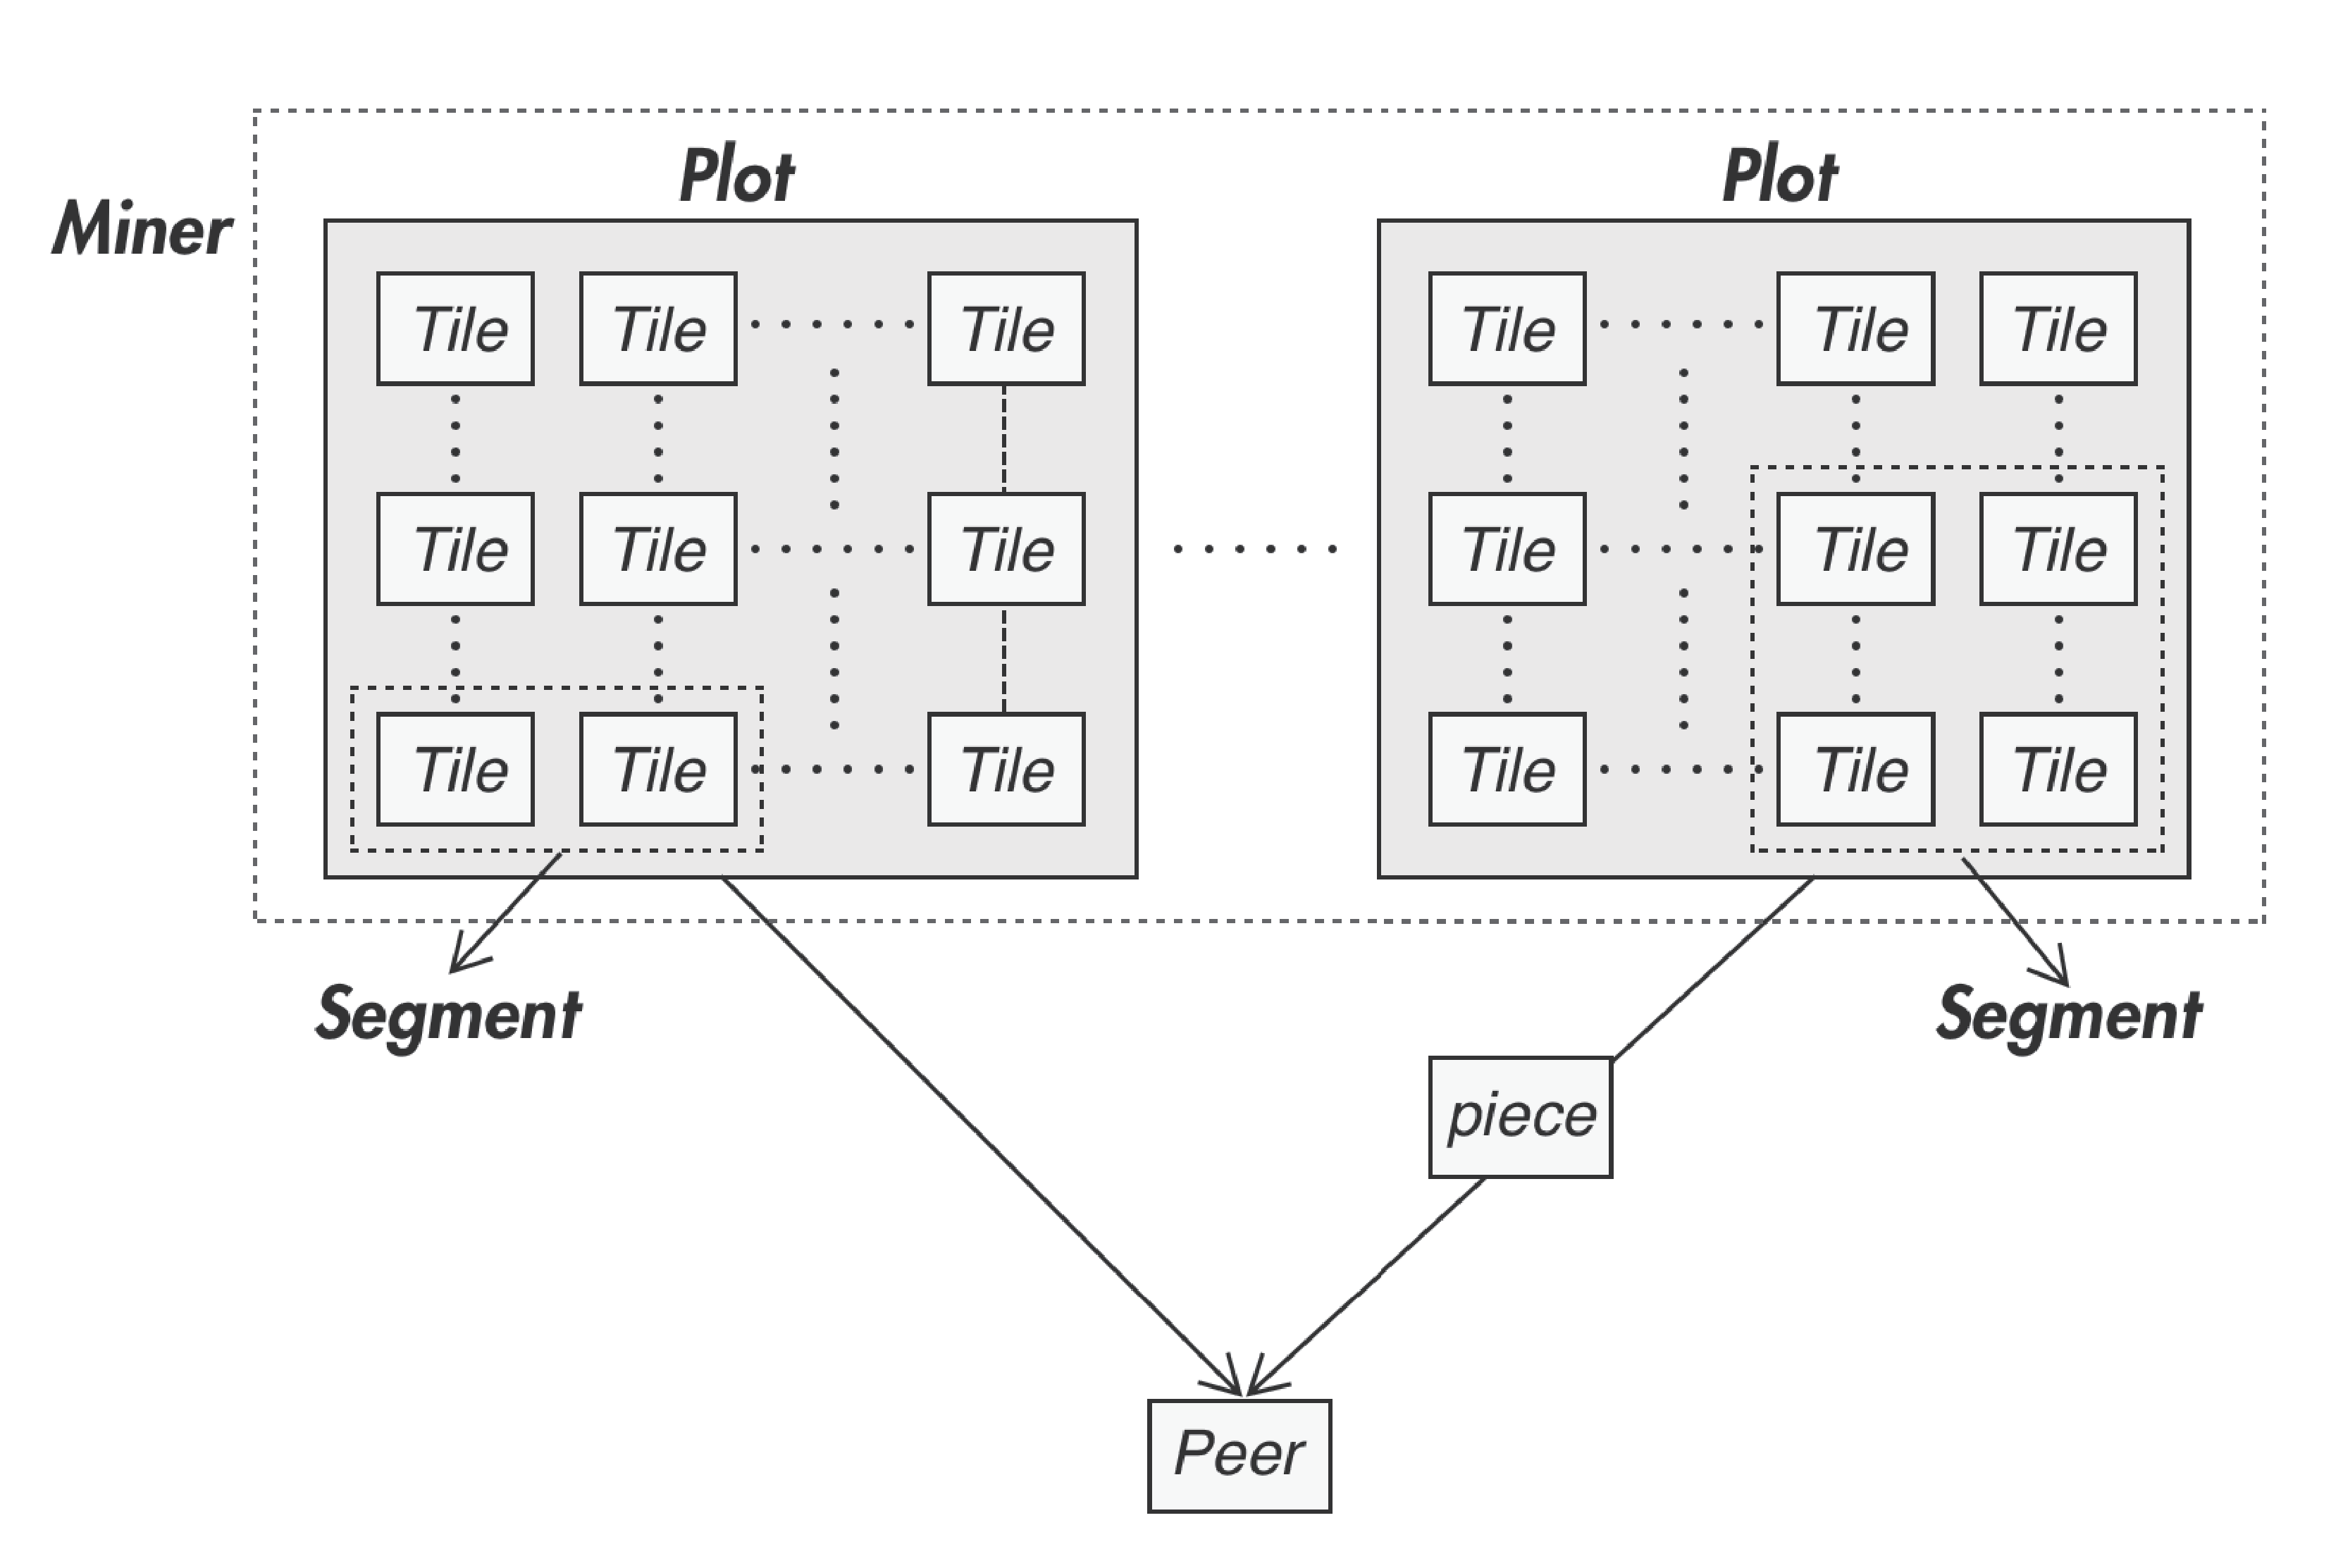
\includegraphics[width=340pt]{fig12}}
\\\\ \centerline{{Figure 3.2 The data structures in the data layer}}
\vspace{-1.5em}
\\

\hangafter 1
\noindent   
{\bf Plot /Tile: the storage capacity unit}
\vspace{-0.8em}
\\

\hangafter 1
\hangindent 1.5em
\noindent   
•\quad The Plot can be considered as a virtual drive in PPIO’s storage network, and it is initialized when the miner joins the network. Without any data stored, it's the basic unit used in capacity proof - LPoC (as described in section 2.3.4). With data stored, it is the base unit of spacetime proof - PoSt (as described in section 2.3.3).
\vspace{-0.8em}
\\

\hangafter 1
\hangindent 1.5em
\noindent   
•\quad Tile is the smallest unit of verifiable storage in the plot. Its size is 128KB. In PoRep, PoD, and PoSt, Tile is used as the basic unit in the verification.
\vspace{-0.5em}
\\

\hangafter 1
\noindent   
{\bf Segment: the storage data unit}
\vspace{-0.8em}
\\

\hangafter 1
\hangindent 1.5em
\noindent   
•\quad The segment is the base unit of PPIO’s object-oriented storage. A storage object is always divided into multiple segments. To improve privacy protection, PPIO prevents any miner node from storing all the segments of an object copy, even if the copy of the object is encrypted. A segment is also the smallest unit in storage scheduling, and its size ranges from 128KB to 16MB.
\vspace{-0.6em}
\\

\hangafter 1
\noindent   
{\bf Piece: the data transmission unit}
\vspace{-0.6em}
\\

\hangafter 1
\hangindent 1.5em
\noindent   
•\quad  A piece is the smallest data unit in PPIO’s network transmission, with the size of 128KB.
\vspace{-0.5em}
\\

\noindent  
Data redundancy is required to maintain reliable data storage. PPIO adopts two methods to add redundancy to its stored data.
\vspace{-0.6em}
\\

\hangafter 1
\noindent   
 {\bf Data Copies:} The original data is replicated into more copies. Although the method introduces large storage overhead, its computation complexity is low, and the original data can be quickly recovered. It can often be used in storing popular content.
 \vspace{-0.5em}
\\

\hangafter 1
\noindent   
{\bf Redundant Coding:} Divide the original data into blocks and encode them with Erasure Code to generate a group of new data blocks that have redundancy embedded. The original data can be recovered if no more than a certain number of the data blocks are lost or corrupted. This method has much lower storage overhead, but it is more computationally intensive. It can often be used in storing immutable or less popular content. Reed Solomon \cite{article22} is one of the commonly used Erase Code, and can be explained as follows:
%\begin{itemize}\cite{article22}
%\item 
%\end{itemize}
\vspace{-0.8em}
\\

\hangafter 1
\hangindent 1.5em
\noindent   
•\quad Let $n$ be the number of data blocks in the original data, and $m$ be the number of redundant data blocks, the original data blocks can be denoted as $D_{n \times 1}$.
\vspace{-0.8em}
\\

\hangafter 1
\hangindent 1.5em
\noindent   
•\quad Define a Distribution Matrix as $B_{(n+m) \times n}$, in which the first n rows and n columns form an identity matrix, and the remaining m rows and n columns are called Vandermonde Matrix or Cauchy Matrix.
\vspace{-0.8em}
\\

\hangafter 1
\hangindent 1.5em
\noindent   
•\quad Encoding: Encode $D_{n \times 1}$ and generate the new set of data blocks $DC_{(n+m) \times 1}$, $B_{(n+m) \times n} \times D_{n \times 1} = DC_{(n+m) \times 1}$.
\vspace{-0.8em}
\\

\hangafter 1
\hangindent 1.5em
\noindent   
•\quad Verification: Decode data blocks $B^{-1}_{n \times (n+m)} \times DC_{(n+m) \times 1} = D'_{n \times 1}$. If $D'_{n \times 1}==DC'_{n \times 1}$ data is correctly decoded, otherwise data loss or corruption has occurred, and the original data needs to be recovered.
\vspace{-0.8em}
\\

\hangindent 1.5em
\noindent   
•\quad Correction: Assume there are $m$ number of data blocks that are lost or corrupt in $DC_{(n+m) \times 1}$.
\vspace{-1em}
\\\\
- Get $DC'_{n \times 1}$ by removing m rows of corrupt data in $DC_{(n+m) \times 1}$.
\vspace{-1em}
\\\\
- Get $B'_{n \times n}$ by removing associate dispatch matrix and calculate $B'^{-1}_{n \times n}$.
\vspace{-1em}
\\\\
- Get recovered data $D_{n \times 1} = B'^{-1}_{n \times n} \times DC'_{n \times 1}$.
%\\\\$B_{(n+m) \times n} \times D_{n \times 1} = DC_{(n+m) \times 1}$
%\\ \\$B^{-1}_{n \times (n+m)} \times DC_{(n+m) \times 1} = D'_{n \times 1}$ if $D'_{n \times 1}=DC'_{n \times 1}$ data is correct, otherwise the data needs to be recovered;
%\\\\Correction: Assume there are $m$ number of data lost or corrupt in $DC_{(n+m) \times 1}$
%\\\\Get $DC'_{n \times 1}$ by removing m row of corrupt data in $DC_{(n+m) \times 1}$
%\\\\get $B'_{n \times n}$ by removing associate dispatch matrix and calculate $B'^{-1}_{n \times n}$
%\\\\get recovery data $D_{n \times 1} = B'^{-1}_{n \times n} \times DC'_{n \times 1}$
\vspace{-0.5em}


        \subsection{Network Layer}  %——3.3
Communication among different nodes in PPIO’s network is based on a set of P2P protocols that include the following:
\vspace{-0.8em}
\\

\hangafter 1
\hangindent 1.5em
\noindent   
•\quad {\bf Transmission}: Supports TCP and UDP based transmission. KCP \cite{article8}, QUIC \cite{article9} and SCTP \cite{article10} protocols can also be used, to improve efficiency and reliability.
\vspace{-0.8em}
%\cite{article10}, QUIC\cite{article11}and SCTP\cite{article12}protocols.
\\

\hangafter 1
\hangindent 1.5em
\noindent   
•\quad {\bf Connectivity}: NAT traversal technologies are essential to guarantee connectivity. PPIO utilizes STUN (Session Traversal Utilities for NAT) and network relay to help set up connections between nodes behind gateways.
\vspace{-0.8em}
\\

\hangafter 1
\hangindent 1.5em
\noindent   
•\quad {\bf Load Balance}: By using consistent hash \cite{article11}, traffic can be evenly distributed to different nodes. It helps reduce the impact of nodes leaving or new nodes joining the network.
\vspace{-0.8em}
\\

\hangafter 1
\hangindent 1.5em
\noindent   
•\quad {\bf Encryption}: By using asymmetric public-private key based signatures, and symmetric data encryption, the identity of message senders can be verified, and the content of the message can be validated.
\vspace{-0.5em}


        \subsection{Consensus Layer}  %——3.4
As described in section 2.4, PPIO’s consensus algorithm is specifically designed for its distributed storage network. It integrates the storage proofs, VRF random selection, and BFT consensus. To further improve its performance and scalability, PPIO also adopts a layered approach in its implementation of the consensus layer. Nodes in the network are grouped into many side chains and one master chain. The master chain is formed by selected nodes that are responsible for maintaining the consensus of the entire network. In each side chain, transactions are handled locally but aggregated and reported to the master chain periodically. Fig 3.3 shows an example of the layered consensus. Nodes in the P2P are grouped into 3 groups, the master group, the black side chain group and the white side chain group. The details of the design are presented below.
\vspace{-0.6em}
\\ \\
\centerline{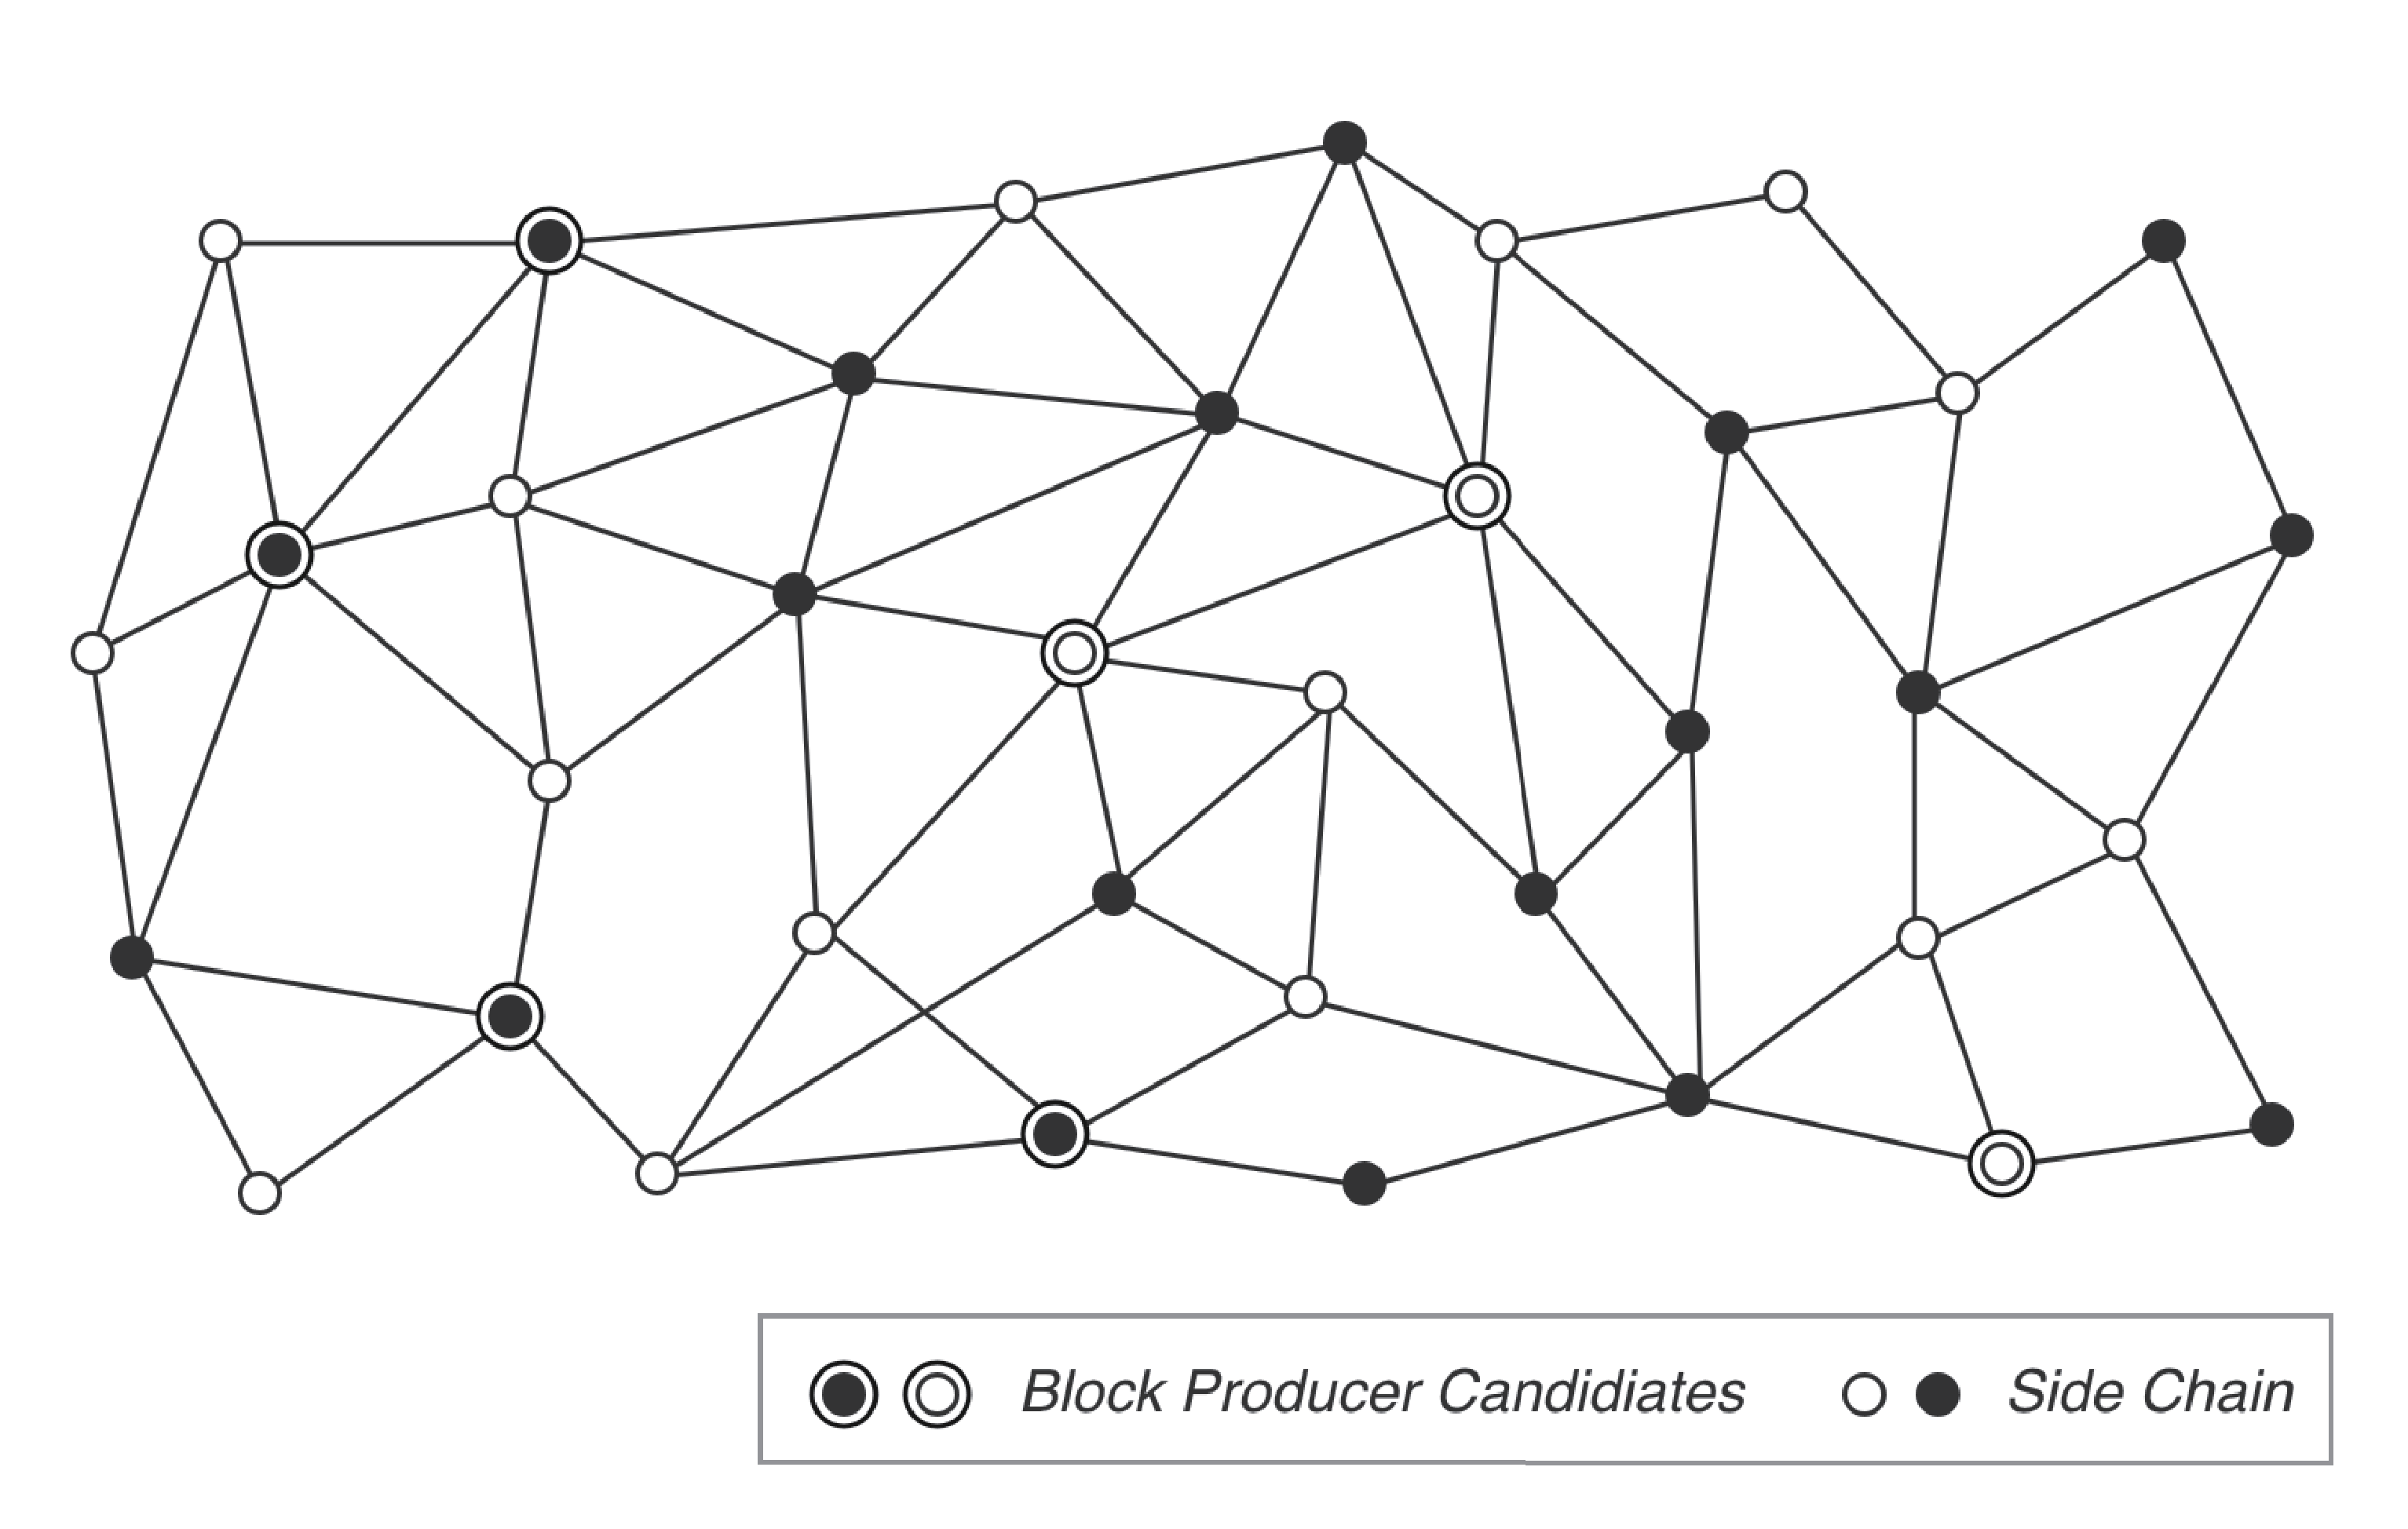
\includegraphics[width=320pt]{fig13}}
\vspace{-0.8em}
\\ \centerline{{Figure 3.3 Groups of P2P nodes}}
\vspace{-1.5em}
\\\\
\hangafter 1
\noindent   
{\bf Master Chain},nodes in the master chain apply PPIO’s consensus scheme to maintain the entire network.
\vspace{-0.8em}
\\

\hangafter 1
\hangindent 1.5em
\noindent   
•\quad Nodes are selected to join the master chain based on their storage and bandwidth contribution, once the node's contributions cross a threshold, it is allowed to join the master chain.
\vspace{-0.8em}
\\

\hangafter 1
\hangindent 1.5em
\noindent   
•\quad Each node in the master chain is also a member of a side chain, and it is responsible for recording the transactions and maintaining the ledger of the side chain.
\vspace{-0.8em}
\\

\hangafter 1
\hangindent 1.5em
\noindent   
•\quad The nodes in the master chain are also responsible for:
\vspace{-1em}
\\

\hangafter 0
\hangindent 2em
\noindent   
-\quad Creating and managing side chains.
\vspace{-1em}
\\

\hangafter 0
\hangindent 2em
\noindent   
-\quad Validating and executing storage contracts and transactions.
\vspace{-1em}
\\

\hangafter 0
\hangindent 2em
\noindent   
-\quad Maintaining the ledger of the master chain.
\vspace{-0.6em}
\\

\hangafter 1
\noindent   
 {\bf Side Chain}: 
 \vspace{-0.8em}
 \\

\hangafter 1
\hangindent 1.5em
\noindent   
•\quad A newly joined node is assigned to a side chain based on network distance and load balancing, to maintain high-speed connections among the nodes in the same side chain. At least one of the nodes in the master chain needs to be allocated to each side chain.
\vspace{-0.8em}
\\

\hangafter 1
\hangindent 1.5em
\noindent   
•\quad Nodes can switch chains to adapt to changes in the network. Side chains with few nodes in it can be combined with other chains. 
\vspace{-0.8em}
\\

\hangafter 1
\hangindent 1.5em
\noindent   
•\quad Nodes in the side chain are responsible for:
\vspace{-1em}
\\

\hangafter 0
\hangindent 2em
\noindent   
-\quad Handling storage operations.
\vspace{-1em}
\\

\hangafter 0
\hangindent 2em
\noindent   
-\quad Conducting storage proofs including PoRep, PoD, PoSt and LPoC.
\vspace{-1em}
\\

\hangafter 0
\hangindent 2em
\noindent   
-\quad Matching storage contracts between miners and users.
\vspace{-1em}
\\

\hangafter 0
\hangindent 2em
\noindent   
-\quad Maintaining the ledger of the side chain.
\vspace{-1em}
\\

\hangafter 0
\hangindent 2em
\noindent   
-\quad Reporting proofs and matched contracts to the master chain.
\vspace{-0.8em}
\\

\noindent
{\bf Advantages of layered consensus}:
\vspace{-0.8em}
\\

\hangafter 1
\hangindent 1.5em
\noindent   
•\quad In a decentralized storage network, nodes take on many different roles and every operation needs to be verified. Layered consensus helps simplify the management of network nodes and avoids the inefficiency of having to sync through the entire network.
\vspace{-0.8em}
\\

\hangafter 1
\hangindent 1.5em
\noindent   
•\quad Maintaining low network latency is the key to meet user’s high expectations on storage and download performance. Layered consensus allows the network to be partitioned based on network distance and connection speed. As the storage operations can be handled within each side chain, low latency can be achieved.
\vspace{-0.8em}
\\

\hangafter 1
\hangindent 1.5em
\noindent   
•\quad Storage or download of each object requires a contract. The contracts need to validated, matched, executed, and then recorded in the ledger. Doing all these on a single chain can overload the network. With the layered approach, the side chain can take over part of the workload, and it allows the network to scale better and be able to handle large quantities of concurrent transactions.
\vspace{-0.5em}

        \subsection{Incentive Layer}  %——3.5
The foundation of PPIO’s incentive mechanism is formed by the various proofs described in 2.3, including PoRep, PoD, PoSt, and LPoC. These proofs are strictly derived and rigorously tested, to enable reliable verification of different types of work done by the nodes in the network, so that the right amount of reward can be given to different parties, to maintain a healthy economy and keep it growing.
\vspace{-0.5em}
\\ \\  The smart contract is the basis of PPIO’s reward mechanism:
\vspace{-0.5em}
\\

\hangafter 1
\noindent   
  {\bf Storage Contract }: 
  \vspace{-0.8em}
\\

\hangafter 1
\hangindent 1.5em
\noindent   
•\quad  {\bf User storage contract:} User creates a storage contract to store files to the network, which includes information about the storage object, storage duration, number of copies and the amount of payment offered.
  \vspace{-0.8em}
\\

\hangafter 1
\hangindent 1.5em
\noindent   
•\quad  {\bf Miner storage contract:} Miner submits storage contract to offer storage service, which includes information about its storage capacity, available duration, amount of acceptable payment. The miner storage contract can also be updated later on.
  \vspace{-0.8em}
\\

\hangafter 1
\hangindent 1.5em
\noindent   
•\quad The indexer matches user's and miner’s contracts. When successful, User starts to upload copies of the object to miners. All data transfer is scheduled by the indexer.
  \vspace{-0.5em}
\\

\hangafter 1
\noindent   
 {\bf Download Contract }: 
   \vspace{-0.8em}
\\

\hangafter 1
\hangindent 1.5em
\noindent   
•\quad  {\bf User download contract:} User creates download contract to download files, which includes information about the object to be downloaded and the amount of payment offered.
  \vspace{-0.8em}
\\

\hangafter 1
\hangindent 1.5em
\noindent   
•\quad  {\bf Miner download contract:} Miner submits download contract to offer download services, which includes information about the bandwidth provided, duration and amount of acceptable payment.
  \vspace{-0.8em}
\\

\hangafter 1
\hangindent 1.5em
\noindent   
•\quad The indexer tries to match the user’s and miner’s contracts. When successful, User starts to download the object from miners. All data transfer is scheduled by the indexer.
  \vspace{-0.5em}
\\


\noindent   
In PPIO’s network, different nodes are getting rewarded based on their roles:
  \vspace{-0.8em}
\\

\hangafter 1
\hangindent 1.5em
\noindent   
•\quad {\bf Indexer}: When user download or store data, it needs to obtain indexing info from the Indexers. Therefore the Indexers receive indexing reward. When the Indexers dispatch tasks to the miners,  they also receive scheduling reward.  
  \vspace{-0.8em}
\\

\hangafter 1
\hangindent 1.5em
\noindent   
•\quad  {\bf Verifier}: The Verifiers conduct all of the storage proofs PoRep, PoD, PoSt, and PoC, and they receive verification reward.
  \vspace{-0.8em}
\\

\hangafter 1
\hangindent 1.5em
\noindent   
•\quad  {\bf Miner}: The miners not only provide storage space to store user data but also provide network bandwidth to enable data transfer. The consumption of storage and network bandwidth will be compensated accordingly. At the same time, based on the amount of storage and bandwidth the miners contribute to the network, they will receive rewards periodically.
  \vspace{-0.8em}
\\

\hangafter 1
\hangindent 1.5em
\noindent   
•\quad  {\bf Block Builder}: The nodes that record transactions and maintain the ledger get rewarded by receiving a portion of the transaction fees. They also receive a reward for adding a new block to the ledger.
  \vspace{-0.5em}

     
        \subsection{Interface Layer}  %——3.6
One of core design goals of PPiO is to provide programmable distributed storage, that can also be called Decentralized Storage as a Service (DSaaS), To be more friendly to developers, it provides: \\
  \vspace{-0.5em}

\hangafter 1
\noindent   
{\bf SDK}
  \vspace{-0.8em}
\\\\It provides high-level APIs on various platforms, such as iOS, Android, Mac and Windows.
  \vspace{-0.5em}
\\

\hangafter 1
\noindent   
{\bf Web API}
  \vspace{-0.8em}
\\\\Facilitates the developers to develop web-based applications.
  \vspace{-0.5em}
\\

\hangafter 1
\noindent   
{\bf JSON-RPC interface}
  \vspace{-0.8em}
\\\\Allows DApps to make calls to functionalities on the distributed nodes, enable easy integration of PPIO’s storage system.
  \vspace{-0.5em}
\\

\hangafter 1
\noindent     
 {\bf App sandbox}
   \vspace{-0.8em}
\\\\
PPIO can support a large number of applications running concurrently in its storage network. Developers can configure the security of the files in their applications.
  \vspace{-0.8em}
\\

\hangafter 1
\hangindent 1.5em
\noindent   
•\quad Each App has its own encryption key.
  \vspace{-0.6em}
\\

\hangafter 0
\hangindent 1.5em
\noindent   
-\quad App developers can specify how to encrypt data objects in their applications:
  \vspace{-1em}
\\

\hangafter 0
\hangindent 3.5em
\noindent   
-\quad Encryption using the encryption key of the App only.
  \vspace{-1em}
\\

\hangafter 0
\hangindent 3.5em
\noindent   
-\quad Encryption using the encryption keys of both the App and the user.  
  \vspace{-1em}
\\

\hangafter 0
\hangindent 1.5em
\noindent   
-\quad The owner of an object can configure the object access in three ways:
  \vspace{-1em}
\\

\hangafter 0
\hangindent 3.5em
\noindent   
-\quad Private: only the owner can access.
  \vspace{-1em}
\\

\hangafter 0
\hangindent 3.5em
\noindent   
-\quad Sharable: the owner can share the access to the object to some other users.
  \vspace{-1em}
\\

\hangafter 0
\hangindent 3.5em
\noindent   
-\quad Public: all users can access the object.
  \vspace{-1em}
\\

\hangafter 0
\hangindent 3.5em
\noindent   
-\quad App developers are responsible for the content of the files in their applications.
  \vspace{-0.5em}
\\

\noindent  
\centerline{\includegraphics[width=360pt]{fig14}}
\\\\ \centerline{{ Figure 3.4 Diagram of App sandbox}}%——名称待确认
  \vspace{-0.5em}
\\
 
\noindent  
PPIO provides two levels of APIs. The low-level APIs grant developers more flexibility and finer control over PPIO’s various functionalities. The high-level interfaces are more straightforward, and they work as traditional file systems by design to enable fast and easy adoption.
  \vspace{-0.5em}
\\

\hangafter 1
\hangindent 1.5em
\noindent   
•\quad{\bf Low-level APIs}
  \vspace{-0.8em}
\\

\hangafter 0
\hangindent 1.5em
\noindent   
-\quad {\bf PPIO-user init}: initialize user node.
  \vspace{-0.8em}
\\

\hangafter 0
\hangindent 1.5em
\noindent   
-\quad {\bf PPIO-user bucket...}: bucket related operations such as creation, deletion, etc.
  \vspace{-0.8em}
\\

\hangafter 0
\hangindent 1.5em
\noindent   
-\quad {\bf PPIO-user object...}: object related operations such as creation, deletion, etc.
  \vspace{-0.8em}
\\

\hangafter 0
\hangindent 1.5em
\noindent   
-\quad {\bf PPIO-user metadata...}: metadata related operations.
  \vspace{-0.8em}
\\

\hangafter 0
\hangindent 1.5em
\noindent   
-\quad {\bf PPIO-user storage gc}: delete data that no loner has a storage contract.
  \vspace{-0.8em}
\\

\hangafter 0
\hangindent 1.5em
\noindent   
-\quad {\bf PPIO-user storage usage}: list the usage info of the storage.
  \vspace{-0.8em}
\\

\hangafter 0
\hangindent 1.5em
\noindent   
-\quad {\bf PPIO-user daemon start}: start RPC and P2P service.
  \vspace{-0.8em}
\\

\hangafter 0
\hangindent 1.5em
\noindent   
-\quad {\bf PPIO-user daemon stop}: shutdown service.
  \vspace{-0.8em}
\\

\hangafter 0
\hangindent 1.5em
\noindent   
-\quad {\bf PPIO-user user ls}: show current user's information, such as id, ip address etc..
  \vspace{-0.8em}
\\

\hangafter 0
\hangindent 1.5em
\noindent   
-\quad {\bf PPIO-user net ping $<$peer-id$>$}: test connectivity of a peer, user or miner.
  \vspace{-0.8em}
\\

\hangafter 0
\hangindent 1.5em
\noindent   
-\quad {\bf PPIO-user net peers}: show all current peers connected.
  \vspace{-0.5em}
\\

\hangafter 1
\hangindent 1.5em
\noindent   
•\quad {\bf High-level Storage APIs}
  \vspace{-0.8em}
\\

\hangafter 0
\hangindent 1.5em
\noindent   
-\quad {\bf PPIO-ndisk init}: initlialize network disk.
  \vspace{-0.8em}
\\

\hangafter 0
\hangindent 1.5em
\noindent   
-\quad {\bf PPIO-ndisk usage}: check the usage of network disk.
  \vspace{-0.8em}
\\

\hangafter 0
\hangindent 1.5em
\noindent   
-\quad {\bf PPIO-ndisk put}: upload local file to network disk.
  \vspace{-0.8em}
\\

\hangafter 0
\hangindent 1.5em
\noindent   
-\quad {\bf PPIO-ndisk get}: download file from network disk.
  \vspace{-0.8em}
\\

\hangafter 0
\hangindent 1.5em
\noindent   
-\quad {\bf PPIO-ndisk copy}: copy file from other's network disk.
  \vspace{-0.8em}
\\

\hangafter 0
\hangindent 1.5em
\noindent   
-\quad {\bf PPIO-ndisk mkdir}: create a directory.
  \vspace{-0.8em}
\\

\hangafter 0
\hangindent 1.5em
\noindent   
-\quad {\bf PPIO-ndisk ls}: list contents of network disk.
  \vspace{-0.8em}
\\

\hangafter 0
\hangindent 1.5em
\noindent   
-\quad {\bf PPIO-ndisk cp}: copy file from network disk.
  \vspace{-0.8em}
\\

\hangafter 0
\hangindent 1.5em
\noindent   
-\quad {\bf PPIO-ndisk rm}: delete file from network disk.
  \vspace{-0.8em}
\\

\hangafter 0
\hangindent 1.5em
\noindent   
-\quad {\bf PPIO-ndisk mv}: move file on network disk.
  \vspace{-0.8em}
\\

\hangafter 0
\hangindent 1.5em
\noindent   
-\quad {\bf PPIO-ndisk assign}: grant access privilege to another user.  
  \vspace{-0.5em}
%——————————————————————————————————————————需要调整
\\

\hangafter 1
\hangindent 1.5em
\noindent   
•\quad{\bf High-level multimedia App development interface}
  \vspace{-0.8em}
\\

\hangafter 0
\hangindent 1.5em
\noindent   
-\quad {\bf PPIO-media info}: get stream media basic info
  \vspace{-0.8em}
\\

\hangafter 0
\hangindent 1.5em
\noindent   
-\quad {\bf  PPIO-media play}: start to play stream media
  \vspace{-0.8em}
\\

\hangafter 0
\hangindent 1.5em
\noindent   
-\quad {\bf PPIO-media stop}: stop to play stream media
  \vspace{-0.8em}
\\

\hangafter 0
\hangindent 1.5em
\noindent   
-\quad {\bf PPIO-media pause}: pause stream media
  \vspace{-0.8em}
\\

\hangafter 0
\hangindent 1.5em
\noindent   
-\quad{\bf PPIO-media seek}: seek to a point in the stream media and resume playing
  \vspace{-0.5em}

        \subsection{Application Layer}  %——3.7
PPIO’s APIs are designed to enable third-party developers to build all kinds of applications, including but not limited to the following:
  \vspace{-0.5em}
 \\\\{\bf Storage Application}
   \vspace{-0.8em}
\\

\hangafter 1
\hangindent 1.5em
\noindent   
•\quad Private data storage. Due to its decentralized nature, PPIO storage network is very suitable for private network storage applications. Personal data is partitioned, encrypted and stored on different nodes to ensure a high-level of privacy protection. At the same time, access to the data is restricted by the user’s private key, making personal data assets even more secure.
  \vspace{-0.8em}
\\

\hangafter 1
\hangindent 1.5em
\noindent   
•\quad Enterprise data storage: PPIO can provide significant cost savings for enterprise data storage while providing high-performance services. At the same time, its interfaces are compatible with those of the existing data storage services such as AWS S3 and make the migration to PPIO much easier.
  \vspace{-0.5em}
 \\

\noindent   
 {\bf DApps}
   \vspace{-0.6em}
\\ \\Storing application data on the blockchain is very expensive for decentralized applications. Smart contracts or other applications' data can be stored on external storage by utilizing PPIO’s APIs, to achieve significant cost saving. For example:
  \vspace{-0.8em}
\\

\hangafter 1
\hangindent 1.5em
\noindent   
•\quad Social DApps: PPIO can help validate the identity of users and their messages, it can also help to keep the conversations private.
  \vspace{-0.8em}
\\

\hangafter 1
\hangindent 1.5em
\noindent   
•\quad Ads system: Besides storing the advertisement content,  PPIO can also help accurately calculating and reporting the statistics of Ad access, such as the click-through-rate. As such data is usually the basis of ads payment, its accuracy and transparency have always been an issue for traditional ads platforms. Businesses may not be able to validate the statistics reported, to make sure they are paying for the actual exposure of the ads, and understand real user preference. PPIO can efficiently resolve these problems.
  \vspace{-0.8em}
\\

\hangafter 1
\hangindent 1.5em
\noindent   
•\quad Traceability Apps: Supply chain or other DApps that require reliable and verifiable data storage.
  \vspace{-0.5em}
\\

\noindent 
 {\bf Media  Applications}
   \vspace{-0.8em}
\\

\hangafter 0
\hangindent 1.5em
\noindent 
PPIO provides cost-effective bandwidth resource that can help reduce the cost of content distribution significantly. PPIO is also equipped with scheduling and transmission algorithms specifically optimized to achieve smooth streaming playback. Along with its PCDN caching for on-demand content distribution, and cross-network acceleration for real-time broadcasting, the high-quality user experience can be achieved and maintained for media applications. At the same time, PPIO can provide reliable statistics on content consumption that are valuable marketing data for these applications.
  \vspace{-0.5em}
\\

\noindent 
 {\bf Data Exchange}
   \vspace{-0.8em}
\\

\hangafter 0
\hangindent 1.5em
\noindent 
 File assets can be traded in PPIO’s network. PPIO can provide ways to match the sellers and buyers and handle transactions securely and reliably, without requiring an intermediate party. Commonly used applications such as app markets and content platforms can benefit from using PPIO.
    \vspace{-0.5em}
\\

\noindent 
 {\bf Data Warehouse}
    \vspace{-0.5em}
\\

\hangafter 0
\hangindent 1.5em
\noindent 
PPIO can be used as an enterprise data warehouse, to store a huge amount of historical data, and replace traditional unreliable local data storage or expensive cloud storage. Besides enterprise data, PPIO can also be used to store a public database such as a gene pool.
   \vspace{-0.5em}
\\

\noindent 
For other types of storage needs, PPIO will also provide the necessary support. Besides, PPIO will be open sourced shortly. At that time, App enthusiasts and developers will be able to participate in PPIO's development and add support for many more applications.
   \vspace{-0.5em}
   \section{Security} %——4
Maintaining security is the most critical task in a distributed storage network. PPIO’s design follows strict security measures to ensure the integrity and reliability of its storage system. This chapter discusses how PPIO defends against common network attacks, including Sybil Attacks, Outsourcing Attacks, Generation attacks that target the decentralized storage system itself, and Distributed Denial of Service (DDoS) Attacks, Eclipse Attacks that target the blockchain.
   \vspace{-0.5em}
      \subsection{Sybil Attacks} %——4.1
As shown in Figure 4.1, Sybil attack takes place when a greedy miner node creates multiple accounts in the network and claims to have stored a copy of the data in each account, but in fact, it has only stored a single copy. If successful, the attack allows the miner to receive rewards from multiple accounts unfairly. On the other hand, it can significantly reduce the actual data redundancy in the network, and severely compromise the reliability of the storage system.
\\\\ \centerline{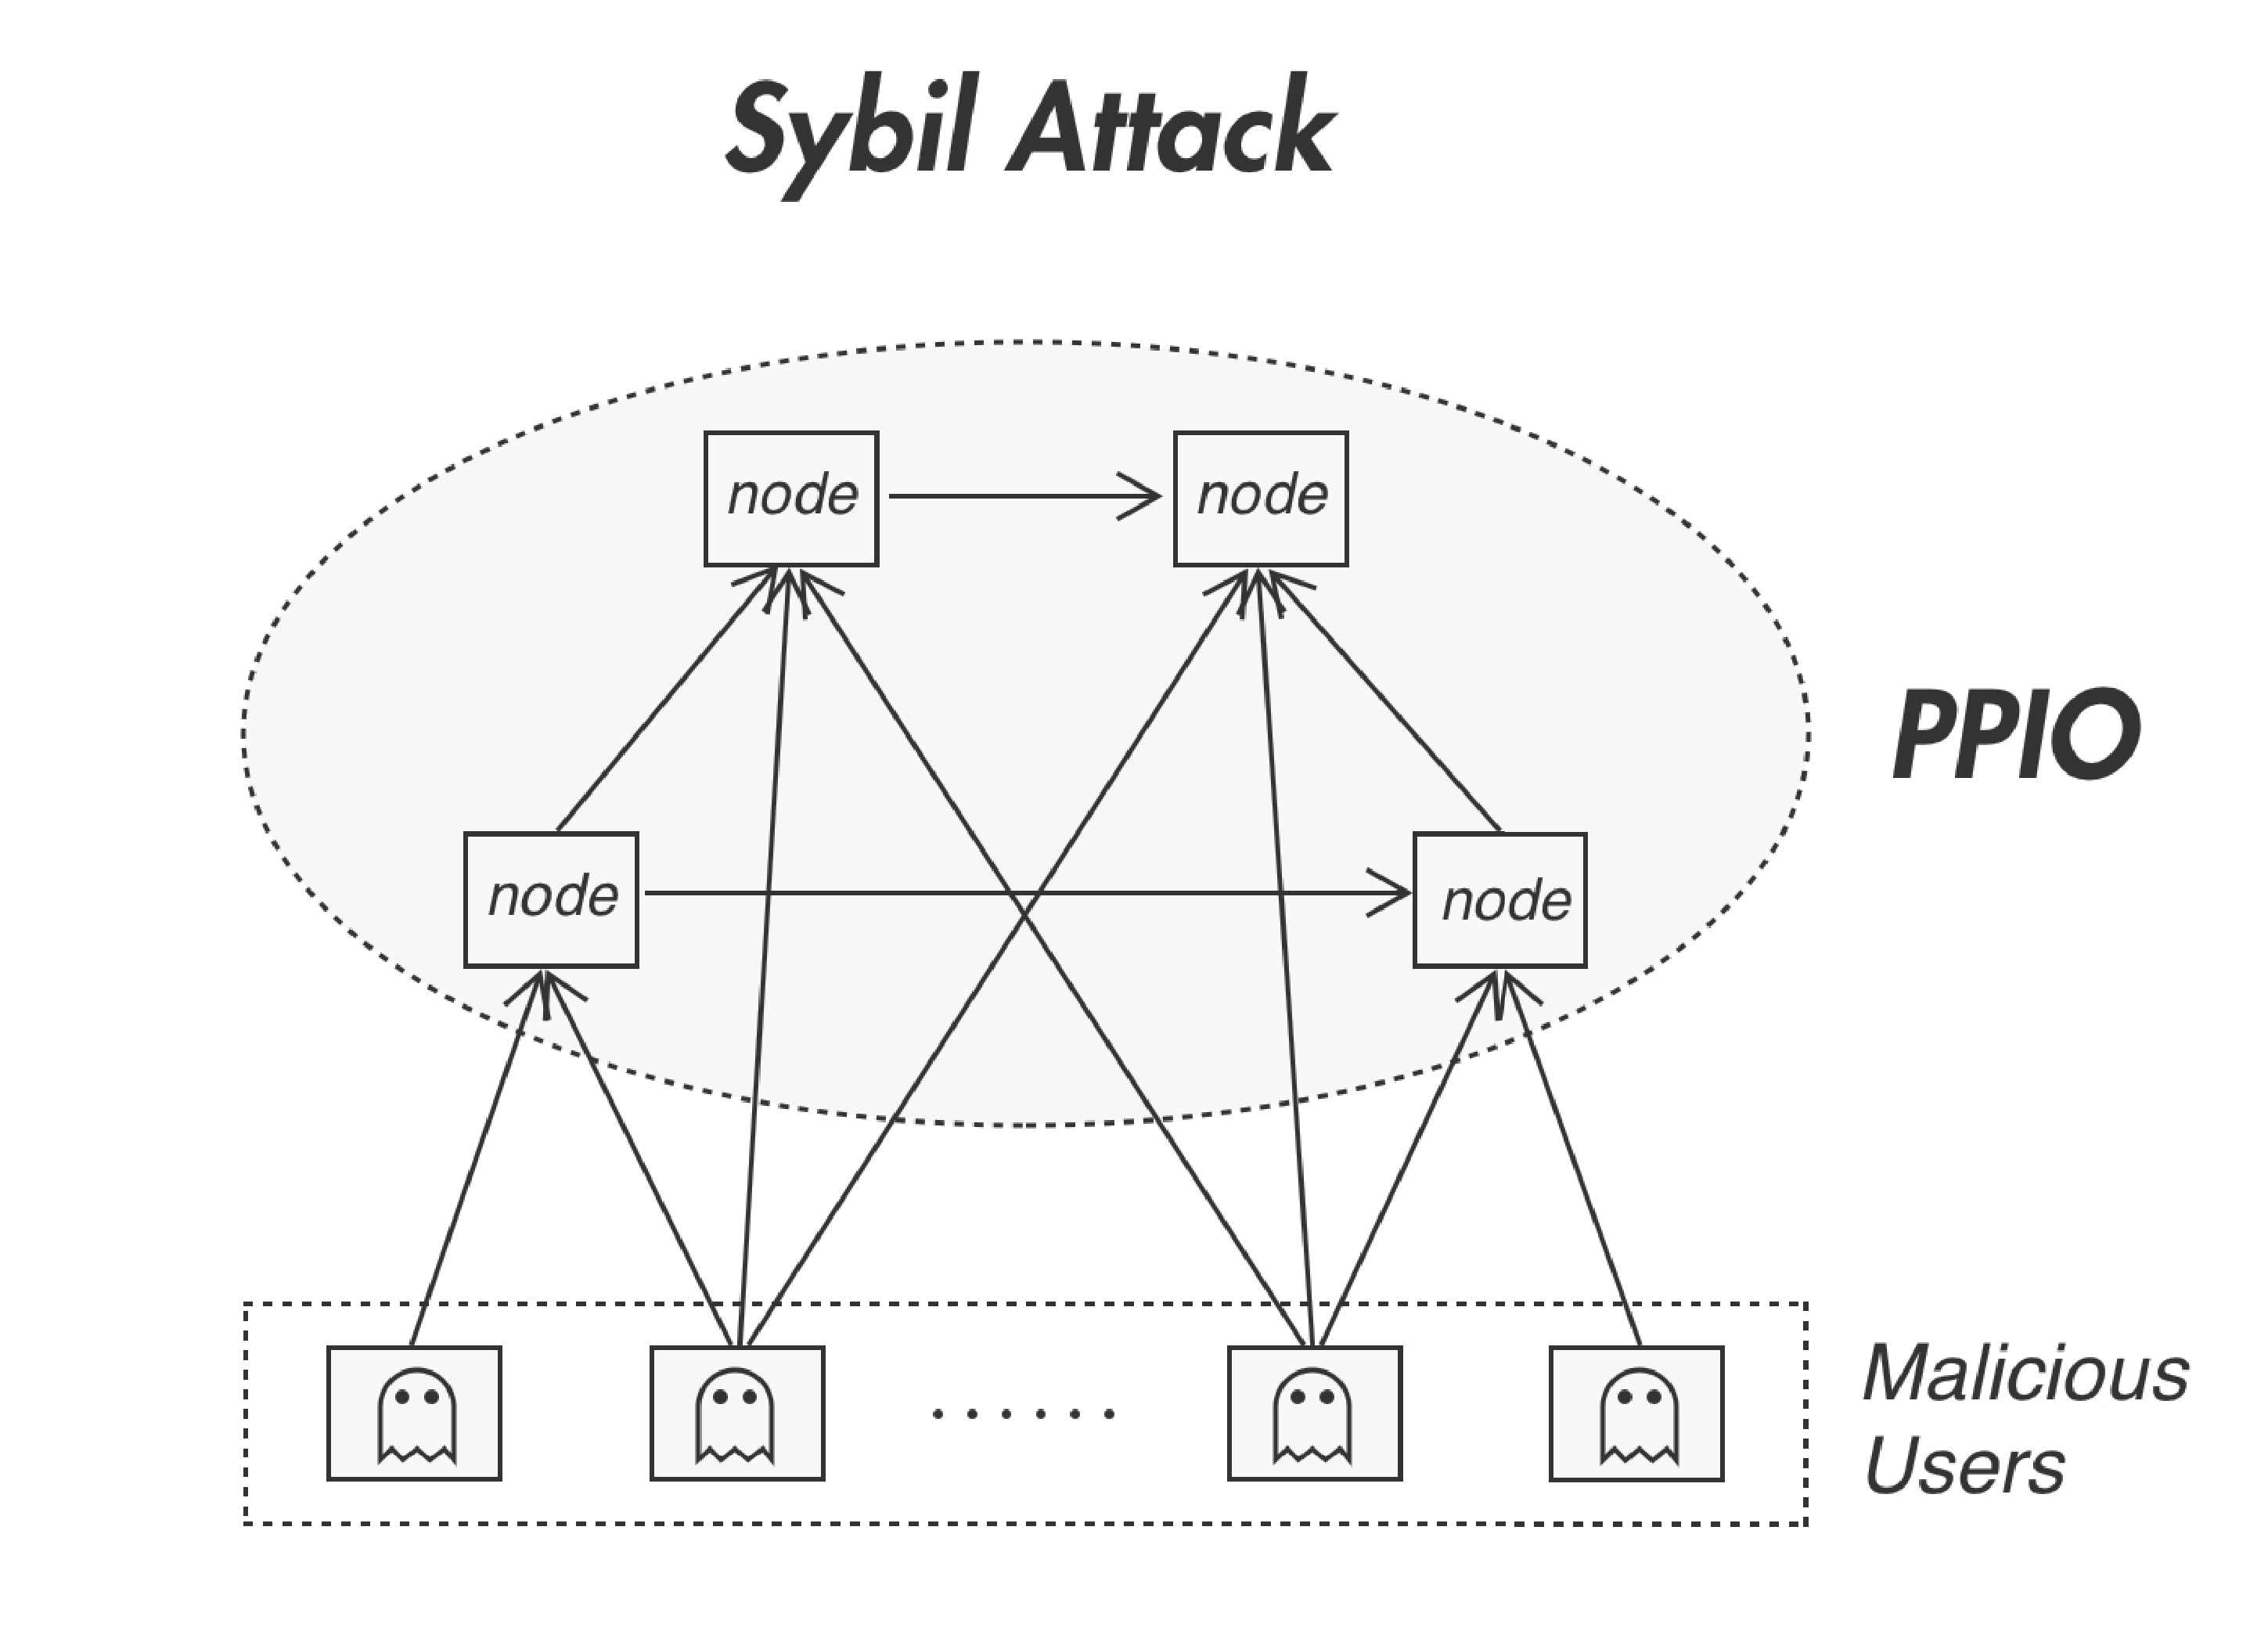
\includegraphics[width=360pt]{fig15}}
\\ \centerline{{Figure 4.1 Sybil Attack}}
   \vspace{-1.5em}
\\

\hangafter 1
\noindent   
PPIO’s Proof of Replication (PoRep) and Proof of Spacetime (PoSt) prevent Sybil attacks by requiring each copy of the data to be unique.  As a result, each miner account is supposed to have stored a different copy. The Verifier In both proofs validates the copy based on its uniquely constructed Merkle tree. As it takes a significant amount of time to recreate a copy to calculate the correct Merkle tree, both proofs will fail or timeout if the miner has not correctly stored its unique copy. 

      \subsection{Outsourcing Attacks}  %——4.2
As shown in Figure 4.2, outsourcing attacks take place when miners claim to have stored copies of the data in their physical storage, but they in fact have stored the data on a third-party storage system. These miners fulfill the download request by forwarding data from the third-party storage to the user. When multiple miners follow suit, the third-party storage system may only store a single copy of the data to save cost, and service it to multiple miners. As a result, the attack reduces the actual data redundancy in the system. Besides, when the third-party storage is a centralized storage system, it increases the risk of data not getting recovered when there is a failure with the centralized server.
   \vspace{-0.5em}
\\
\\ \centerline{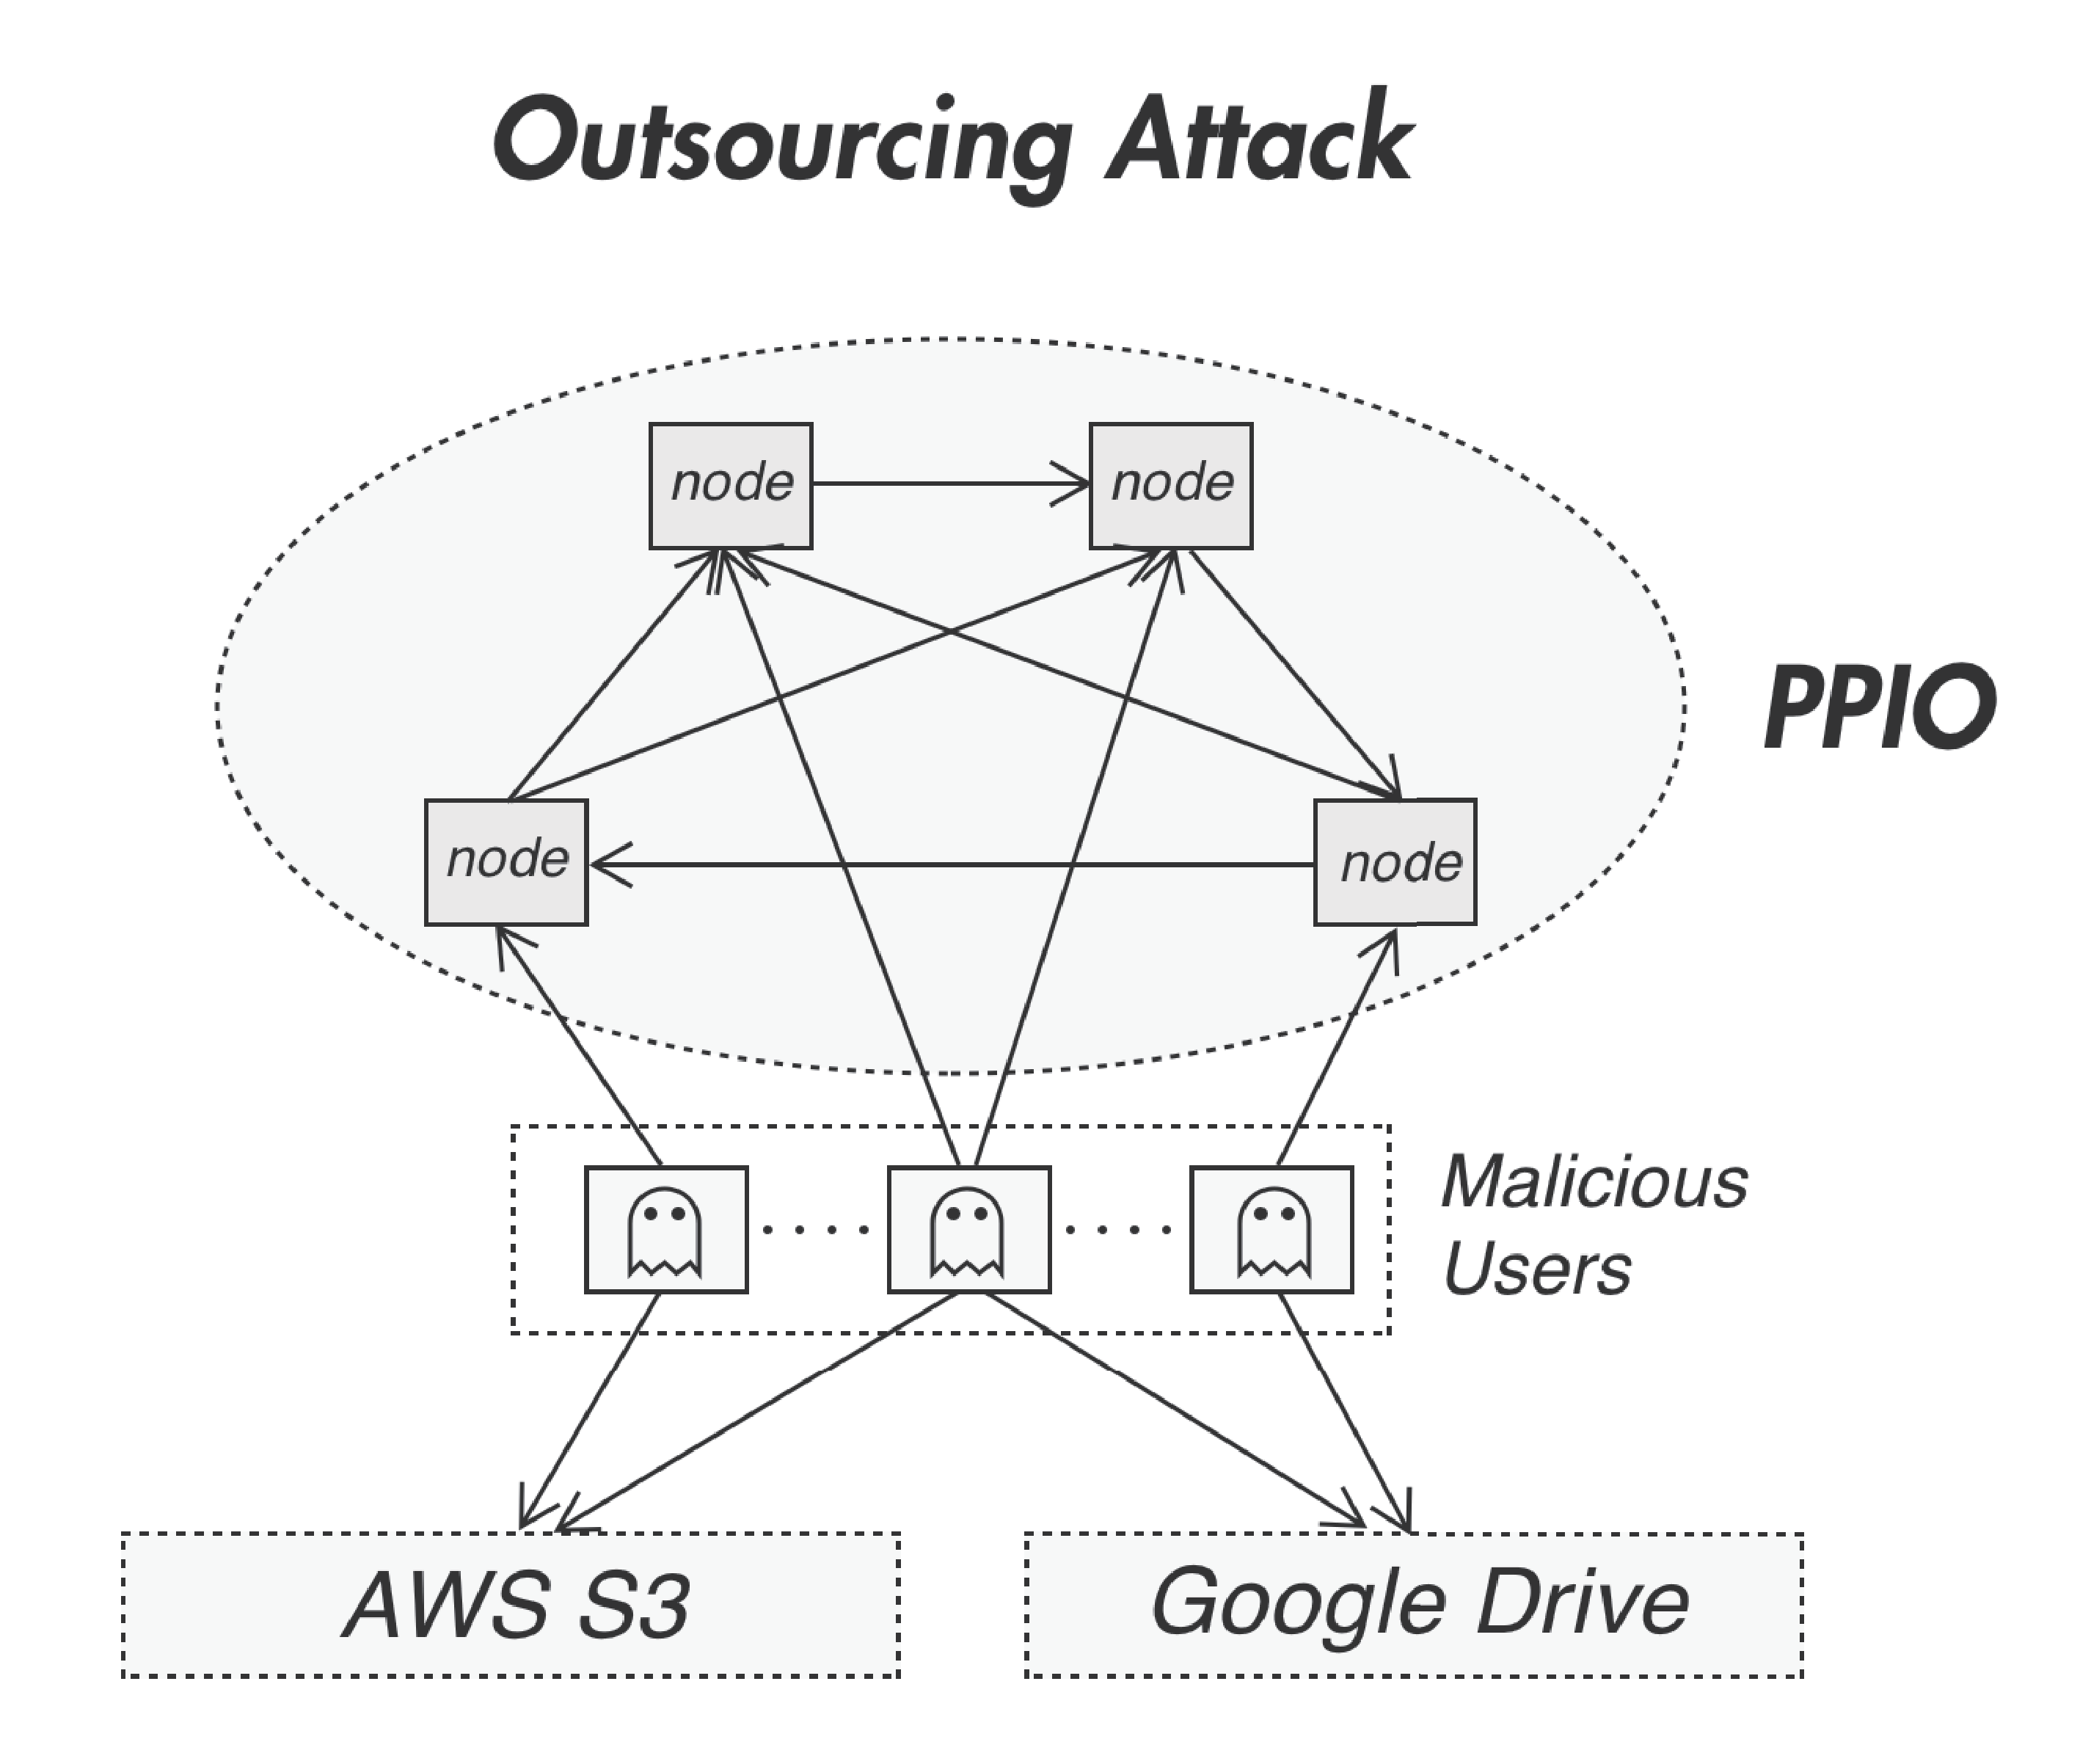
\includegraphics[width=340pt]{fig16}}
\\ \centerline{{ Figure 4.2 Outsourcing Attacks}}
   \vspace{-1.5em}
 \\

\hangafter 1
\noindent   
PPIO’s PoSt can effectively defend against the generation attacks, as the miners need to periodically prove the storage of data assets on their physical storage. The copy of the data each miner stores has to be unique, therefore it significantly increases the difficulty for any miner node to conduct outsourcing attack, and it reduces the risk of loss of data redundancy in the network.
   \vspace{-0.5em}
\\\\At the same time, the Verifier in PoSt requires the challenges to be answered within a specified period. When the miner stores data on third-party storage, it takes additional time to retrieve the data before they can generate the correct proofs. As a result, the challenge is likely to timeout and the miner will be punished for failing to provide proofs in time.
   \vspace{-0.5em}
%————————————————————————————————————————————————
      \subsection{Generation Attacks}  %——4.3
As shown in Figure 4.3, generation attacks take place when a miner pretends to have stored a copy of the data, but in fact, it has only stored enough information that can be used to generate the proofs and respond to the storage challenges from a Verifier in real-time. If successful, the miner can claim to have stored a large amount of data and get unfair rewards. On the other hand, since the user cannot download the correct data from the miner, the reliability of the storage system is significantly degraded.
   \vspace{-2.5em}
\\ \centerline{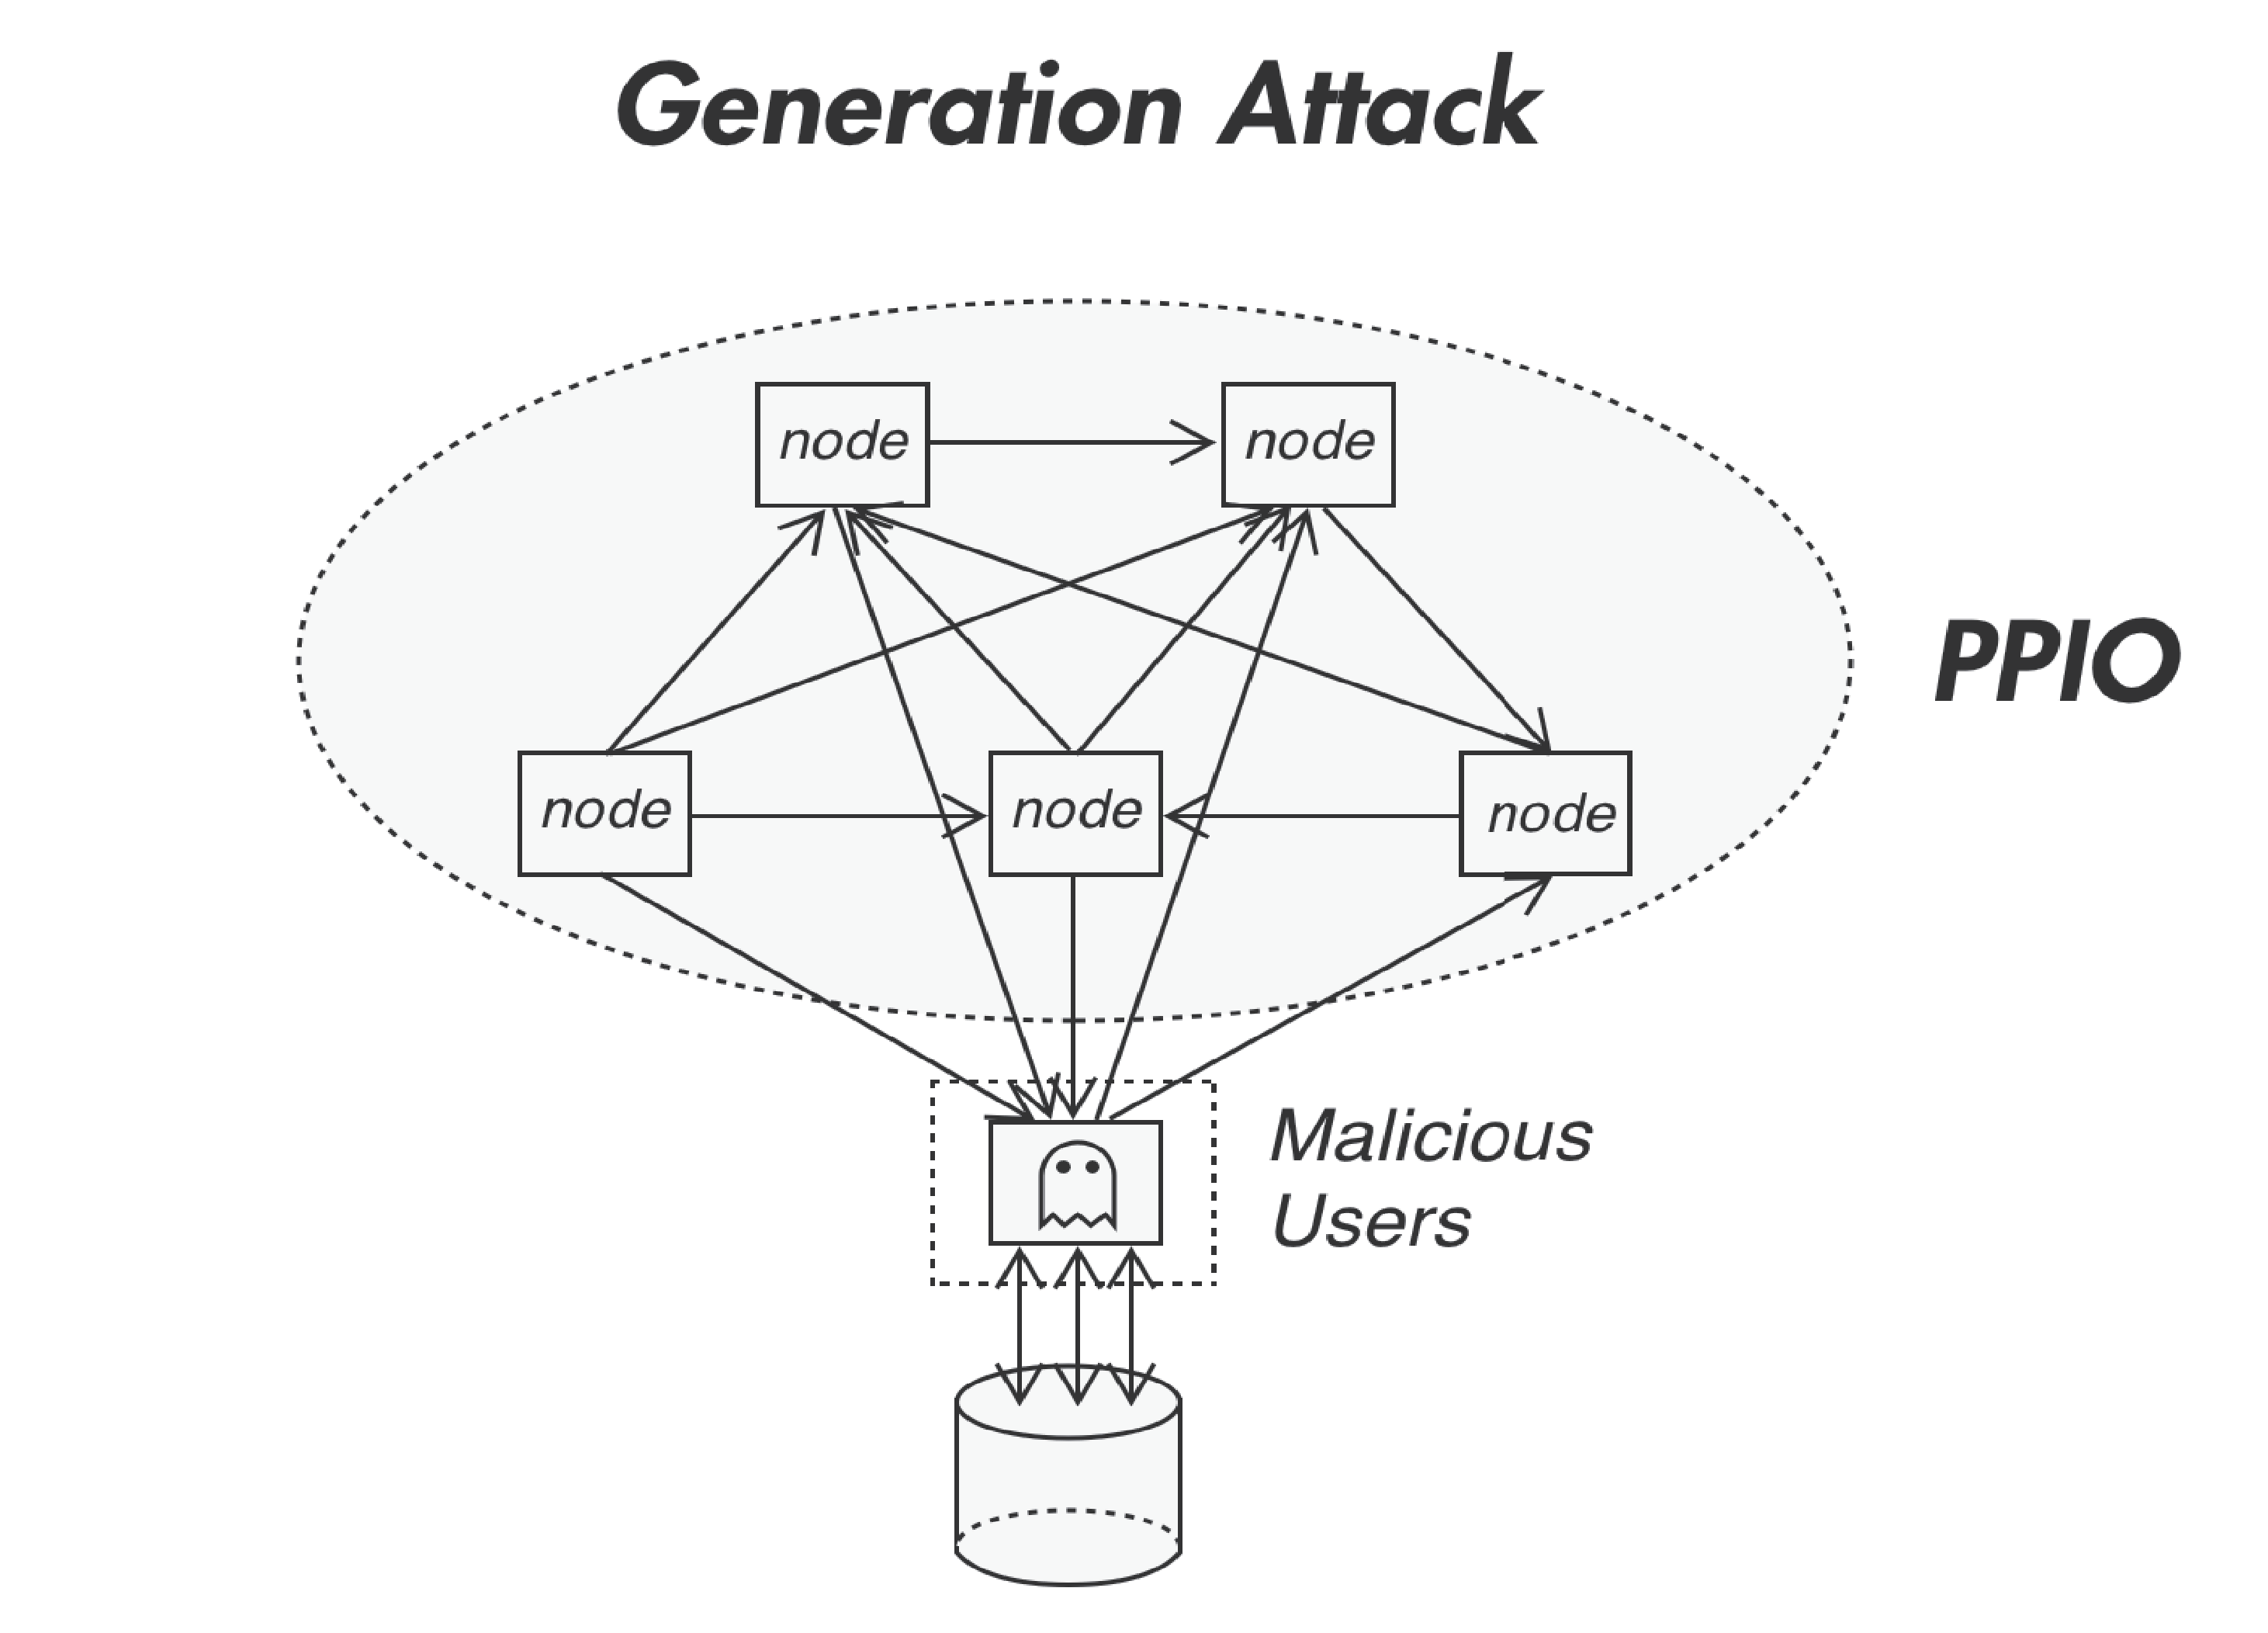
\includegraphics[width=330pt]{fig17}}
\\ \centerline{{Figure 4.3 Generation Attack}}
   \vspace{-1.5em}
\\\\
PPIO can effectively prevent generation attacks with the following design:
   \vspace{-0.8em}
\\

\hangafter 1
\hangindent 1.5em
\noindent   
•\quad PoSt and LPoC require the miners to pre-generate the Merkle tree or DAG from the data, in order satisfy the periodical challenges. It is very time consuming to generate the proofs, and the challenges are likely to time out when the miner attempts the generate them on demand. Even if the miner invests in hardware that enables real-time proof generation, the cost would have outweighed the reward. Therefore miners are not incentivized to conduct generation attacks.
   \vspace{-0.8em}
\\

\hangafter 1
\hangindent 1.5em
\noindent   
•\quad Besides, miners that store the user data also need to provide download service. In PoD, the Verifier validates the data user downloads from the miner. As the miner that conducts generation attacks does not keep an actual copy of the data, PoD will always fail, and the miner will eventually be penalized for not being able to fulfill download requests. This also takes away the incentives for miners to conduct generation attacks.
   \vspace{-0.5em}


      \subsection{Distributed Denial of Service Attacks}  %——4.4
As shown in Figure 4.4, DDoS Attacks take place when a large number of network nodes attack a target node at the same time. For example, the attack can cause a tremendous amount of network traffic that overloads the node, and cause it to fail to respond to regular service requests.
   \vspace{-0.5em}
\\\\
\centerline{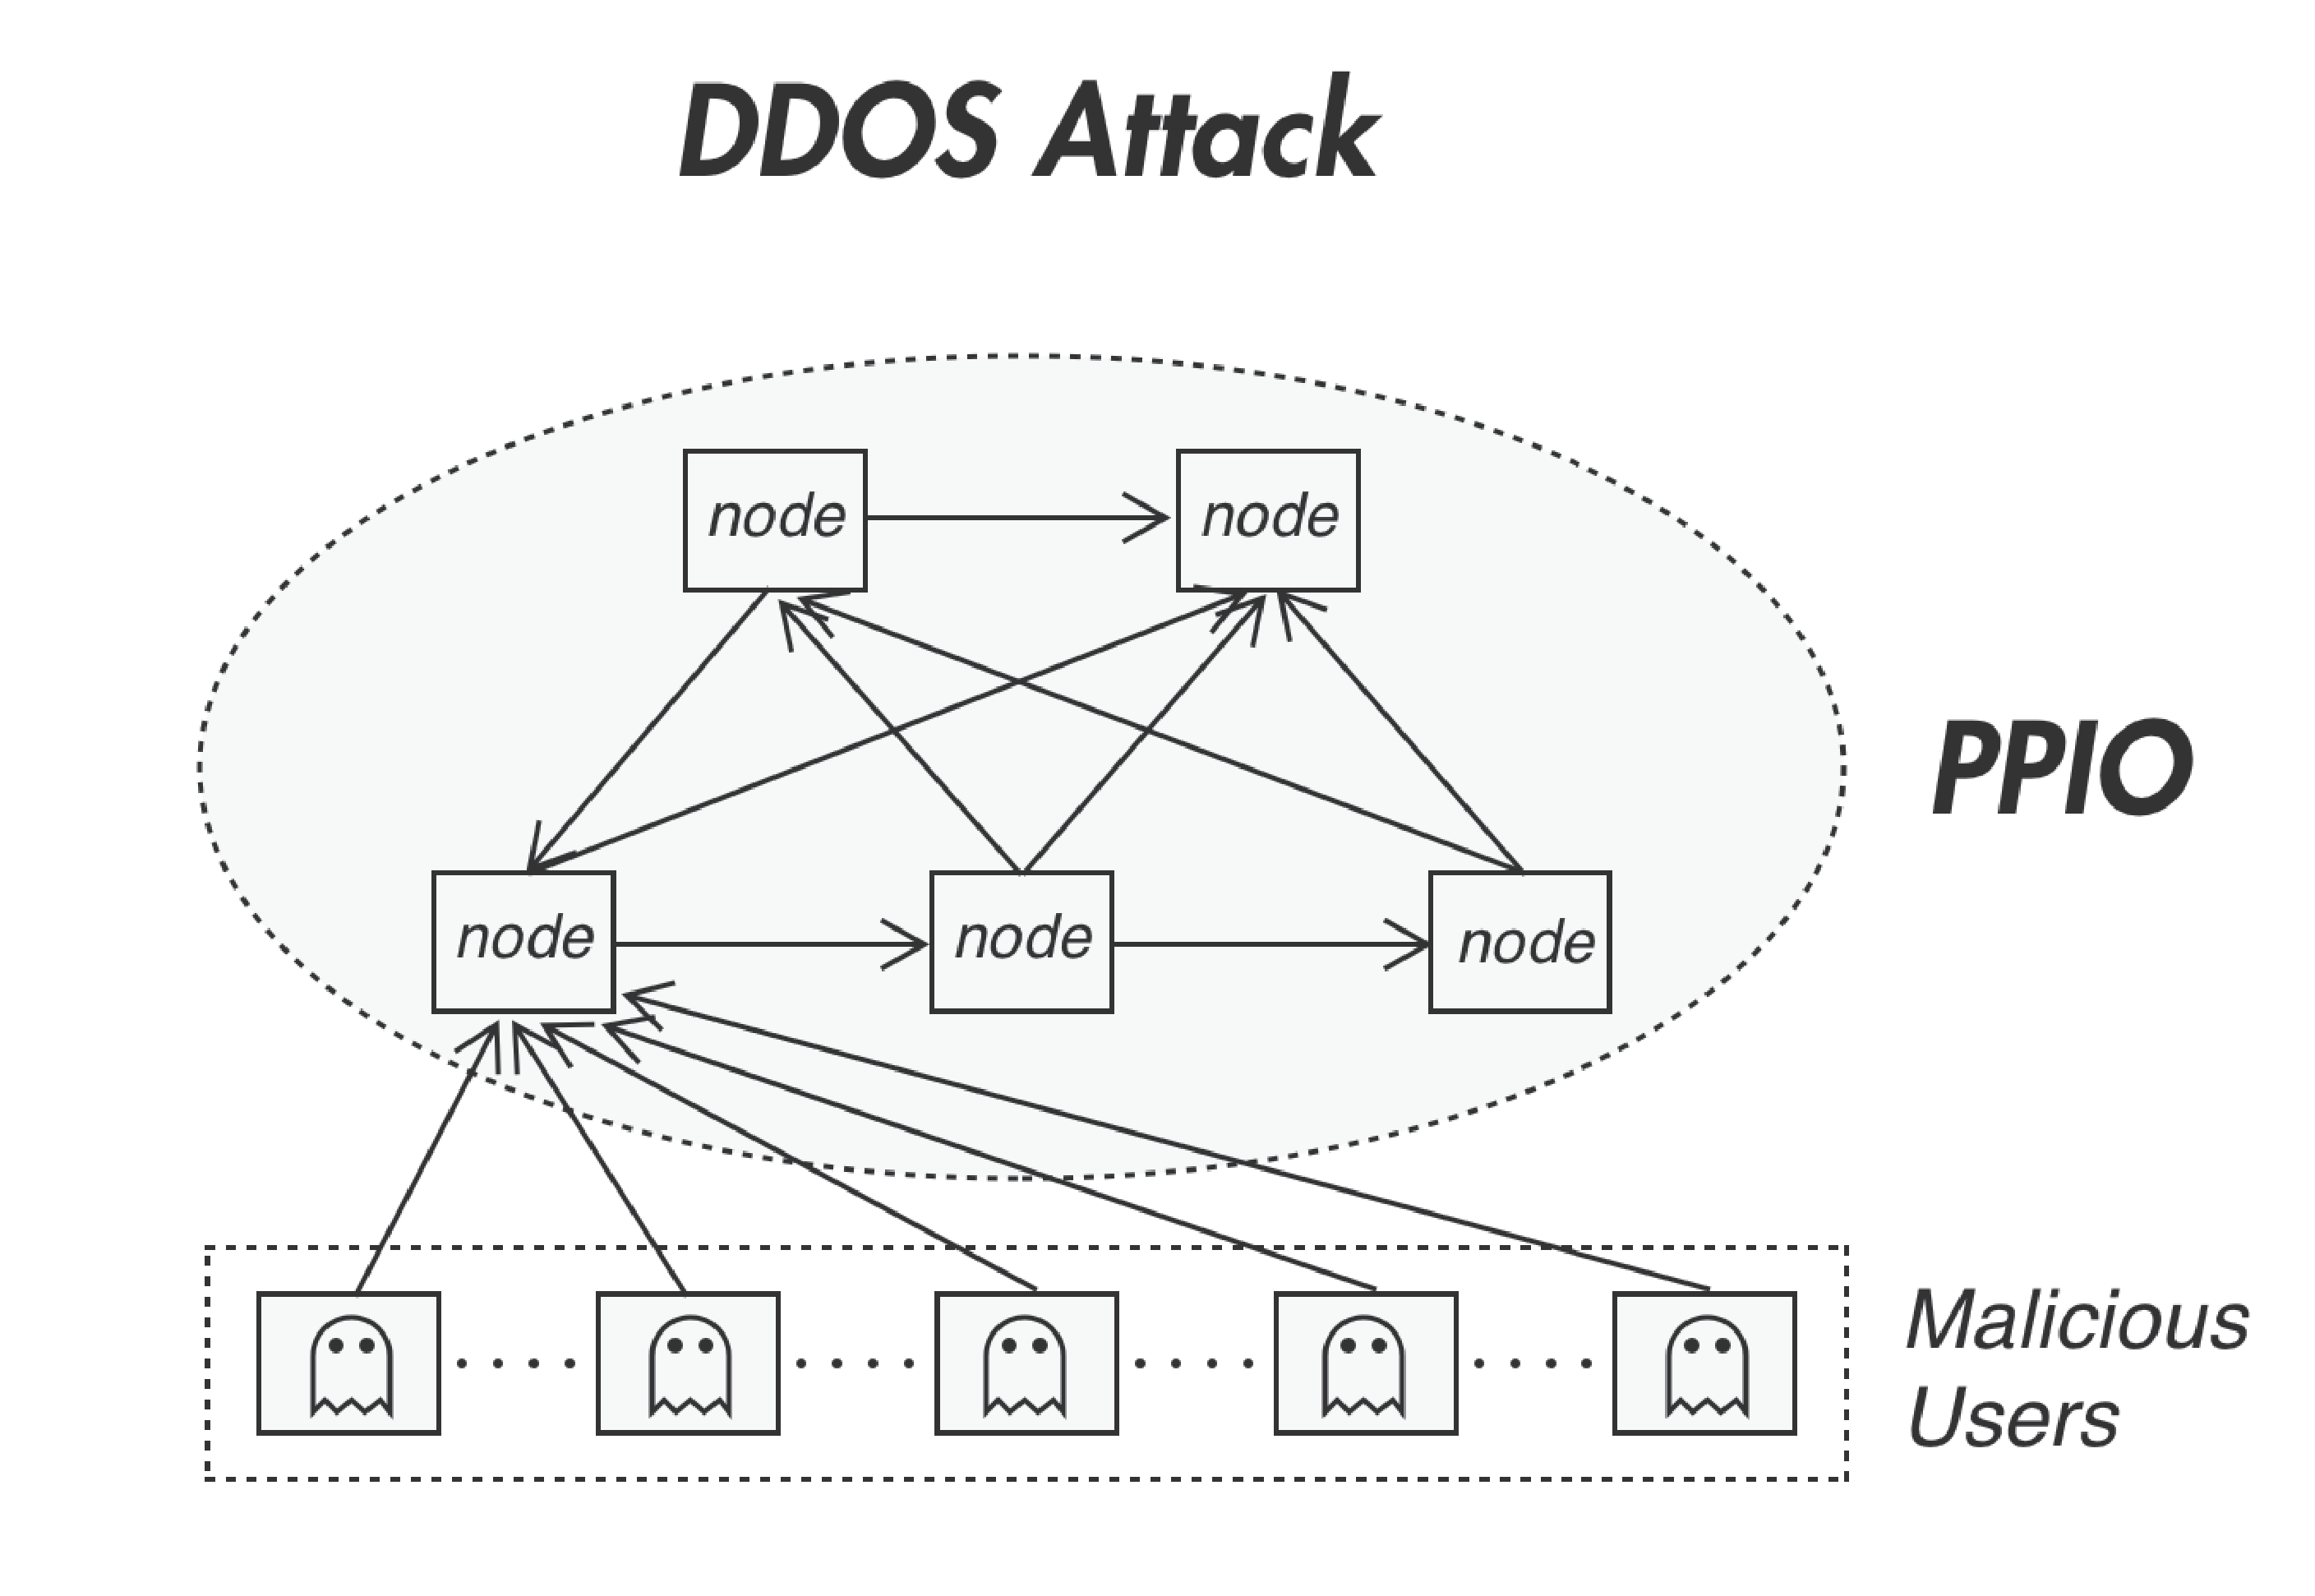
\includegraphics[width=300pt]{fig18}}
 \\ \centerline{{Figure 4.4 DDoS Attacks}}
    \vspace{-1.5em}
\\\\
PPIO can effectively prevent DDoS Attacks with the following design:
   \vspace{-0.8em}
\\

\hangafter 1
\hangindent 1.5em
\noindent   
•\quad For a node to use any service in PPIO, it needs to offer payment (or spend Gas). It will cost the attackers a large sum of money to overload a node.  Therefore it becomes costly to conduct DDoS attack effectively in PPIO’s network.
   \vspace{-0.8em}
\\

\hangafter 1
\hangindent 1.5em
\noindent   
•\quad In PPIO’s consensus mechanism, nodes are being randomly selected to build the next block in the ledger. Unless the attacker attacks all the available nodes in the entire network, the operation of PPIO will not be affected. As a result, it is unrealistic for attackers to conduct effective DDoS attacks against PPIO.
   \vspace{-0.5em}
      \subsection{Eclipse Attacks}  %——4.5
As shown in Figure 4.5, eclipse attacks take place when attackers isolate a victim node by controlling all the connections to and from the node. As a result, the victim node no longer receives correct information from the rest of the network and therefore can be manipulated by the attackers, and may end up with economic losses.
\\
\centerline{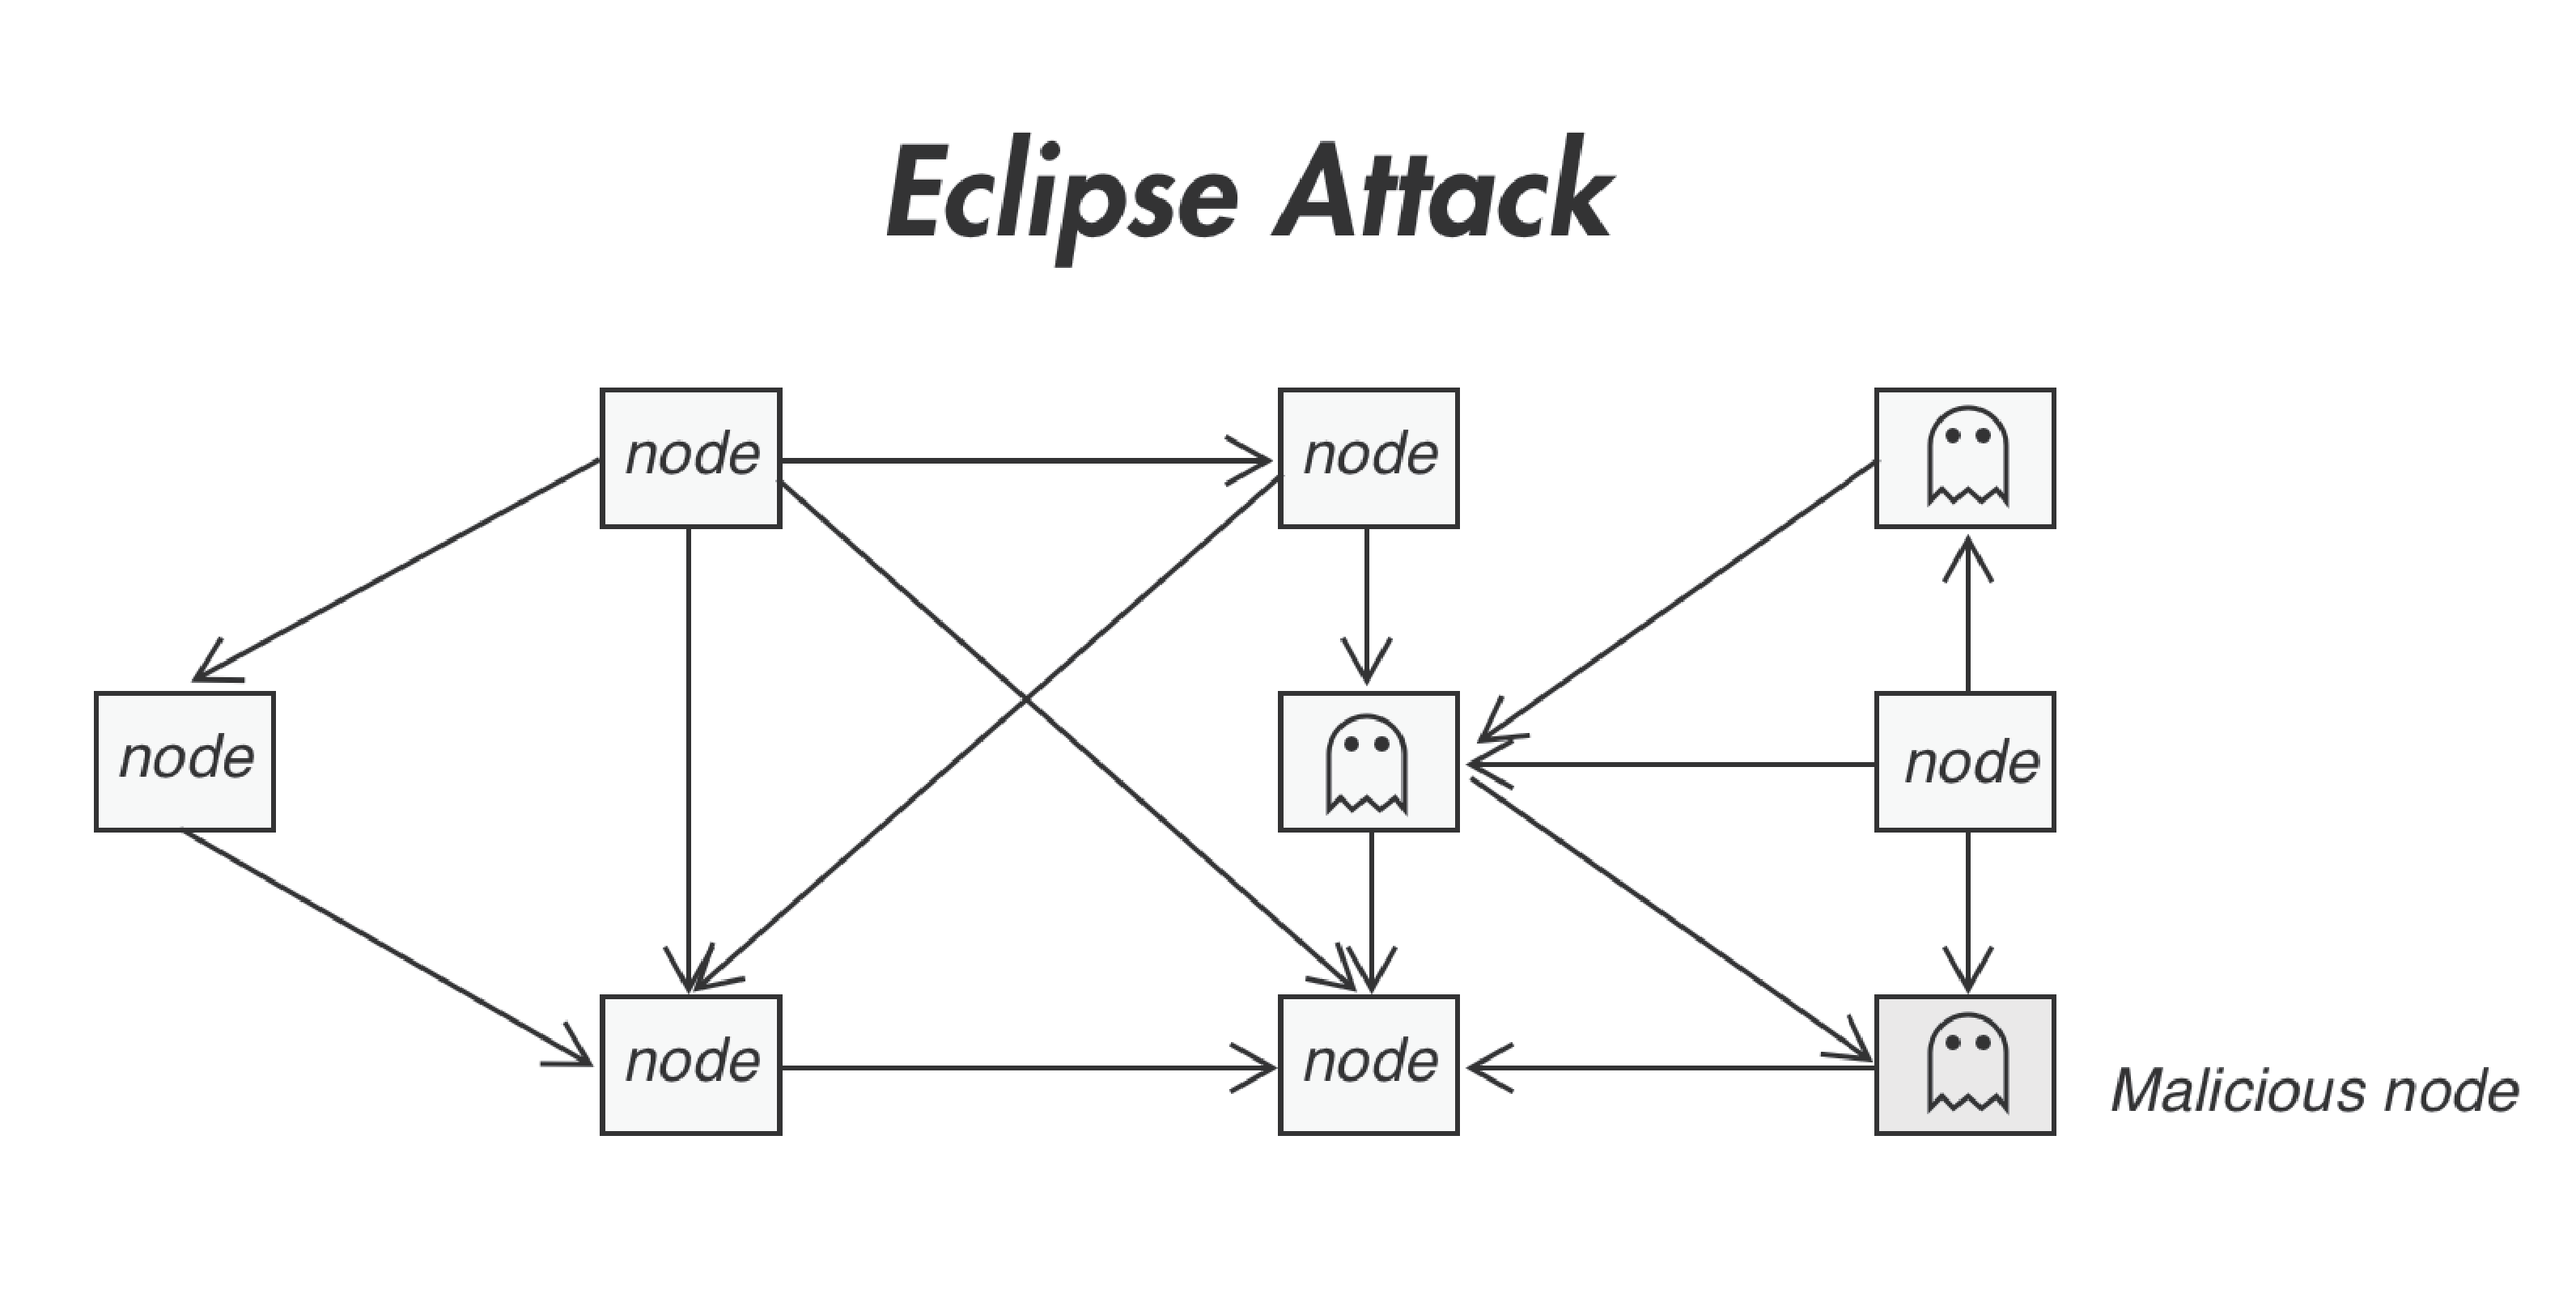
\includegraphics[width=340pt]{fig19}}
 \centerline{{Figure 4.5 Eclipse Attacks }}
    \vspace{-1.5em}
\\ \\PPIO can effectively prevent Eclipse Attacks with the following design:
    \vspace{-0.6em}
\\

\hangafter 1
\hangindent 1.5em
\noindent   
•\quad In PPIO’s blockchain network,  the way that connections are established among different nodes is not purely based on their peer IDs. Constraints on IP addresses are also applied. As a result, the attackers need to own a considerable of IP addresses to isolate target nodes effectively. Therefore it substantially increases the cost of conducting eclipse attacks.
   \vspace{-0.6em}
\\

\hangafter 1
\hangindent 1.5em
\noindent   
•\quad The core functionality in PPIO’s network is distributed among different nodes, that makes it harder to attack. For example, there are multiple Indexer nodes and Verifier nodes in the network. Even if the attackers manage to isolate the Indexer node, the Verifier node is still working and can help discover the attack, and vice versa. Therefore the attackers will have to control the majority of the Indexer nodes and Verifier nodes in the network, making it economically infeasible to conduct effective eclipse attacks.
   \vspace{-0.5em}


   \section{Ecosystem} %——6
Members participating in PPIO’s ecosystem take on different roles, like Users, Miners, Verifiers or Indexers.  The system incentivizes each member for assuming their responsibility. They are rewarded for performing their functionalities and making a contribution to the network. They are penalized for failing to fulfill their responsibility or conducting illegal operations. As the network operates in an open and fair environment, it encourages members to contribute more resources to the network, attracts new members to participate and help maintain a healthy and sustaining ecosystem.
   \vspace{-0.5em}
\\\\\ PPIO’s design also employs some mechanisms that help stabilize its economy. The Cryptocurrency used in PPIO’s system to collect rewards or purchase services is called PPIO Coin. PPIO offers a price lock program that allows the user to take advantage of lower prices when the cost of storage and bandwidth drops. At the same time, it protects the user from price hikes when the resource cost rises due to inevitable market fluctuation.  PPIO employs an Oracle system to guide the pricing of storage and download services, that helps reduce the volatility of PPIO Coin so that users and developers can enjoy a more stable economy. PPIO also employs a payment mechanism called Coin-Pool, that allows users to purchase storage services in bulk. It helps make the payment system more flexible and easy-to-use.
   \vspace{-0.5em}
   
      \subsection{Roles} %——5.1
The following roles exist in PPIO’s storage system:
   \vspace{-0.8em}
\\

\hangafter 1
\hangindent 1.5em
\noindent   
•\quad {\bf User Node} 
   \vspace{-0.8em}
\\ \\Users are the consumers of the PPIO storage system, and they acquire storage and download services by consuming certain amount of PPIO Coin.
   \vspace{-0.8em}
\\

\hangafter 1
\hangindent 1.5em
\noindent   
•\quad {\bf Source Node}
   \vspace{-0.8em}
\\ \\In the PCDN use scenario, the source node is a special user node that publishes content, it usually stays online and provides download services to other users.
   \vspace{-0.8em}
\\

\hangafter 1
\hangindent 1.5em
\noindent   
•\quad {\bf Miner Node}
   \vspace{-0.8em}
\\ \\The node that provides storage and bandwidth resource in PPIO’s network, and receives PPIO Coins for its contribution.
   \vspace{-0.6em}
\\

\hangafter 1
\hangindent 1.5em
\noindent   
•\quad {\bf Indexer Node}
   \vspace{-0.8em}
\\ \\The nodes that provide both indexing and scheduling services to the network, and receive PPIO Coin rewards accordingly. Their indexing service helps the user quickly locate stored data. Their scheduling service manages data storage and download, and it also facilitates content delivery by adjusting how the copies of data are distributed in the network.
   \vspace{-0.8em}
\\

\hangafter 1
\hangindent 1.5em
\noindent   
•\quad {\bf Verifier Node}
   \vspace{-0.8em}
\\ \\The nodes that conduct and validate storage proofs in the network, and receive rewards accordingly. They are responsible for verifying the available storage capacity of miners, confirming data storage and download, validating storage spacetime and effective bandwidth.
   \vspace{-0.6em}
\\

\hangafter 1
\hangindent 1.5em
\noindent   
•\quad {\bf CoinPool Node}
   \vspace{-0.5em}
\\ \\The nodes that provide payment services to the users, with more friendly payment options for the storage.
\\

\noindent   
Any of the above nodes can also participate in PPIO’s consensus mechanism by choice and becomes eligible to build new blocks on the ledger. With PPIO’s PVFT consensus algorithm, the participating nodes compete to become next block builder in a fair fashion. When a node is selected and successfully builds the next block, it also gets rewarded accordingly.
   \vspace{-0.5em}
      \subsection{Mining}  %——5.2
In PPIO’s storage network, miners get rewarded by providing storage or download services. Besides, they also get a chance to receive mining rewards from the platform, when new blocks are generated on the distributed ledger.
   \vspace{-0.5em}
\\ \\PPIO’s mining reward is distributed based on the contribution of each miner, measured with storage proofs. The purpose of the reward is to encourage miners to participate, contribute more resource and provide better service to the network. PPIO allows miners to collect mining rewards in two ways, non-collateralized collection, and collateralized collection.
   \vspace{-0.8em}
\\

\hangafter 1
\hangindent 1.5em
\noindent   
•\quad {\bf Non-collateralized mining}: The miners are allowed to collect mining rewards without having enough PPIO Coins as collateral. However, the rewards distributed to the miner will be deposited as collateral and cannot be withdrawn by the miner, until a minimal amount of deposit is reached. This method is mainly designed for newly joined miners. It allows them to start building the necessary deposit and credit while providing service to the network. After the minimal amount of deposit for the services collateral is reached and maintained, the miner will start collateralized mining reward collection.
   \vspace{-0.8em}
\\

\hangafter 1
\hangindent 1.5em
\noindent   
•\quad {\bf Collateralized mining}: The miner's deposit PPIO Coins as collateral and commitment to the services they provide. When miners do not fulfill the services they promised, not only will they become ineligible to receive more mining rewards, they will also lose part of the deposit as a punishment. The amount of required deposit is proportional to the length of service they sign up to provide, the longer the service term is, the higher the deposit will be.
   \vspace{-0.5em}
\\

\noindent  
PPIO’s mining rewards are distributed by weighing the contribution of the miners. Each miner ‘s weight $W$ is decided by its accumulated storage proofs, calculated with the following formula:
$$
W=(\alpha f(PoRep) + \beta f(PoSt) + \gamma f(PoMD) + \sigma f(PoLC) )\cdot\delta
$$
where $\delta$ is the collateral parameter. Assuming two miners have an equal accumulated contribution, the
miner with a longer future service commitment will be assigned a higher collateral parameter, and thus receives higher mining rewards.
   \vspace{-0.5em}
\\\\
The default values of the scaling factors of each proof are as follows:\\
   \vspace{-0.5em}
 \begin{center}
\begin{tabular}{|p{2.7cm}<{\centering}|p{3.4cm}<{\centering}|p{3cm}<{\centering}|}% 通过添加 | 来表示是否需要绘制竖线
\hline  % 在表格最上方绘制横线
 Parameters & Description & Default Value \\
\hline  %在第一行和第二行之间绘制横线
 $\alpha$& PoRep Scaling Factor&20\% \\
 \hline  %在第一行和第二行之间绘制横线
 $\beta$&PoSt Scaling Factor&40\%\\
 \hline  %在第一行和第二行之间绘制横线
  $\gamma$&PoD Scaling Factor&30\% \\
 \hline  %在第一行和第二行之间绘制横线
  $\sigma$&LPoC Scaling Factor&10\%\\

\hline % 在表格最下方绘制横线
\end{tabular}
\end{center} 
 \vspace{0.5em}
During the early stage deployment of PPIO, it is expected that the amount of stored data and storage transactions will start low. For encouraging new miners to join the network and make their storage capacity available, the scaling factor of LPoC will be raised in this period. As the storage volume grows, the scaling factor of LPoC will be gradually reduced, while the scaling factors of the other storage proofs will be increased.
 \vspace{-0.5em}
\\ \\When a new block is added to PPIO’s distributed ledger, a certain amount of PPIO Coins is created as a reward. However, the node that builds the block does not receive all the reward. Instead, most of the reward is distributed to the miners, based on the calculated weight of each miner from their storage and bandwidth contribution during the time period.\\\\
The PPIO Coins created for new blocks are distributed as follows:\\
 \vspace{-0.5em}
 \begin{center}
\begin{tabular}{|p{4cm}<{\centering}|p{4cm}<{\centering}|}% 通过添加 | 来表示是否需要绘制竖线
\hline  % 在表格最上方绘制横线
Role&Percentage of Distribution \\
 \hline  % 在表格最上方绘制横线
Block Producer &5\% \\
 \hline  %在第一行和第二行之间绘制横线
 Miners&90\%\\
 \hline  %在第一行和第二行之间绘制横线
   Verifiers&4\% \\
 \hline  %在第一行和第二行之间绘制横线
Indexers &1\%\\

\hline % 在表格最下方绘制横线
\end{tabular}
\end{center} 
      \subsection{Smart Contract}  %——5.3
Self-executing smart contracts are used in PPIO storage network to handle data storage or download.
 \vspace{-0.8em}
%\\ \\However, Lessors may go offline at any moment in time over the heterogeneous nature of P2P network, and new Lessors are required to fulfill the storage needs for these Segments. The purpose of this event handling is to ensure sufficient copies of Segments at all times.
%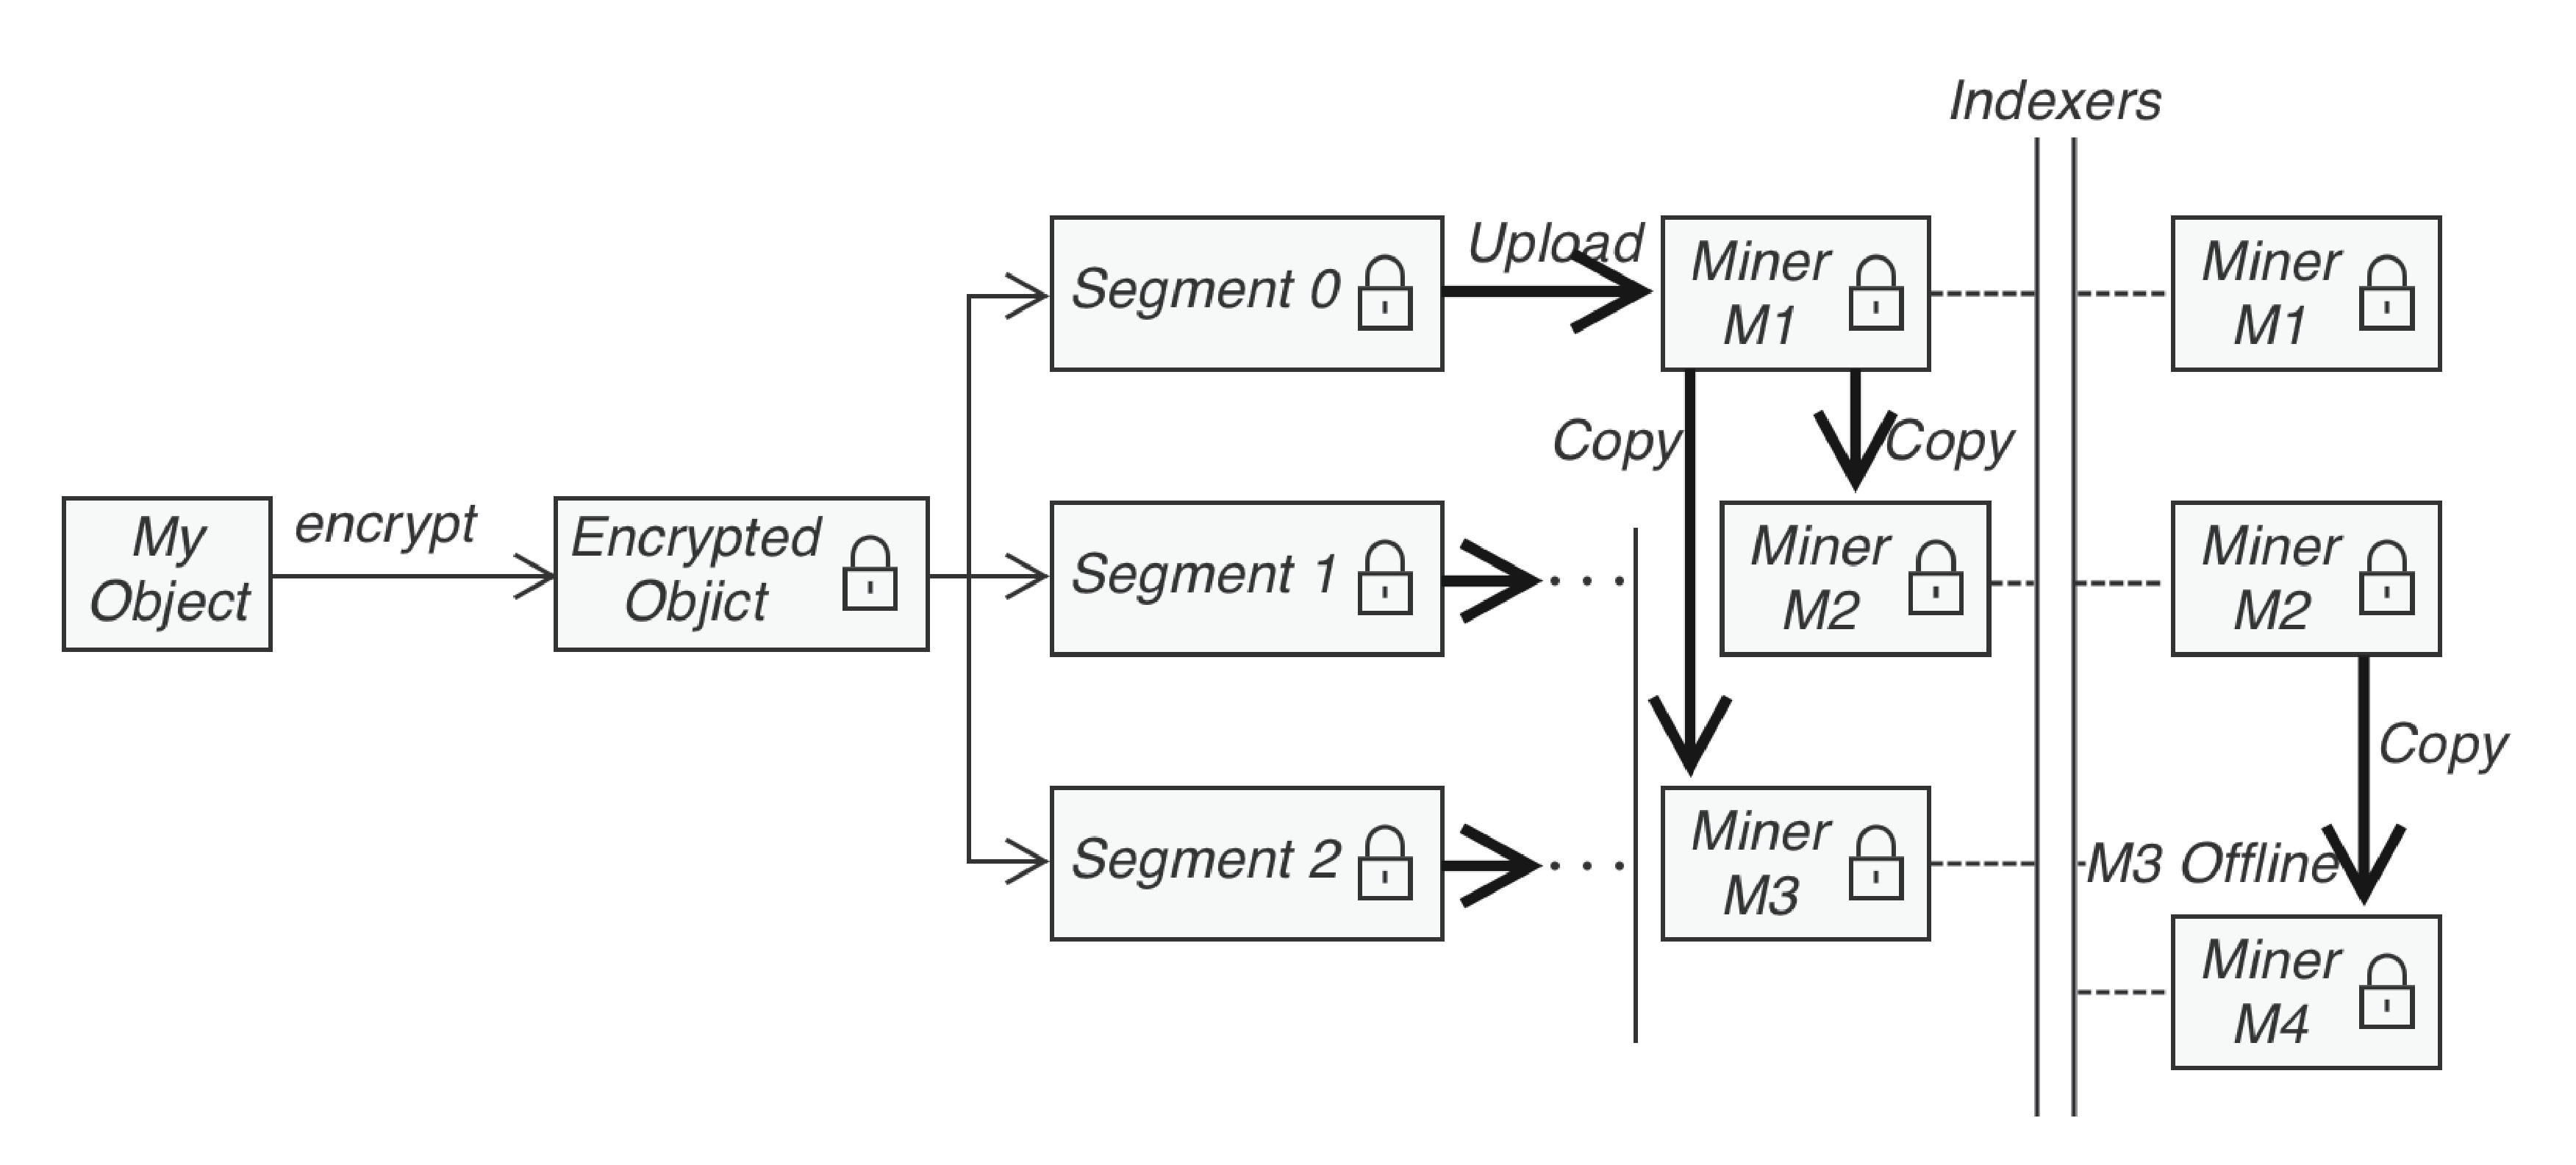
\includegraphics[width=450pt]{fig20}
%\\ \centerline{\large{fig: eclipse attack}}%——————————————————————————————待确认名称 
 %PPIO applies self-executing smart contracts in both of our download and upload procedures, primarily taking the form of a Storage Contract or a Download Contract.
\\

\hangafter 1
\hangindent 1.5em
\noindent   
•\quad {\bf Storage Contract:} 
The contract is created when the user stores an object onto the PPIO storage network. It specifies the storage period and the number of PPIO Coins to be paid for the storage service. Once the contract is executed, the object will be stored during the specified period with the agreed price, regardless of price fluctuations of PPIO Coin during the period.
 \vspace{-0.8em}
\\

\hangafter 1
\hangindent 1.5em
\noindent   
•\quad {\bf Download Contract:}
The contract is created when the user wants to download a data object from the PPIO storage network. It specifies the number of PPIO Coins to be paid for the service. Once the contract is executed, the miners must provide service immediately for the user to download the data.
 \vspace{-0.6em}
\\

\noindent   
An executed storage contract can be updated by:
 \vspace{-0.8em}
\\

\hangafter 1
\hangindent 1.5em
\noindent   
•\quad {\bf Storage Renewal:} 
A Storage Contract can be renewed to extend the storage period. For example, the maximal storage period of any new contract in PPIO is 365 days. But an extension can be made by renewing the contract before the expiration date.
 \vspace{-0.8em}
\\

\hangafter 1
\hangindent 1.5em
\noindent   
•\quad {\bf Storage Termination:}
PPIO allows the user to terminate a storage contract before the expiration date. The user will get refunded the number of PPIO Coins that have yet to be spent in the contract.
 \vspace{-0.8em}
\\

\hangafter 1
\hangindent 1.5em
\noindent   
•\quad {\bf Storage Update:}
PPIO allows the user to update the stored object. A new contract for the updated object will be created and executed, with new payment paid in PPIO Coins. The old contract is terminated, and the remaining PPIO Coins in the contract are returned to the user.
 \vspace{-0.5em}


      \subsection{Gas}  %——5.4
As shown in Figure 5.1 and 5.2, while executing either type of smart contract, PPIO dispatches the miners and other nodes to provide services and rewards them accordingly. PPIO adopts Gas as a unit to quantify the contribution of each node in fulfilling a specific contract. In the end, each node will receive PPIO Coins at an amount based on the number of Gas units. The amount of PPIO Coins the user pays per Gas unit in this contract is called Gas Price.
 \vspace{-0.6em}
\\ \\Gas transactions among different nodes while executing the storage and download contracts are described below.
 \vspace{-0.5em}
\\\\{\bf Storage Contract} 
 \vspace{-0.8em}
\\

\hangafter 1
\hangindent 1.5em
\noindent   
•\quad The User pays Gas for storing each object, in the amount of $G_{u}$.
 \vspace{-0.6em}
\\

\hangafter 1
\hangindent 1.5em
\noindent   
•\quad The Verifier receives Gas for conducting Proof of Space-Time (PoSt), in the amount of $G_{post}$.
 \vspace{-0.6em}
\\

\hangafter 1
\hangindent 1.5em
\noindent   
•\quad The miner receives Gas for providing storage space-time during the storage period, in the amount of $G_{st}$.
 \vspace{-0.5em}
\\

\noindent   
The transactions can be formulated as:
 \vspace{-0.6em}
\\\\
\centerline{$G_{u} = \sum G_{st} + \sum G_{post}$}\\
\centerline{$\sum G_{st}=N_{Copy} \cdot G_{st} $}\\
\centerline{$\sum G_{post}=N_{Verifier}\cdot G_{post}$}
 \vspace{-1.5em}
\\\\Where $N_{Copy}$ is the number of copies stored, and $N_{Verifier}$ is the number of verifiers involved.
 \vspace{-0.6em}
\\\\When storage operation takes place, the miner needs to make Gas payments $G_{l}$ to obtain a copy of the data. The miner does so as it can receive more payments in the future for storing the data and provide download services during the storage period. $G_{rep}$ is the amount of Gas the miner pays to another miner to obtain a copy of the data object. $G_{porep} = N_{Verifier} \cdot G_{porep}$, which is the amount of Gas miner pays to the Verifier for conducting Proof of Replication (PoRep). $G_{schedule}$ is the amount of Gas the miner pays to the Indexer for scheduling the data copy. The total amount the miner pays is $G_{l} = G_{rep} + G_{porep} + G_{schedule}$
%\centerline{$G_{total} = Copies \cdot (G_{st} + G_{post} \cdot N_{Verifieies})$}
%\begin{itemize}
%\item $G_{total}$ %——完全是由上传者支付的;
%\item  $G_{st}$  %——是租户存储文件获得的收入 %
%\item$G_{post}$ %—— 是监督节点获得提供存储证明收入;
%\end{itemize}
%———————————但是整个过程中, 租户既然要获取任务,下载获得未来的时空收益和多点上传收益,那么租户要支付3笔费用:
%\begin{itemize}
%\item $G_{rep}$ %——下载节点支付给上传节点的费用;
%\item  $G_{porep} = N_{Verifier} \cdot g_{porep}$  %——监督节点做复制证明的费用;
%\item $G_{schedule} = g_{schedule}$ %—— 检索调度节点获得调度费用;
%\end{itemize}
%——————存储合约的执行网络架构图
\\\\ \centerline{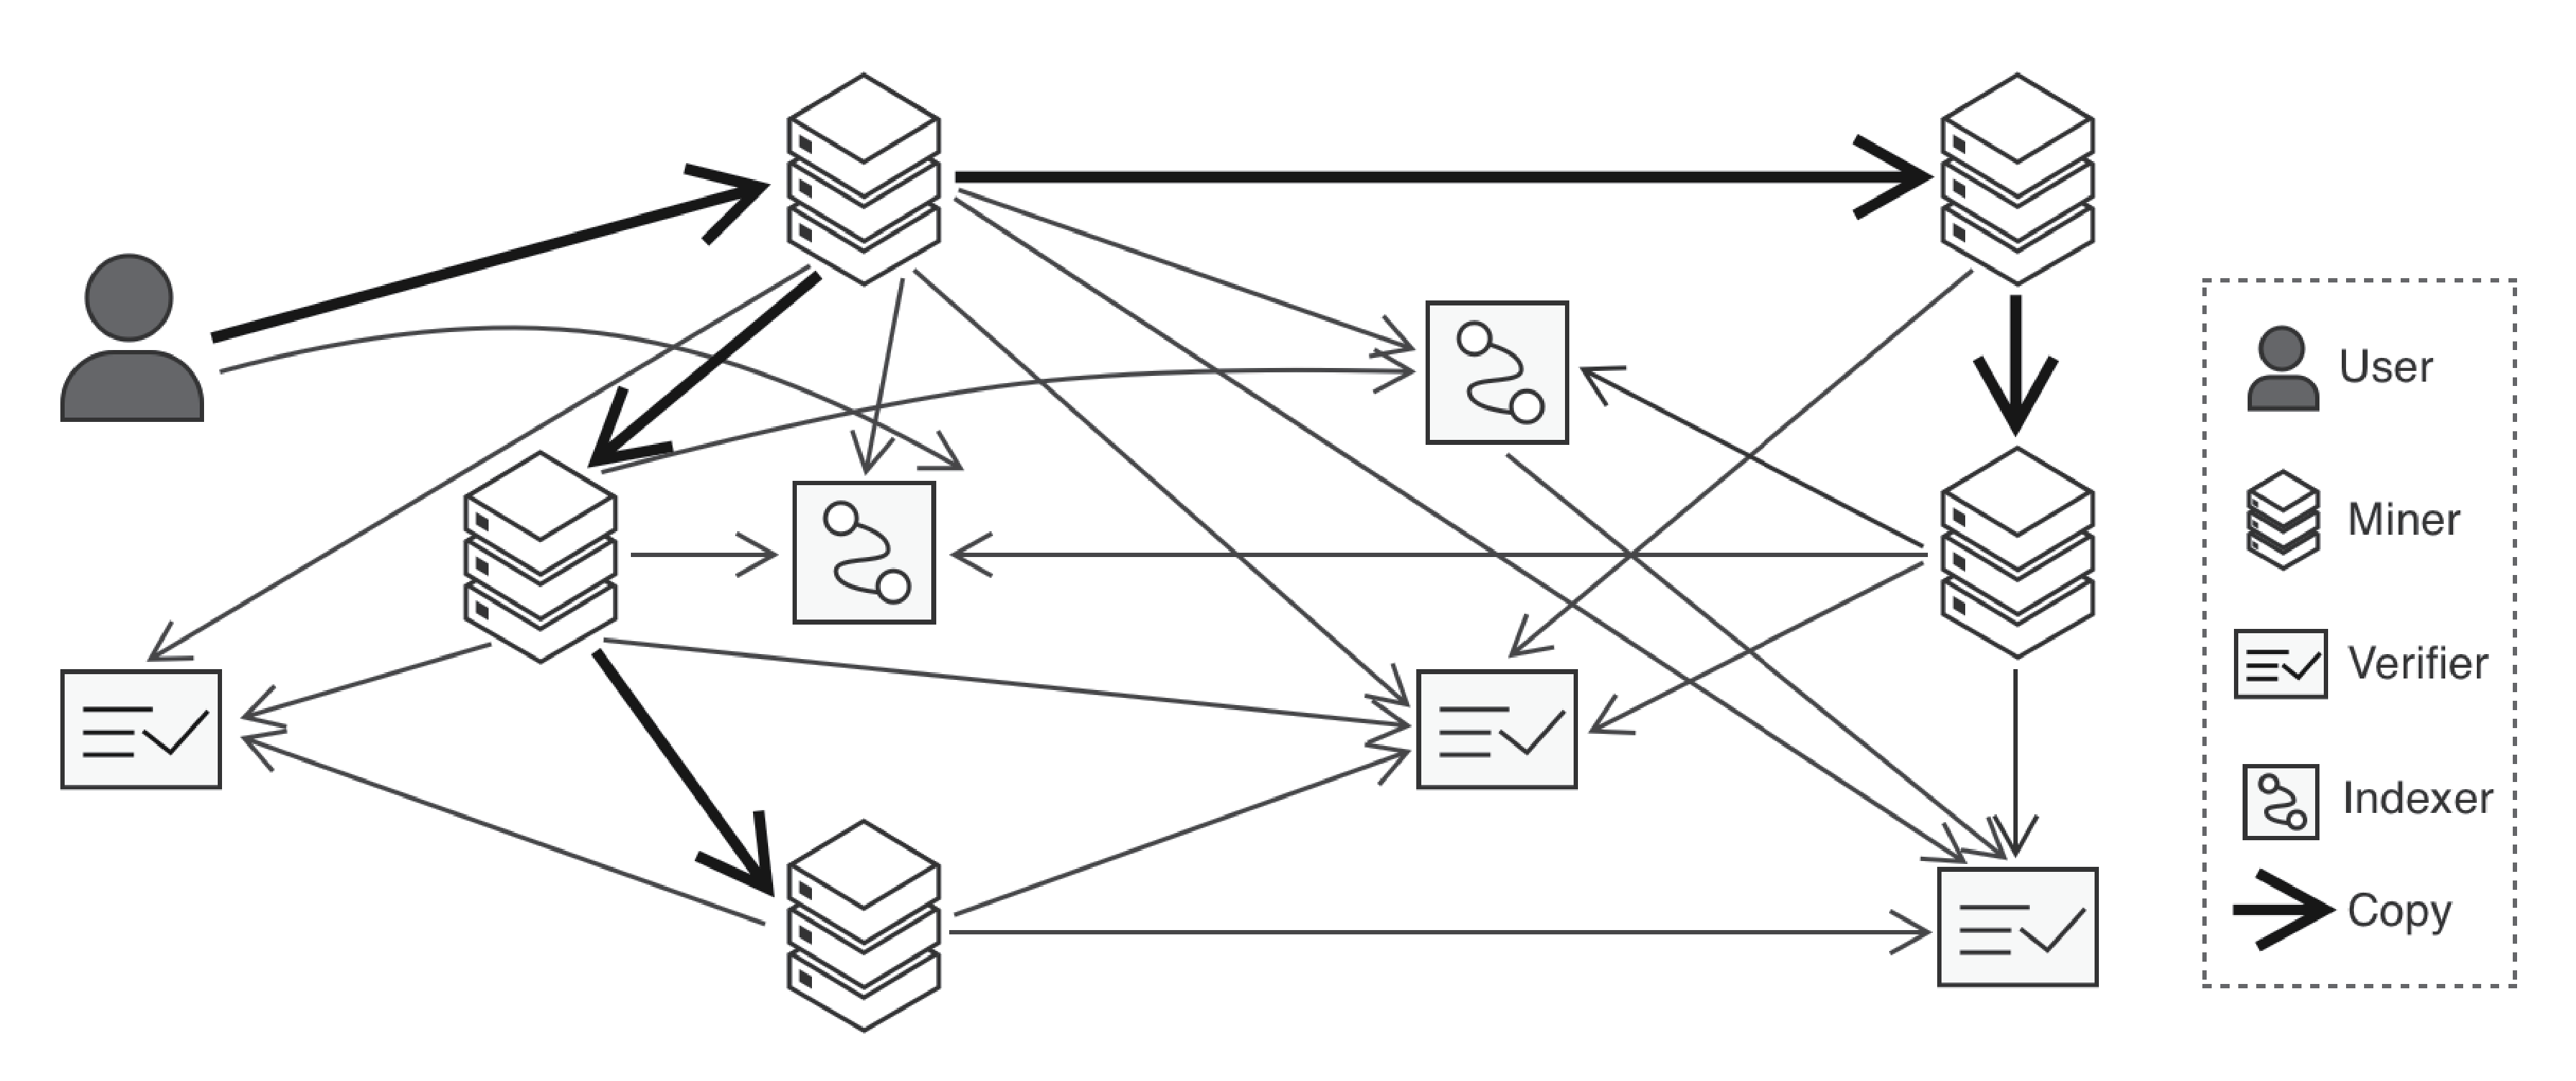
\includegraphics[width=340pt]{fig21}}
\\\\\centerline{{Figure 5.1 Execution of Storage Contract}}%
 \vspace{-1.5em}
\\\\

\noindent   
{\bf Download Contract} 
 \vspace{-0.6em}
\\

\hangafter 1
\hangindent 1.5em
\noindent   
•\quad User pays Gas to download a data object, in the amount of $G_{u}$.
 \vspace{-0.6em}
\\

\hangafter 1
\hangindent 1.5em
\noindent   
•\quad Miner receives Gas for data downloaded from its storage, the more data gets downloaded, the larger the amount of Gas $G_{d}$ it will receive.
 \vspace{-0.6em}
\\

\hangafter 1
\hangindent 1.5em
\noindent   
•\quad Indexer receives Gas for providing scheduling service, in the amount of $G_{index}$.
 \vspace{-0.6em}
\\

\hangafter 1
\hangindent 1.5em
\noindent   
•\quad Verifier receives Gas for conducting Proof of Download (PoD), in the amount of $G_{pod}$.
 \vspace{-0.5em}
\\

\noindent   
The transactions can be formulated as:\\\
 \vspace{-0.5em}
\\\centerline{$G_{u} = \sum G_{d} + \sum G_{pod} + G_{index}$}
%\centerline{$G_{download} = \sum G_{md} + \sum G_{pomd} + G_{index}$}
\\\\ \centerline{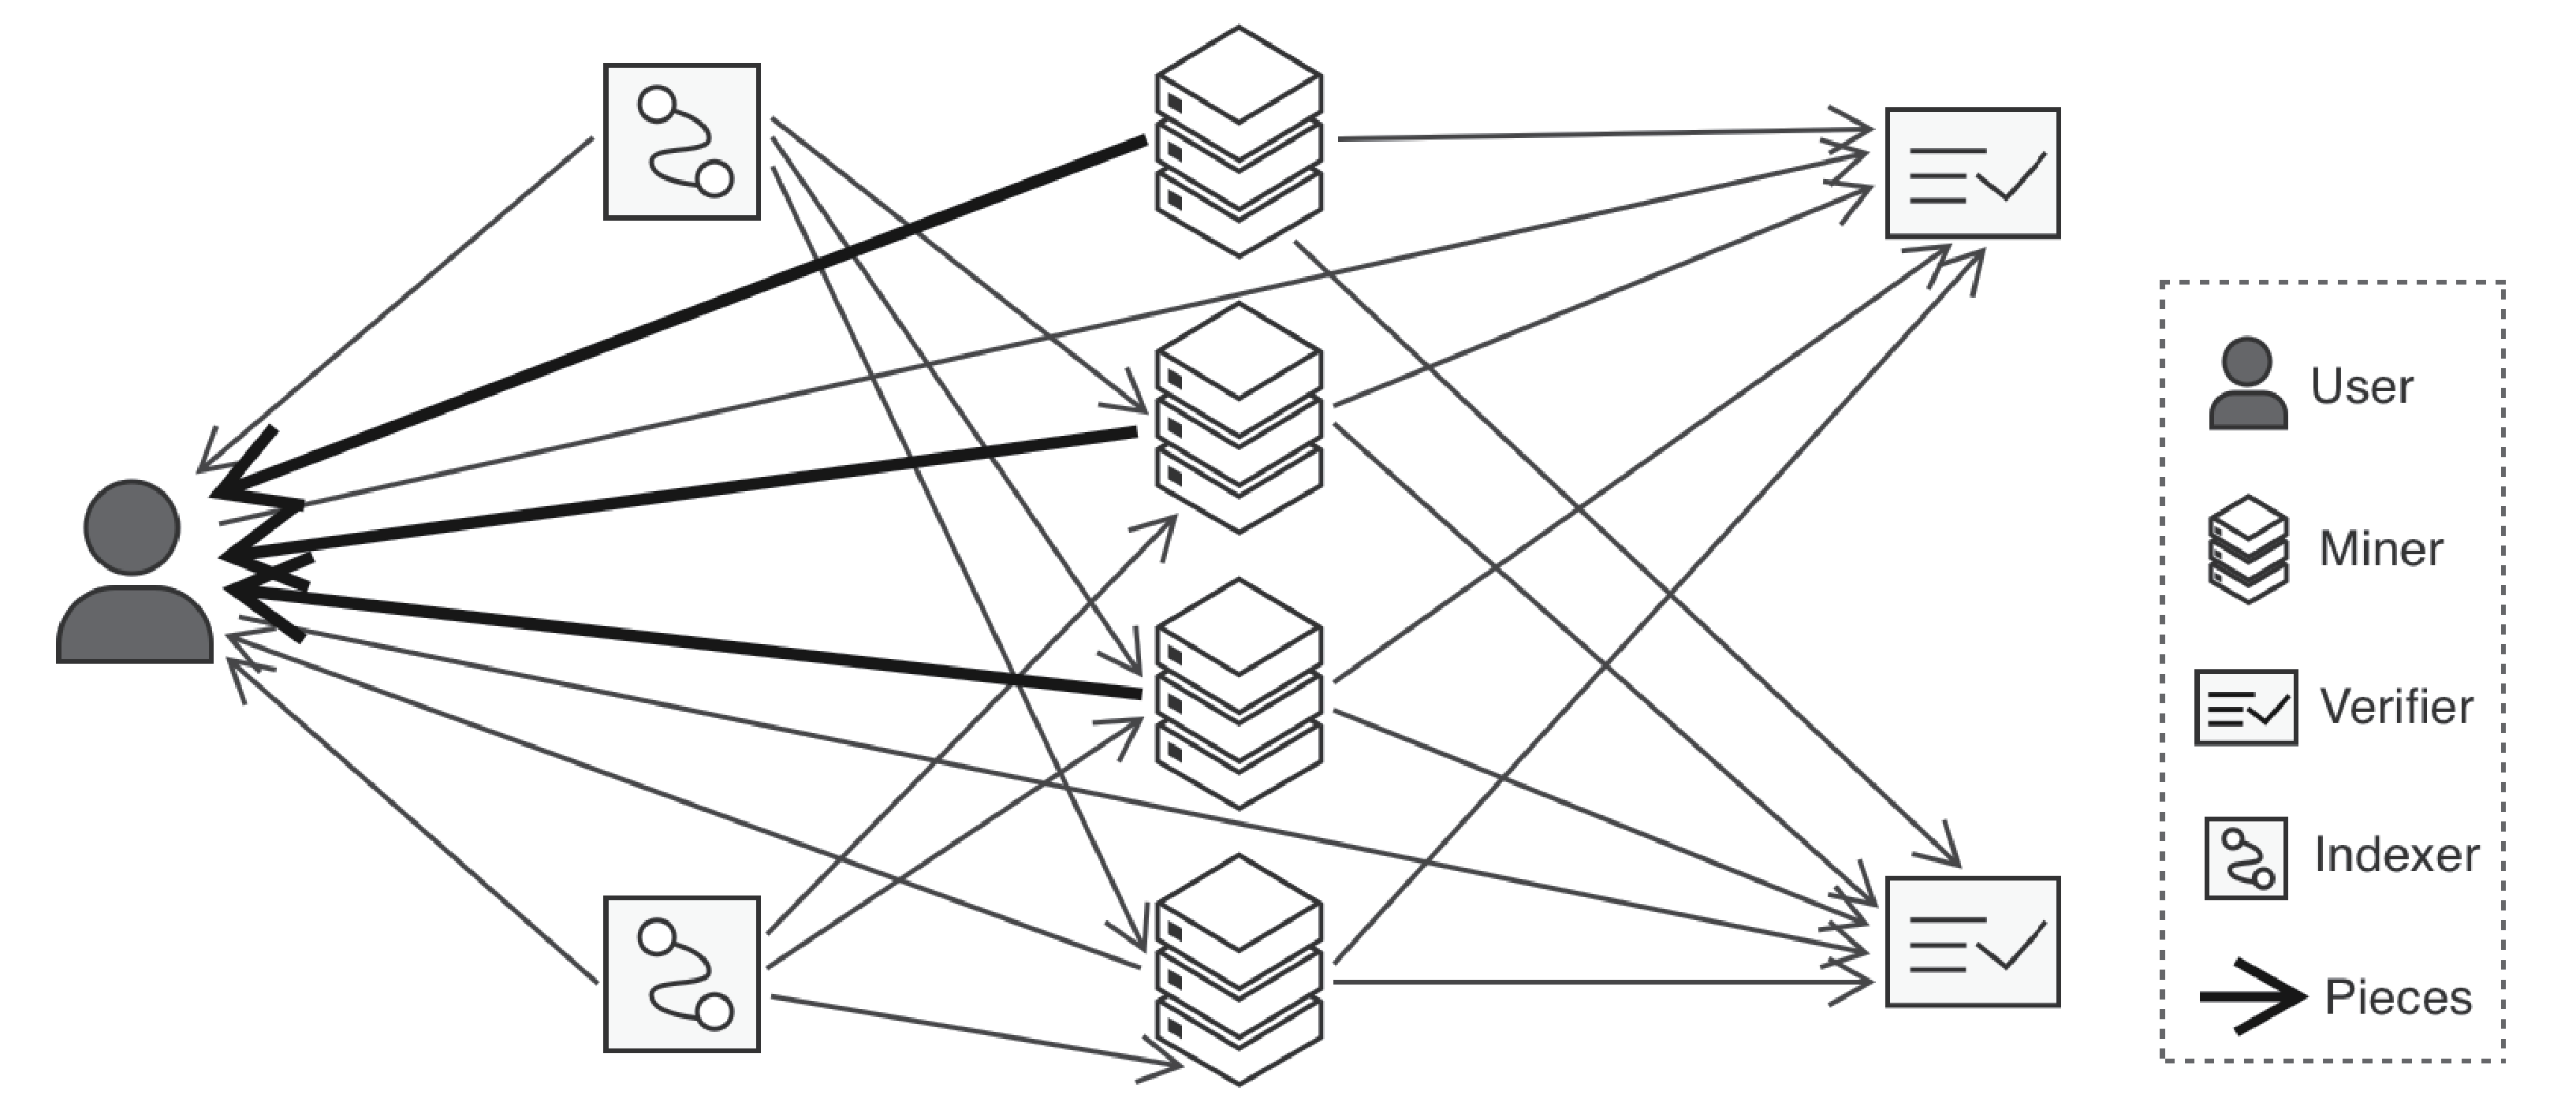
\includegraphics[width=340pt]{fig22}}
\\\\ \centerline{{Figure 5.2 Execution of Download Contract}}%
 \vspace{-0.5em}
\\

\noindent   
User pays PPIO Coins in full up front in these transactions, but the miners receive PPIO Coins gradually as they are providing the service. During the storage period, if a miner goes offline or stops providing the service, the Indexer will find other available miners to store a copy of the data, to maintain the level of data redundancy in the network. At this point, the new miner will start receiving PPIO Coins for storing the copy, while the previous miner will stop receiving further payment.


      \subsection{Gas Price}  %——5.5
The ratio to convert Gas into PPIO Coin is decided by the Gas Price in each contract. The number of PPIO Coins to be paid for a contract is calculated as follows:
 \vspace{-0.5em}
\\ \\ \centerline{$PPIO$ $Coin$$ = GasPrice \cdot Gas$}
 \vspace{-1.5em}
\\ \\$PPIO$ $Coin$ is the number of PPIO Coins that a user is willing to pay when creating the contract. Gas is the total amount of gas units required for executing the contract.
 \vspace{-0.5em}
\\ \\ As discussed in section 5.3, smart contracts can be updated after execution, and new contracts can be created. Every time a contract is created or updated, its Gas Price needs to be decided. The amount of Gas to be spent is decided by the nature of the contract. For example, the gas amount for a storage contract is decided by the size of the data to be stored, the number of copies to be created and the storage period. With the amount of PPIO Coins the user is willing to pay for the contract, its Gas Price can be calculated using the above formula. After the contract is accepted and executed, the total Gas amount is distributed to the nodes involved in executing the contract based on their contribution. Each node will receive the right amount of PPIO Coins calculated using the Gas Price value decided earlier for the contract.
 \vspace{-0.5em}
\\ \\Gas Price is the key for a contract to be accepted in the marketplace. For example, the process of matching a storage contract is to find enough miners that are willing to accept the Gas Price in the contract, so that it can be executed. The higher the Gas Price is, the easier and quicker it is to find enough miners to store the data. Otherwise, if the Gas Price is too low, the contract may never be executed.  
 \vspace{-0.5em}
\\ \\Apart from most other applications, the execution time of a storage contract is usually much longer. For example, the user may store a piece of data for a year. During that time, the price of PPIO Coin could have changed significantly, and such uncertainty increases the risk for both the user and the miner. PPIO adopts a Gas Price Oracle to help reduce the uncertainty, and maintain a more stable and fair economy.
 \vspace{-0.5em}
\\ \\The Oracle calculates and provides a Platform Gas Price. It is expected that at the Platform Gas Price, the majority of the contracts should be able to find a match. The Price is calculated by taking into consideration the transaction history of the entire network, the fluctuation of the PPIO Coin’s price, and the trend of storage and bandwidth cost in the external markets. For example, the cost of storage and bandwidth resources is expected to drop gradually through time, under normal circumstances. Therefore for a storage contract with a prolonged storage period, the Oracle tends to provide lower Platform Gas Price.
 \vspace{-0.5em}
\\\\The Platform Gas Price is a reference price. Each user and miner can decide whether it is an acceptable price for a contract based on their circumstances, and they can propose a different price when needed. As the Oracle takes into account the transactions in the platform, it serves as good guidance and helps stabilize the price in the system.
 \vspace{-0.5em}
\\\\As PPIO is a fully decentralized system, the implementation of Oracle is also decentralized. Multiple nodes in the network can fulfill the functionalities of the Oracle, and the consensus mechanism is also used to ensure its reliability.      
 \vspace{-0.5em}
\subsection{Coin Pool}  %——5.6
Each transaction needs to consume a certain amount of Gas to encourage different nodes in the network to participate. However, if each transaction requires the user to make individual micropayment, the user experience will be degraded, as they need to handle too many payments. Besides, figuring out the right Gas Price for each transaction is also be a burden to most users. Therefore, applications may wish to provide more friendly payment options to the user. For example, a network drive application may wish to provide storage packages that allow the user to make an upfront payment for a specific storage quota for a period (for example, 6 months 200 GB storage). The users don’t need to make additional micropayments for storing or downloading data under these constraints.
 \vspace{-0.5em}
\\ \\PPIO solves this problem by introducing a unique node called {\bf Coin-Pool}. Each Coin-Pool is an individual business entity that is responsible for its profits and losses. Users or developers sign up and purchase services provided by the Coin-Pool, such as storage packages.  Once an agreement is reached, the Coin-Pool will handle all the payments on behalf of the user, when they use any of PPIO’s services that are included in the package they purchased.
 \vspace{-0.5em}
\\
\\\centerline{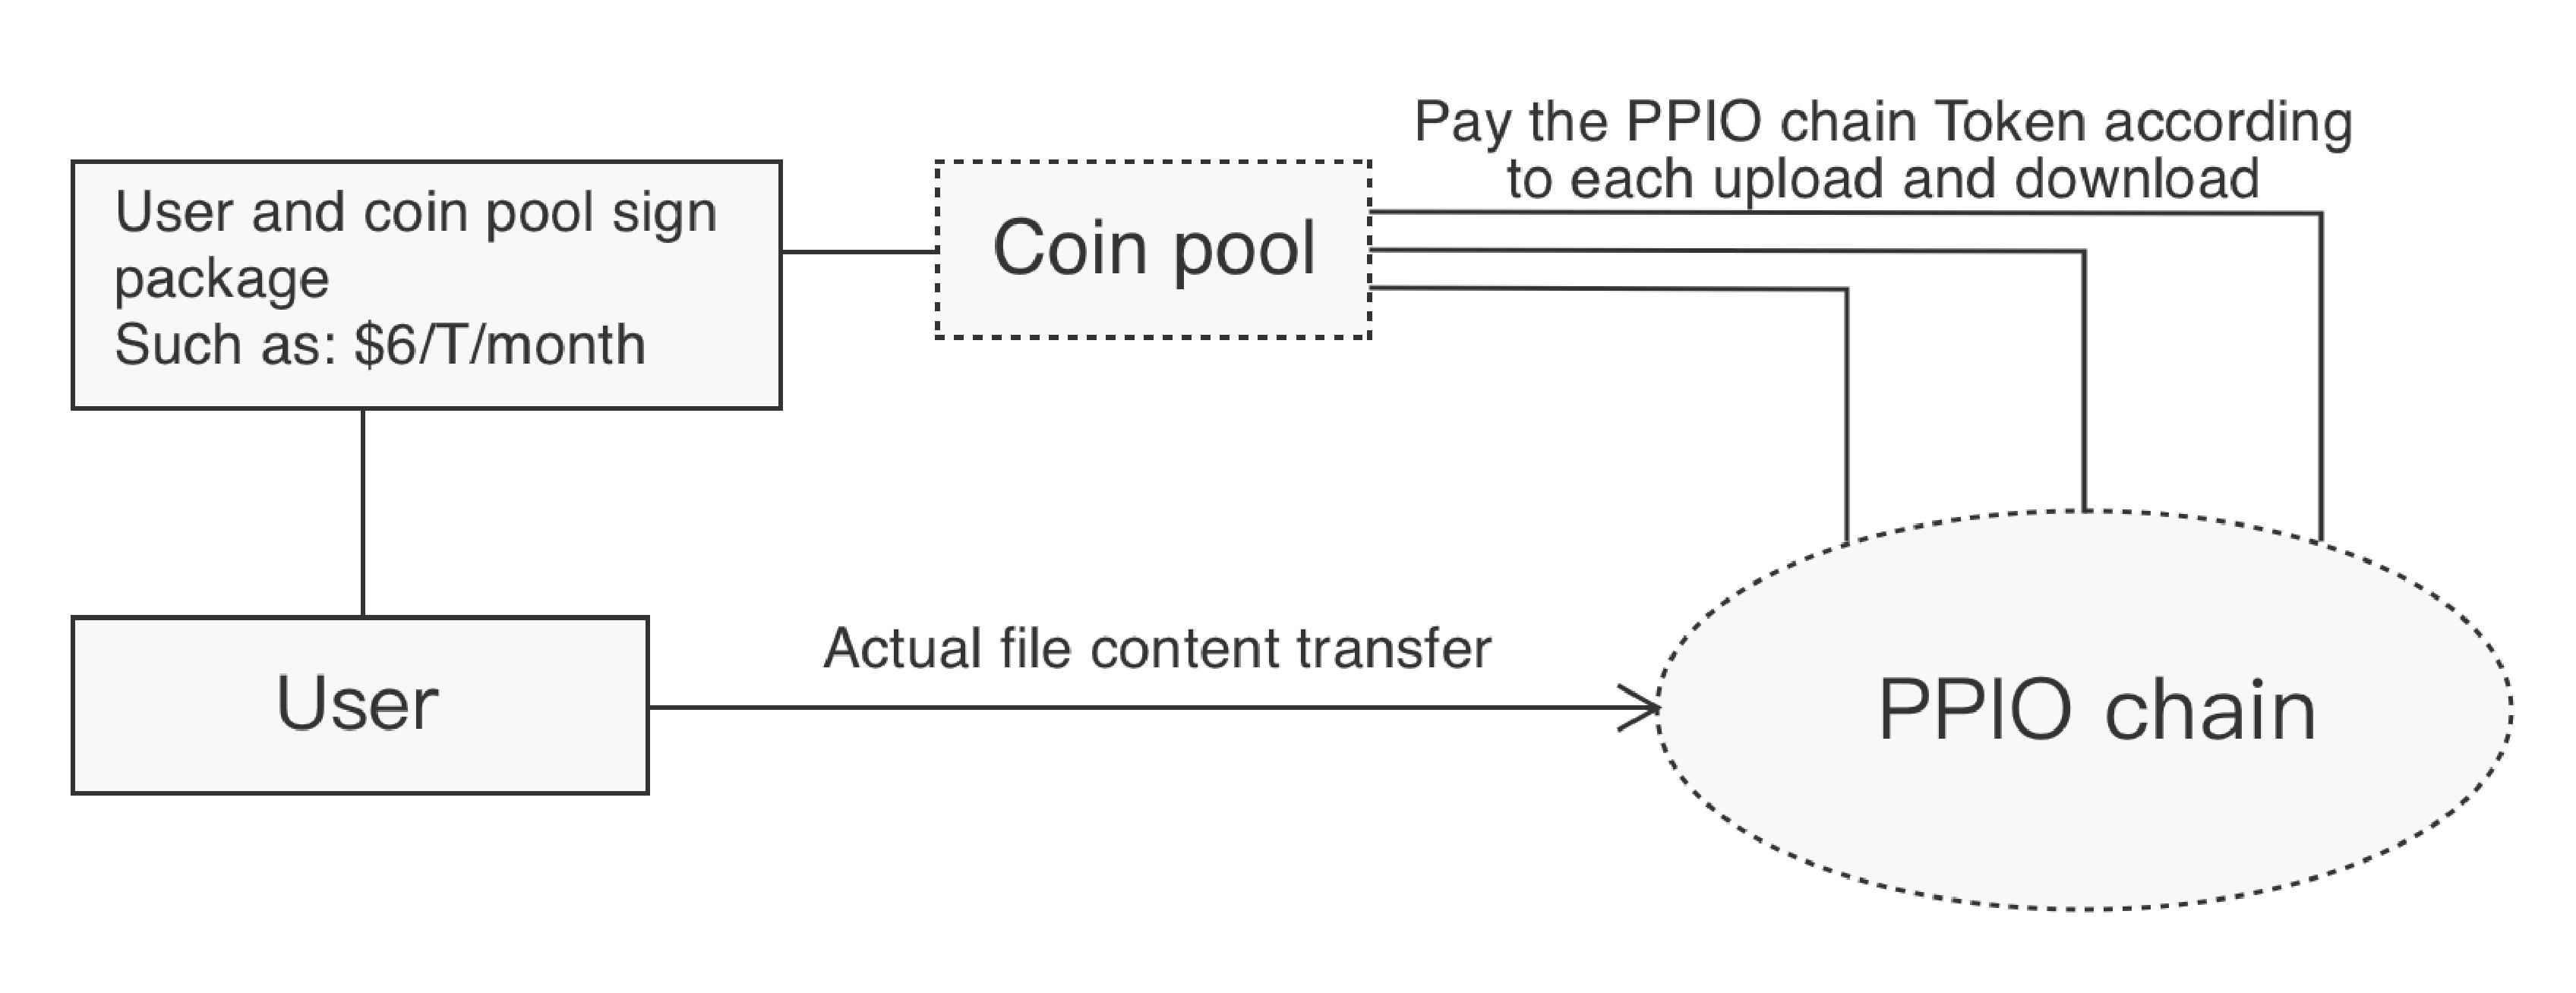
\includegraphics[width=360pt]{fig23}}
\\\centerline{{Figure 5.3 Coin Pool}}%——————————————————————————————待确认名称
 \vspace{-0.5em}
 \\ \\
 {  \bf Coin-Pool has the following characteristics:}
  \vspace{-0.8em}
\\

\hangafter 1
\hangindent 1.8em
\noindent   
1.\quad The users pay the agreed amount of PPIO Coins to the Coin-Pool, when they purchase service packages.
  \vspace{-0.8em}
\\

\hangafter 1
\hangindent 1.8em
\noindent   
2.\quad The Coin-Pool makes payments for each of the user’s transactions in PPIO’s network, based on the agreed service terms. The storage and download operations are still entirely triggered and controlled by the user. 
  \vspace{-0.8em}
\\

\hangafter 1
\hangindent 1.8em
\noindent   
3.\quad To maintain the reliability of such a system, Coin-Pool needs to deposit certain amount of PPIO Coin as a collateral, before it can serve the users. If the Coin-Pool fails to fulfill its agent liability, its deposit can get confiscated. The Coin-Pool may no longer be qualified to provide service, and its existing user and service contracts can be taken over by other qualified Coin-Pools.  
  \vspace{-0.8em}
\\

\hangafter 1
\hangindent 1.8em
\noindent   
4.\quad Necessary information of all Coin-Pools in the network is made public so that users can be informed when choosing a Coin-Pool for themselves. The published information includes the number of PPIO Coins deposited by the Coin-Pool, the total amount of PPIO Coins the Coin-Pool holds for the users, and the number of users signed up for its service.
  \vspace{-0.8em}
\\

\hangafter 1
\hangindent 1.8em
\noindent   
5.\quad PPIO provides a set of APIs to develop a Coin-Pool, to enable the handling of payments for user transactions.
  \vspace{-0.8em}
  \\

\hangafter 1
\hangindent 1.8em
\noindent   
6.\quad Coin-Pool developers can develop payment gateways that allow users to make payments in fiat currency, as well as other cryptocurrencies. It helps make such service accessible by more users.
  \vspace{-0.8em}
\\

\hangafter 1
\hangindent 1.8em
\noindent   
7.\quad Coin-Pool is a business entity that is responsible for its profits and losses. Competition among different Coin-Pools can make the price more affordable by the users, and help maintain a healthier overall economy in PPIO’s storage network.
  \vspace{-0.5em}

   \section{Future} %——7

\hangafter 1
\hangindent 1.5em
\noindent   
•\quad  {\bf Hot storage and cold storage ratings} 
  \vspace{-0.6em}
\\ \\Storage contents are generally categorized under Hot Storage and Cold Storage. Hot storage is data you need to access right away, where performance is at the premium (such as news sites); Cold storage is information that you do not need to access very often. Inactive data do not need to be accessed for a long period is the sort of content that cold storage is ideal for (such as data storage). These two conditions are different regarding storage and network bandwidth efficiency. We are likely to implement two different designs in the future for storage solutions in our ecosystem to make better use of storage space and bandwidth;
  \vspace{-0.6em}
\\

\hangafter 1
\hangindent 1.5em
\noindent   
•\quad  {\bf VCDN Acceleration} 
  \vspace{-0.6em}
\\ \\For use case such as live video streaming that requires massive content delivery acceleration, nodes with high-quality bandwidths are preferred over storage capacities. We will introduce a set of PCDN acceleration designs to utilize bandwidth resources for such needs. The solution will bring higher revenues for nodes that have depleted all their storage resources while meeting the demand for increased bandwidths;
  \vspace{-0.6em}
\\

\hangafter 1
\hangindent 1.5em
\noindent   
•\quad  {\bf More ideas} 
  \vspace{-0.6em}
\\ \\When an ecosystem is formed from the transactions between storage supply and demand, we believe a storage-based value network is created. Price evaluations are made open and transparent on the network for each file downloaded or accessed, in a manner the ecosystem helps quantify each content value associated. It signifies the coming era of a value network. PPIO ultimately provides a system of big data for the most secure and protected storage solutions for all top applications and innovations, bring AI closer, and build a smarter and better future for all of us.

    \newpage    
    \section{REFERENCES} %——11     
  \renewcommand\refname

\begin{thebibliography}{99} 
  \vspace{-1.5em}
\bibitem{article1} M. Piatek, A. Krishnamurthy, A. Venkataramani, R. Yang, D. Zhang and A. Jaffe, "Contracts: Practical Contribution Incentives for P2P Live Streaming"
  \vspace{-1em}
\\

\hangafter 1
\hangindent 1.5em
\noindent  
\bibitem{article2} J. Benet, D. Dalrymple, and N. Greco. Proof of replication. Technical report, Protocol Labs, July 27,2017. https://filecoin.io/proof-of-replication.pdf Accessed June 2018.
  \vspace{-1em}
\\

\hangafter 1
\hangindent 1.5em
\noindent  
\bibitem{article3} S. Dziembowski, S. Faust, V. Kolmogorov, K. Pietrzak, "Proofs of Space".
  \vspace{-1em}
\\

\hangafter 1
\hangindent 1.5em
\noindent  
\bibitem{article4} Yan Huang, Tom Z.J. Fu, Dah-Ming Gao, John C.S. Lui, Cheng Huang, "Challenges, design and analysis of a large-scale p2p-vod system",ACM Sigcomm 2008.
  \vspace{-1em}
\\

\hangafter 1
\hangindent 1.5em
\noindent  
\bibitem{article5} XU Ke, Haitao Li, Jiangchuan Liu, Wei Zhu, Wenyu Wang, "PPVA: A Universal and Transparent Peer-to-Peer Accelerator for Interactive Online Video Sharing," IEEE IWQoS 2010.
  \vspace{-1em}
\\

\hangafter 1
\hangindent 1.5em
\noindent  
\bibitem{article6} Huang Yan, Xu Ke., Li HaiTao, Cao Yang, Yao Xin, "Large-scale P2PVOD system: Focusing on clients".
  \vspace{-1em}
\\

\hangafter 1
\hangindent 1.5em
\noindent  
\bibitem{article7}Li Haitao, Ke Xu, James Seng, Po Hu, "Towards health of replication in large-scale P2P-VoD systems," IEEE IPCCC 2009.
  \vspace{-1em}
\\

\hangafter 1
\hangindent 1.5em
\noindent  
\bibitem{article8} https://github.com/skywind3000/kcp/blob/master/protocol.txt 2018.
  \vspace{-1em}
\\

\hangafter 1
\hangindent 1.5em
\noindent  
\bibitem{article9}R. Hamilton, J. Iyengar, I. Swett, A. Wilk, "QUIC: A UDP-Based Secure and Reliable Transport for HTTP/2" IETF:draft-tsvwg-quic-protocol 2016.
  \vspace{-1em}
\\

\hangafter 1
\hangindent 1.5em
\noindent  
\bibitem{article10} R. R. Stewart and Q. Xie. Stream control transmission protocol (SCTP): a reference guide. Addison-Wesley Longman Publishing Co., Inc., 2001.
  \vspace{-1em}
\\

\hangafter 1
\hangindent 1.5em
\noindent  
\bibitem{article11}Mirrokni, Vahab, Mikkel Thorup, and Morteza Zadimoghaddam. "Consistent Hashing with Bounded Loads." arXiv:1608.01350(2016).
  \vspace{-1em}
\\

\hangafter 1
\hangindent 1.5em
\noindent  
\bibitem{article12}Xinyan Zhang, Jiangchuan Liu, Bo Liz, and Tak-Shing Peter Yum, "CoolStreaming/DONet: A Data-Driven Overlay Network for Efficient Live Media Streaming".
  \vspace{-1em}
\\

\hangafter 1
\hangindent 1.5em
\noindent  
\bibitem{article13}Yunhong Gu, Robert L.Grossma, "UDT: UDP-based data transfer for high-speed wide area networks".
  \vspace{-1em}
\\

\hangafter 1
\hangindent 1.5em
\noindent  
\bibitem{article14}Stoica, I., Morris, R., Karger, D., Kaashoek, M. F. and Balakrishnan, H., "Chord: A scalable peer-to-peer lookup service for internet applications". ACM SIGCOMM Computer Communication Review. 31(4), 149.
  \vspace{-1em}
\\

\hangafter 1
\hangindent 1.5em
\noindent  
\bibitem{article15} Rowstron, A. and Druschel, P, "Pastry: Scalable, decentralized object location and routing for large-scale peer-to-peer systems". IFIP/ACM International Conference on Distributed Systems Platforms (Middleware), Heidelberg, Germany.
  \vspace{-1em}
\\

\hangafter 1
\hangindent 1.5em
\noindent  
\bibitem{article16}Petar Maymounkov, David Mazieres, "Kademlia: a peer-to-peer information system based on the XOR metric, International Workshop on Peer-to-Peer Systems".
  \vspace{-1em}
\\

\hangafter 1
\hangindent 1.5em
\noindent  
\bibitem{article17} Haiyong Xie, Y. Richard Yang, Arvind Krishnamurthy, Yanbin Liu§ Avi Silberschatz, "P4P: Provider Portal for Applications", ACM SIGCOMM 2008.
  \vspace{-1em}
\\

\hangafter 1
\hangindent 1.5em
\noindent  
\bibitem{article18}Zhao, Ben Yanbin, John Kubiatowicz, and Anthony D. Joseph. "Tapestry: An infrastructure for fault-tolerant wide-area locationand routing." (2001): 70.
  \vspace{-1em}
\\

\hangafter 1
\hangindent 1.5em
\noindent  
\bibitem{article19} DeCandia, Giuseppe, et al. "Dynamo: amazon's highly available key-value store." ACM SIGOPS operating systems review. Vol. 41. No. 6. ACM, 2007.“
  \vspace{-1em}
\\

\hangafter 1
\hangindent 1.5em
\noindent  
\bibitem{article20} Micali, Silvio; Rabin, Michael O.; Vadhan, Salil P. (1999). "Verifiable random functions". Proceedings of the 40th IEEE Symposium on Foundations of Computer Science. pp. 120–130.
  \vspace{-1em}
\\

\hangafter 1
\hangindent 1.5em
\noindent  
\bibitem{article21} L. Lamport, R. Shostak, M. Pease, “The Byzantine Generals Problem”, TPLS 4(3), 1982.
  \vspace{-1em}
\\

\hangafter 1
\hangindent 1.5em
\noindent  
\bibitem{article22}$ https://en.wikipedia.org/wiki/Reed\%E2\%80\%93Solomon_error_correction$.
  \vspace{-1em}
\\

\hangafter 1
\hangindent 1.5em
\noindent  
\bibitem{article23}  I. Baumgart and S. Mies. S/kademlia: A practicable approach towards secure key-based routing. In Parallel and Distributed Systems, 2007 International.
  \vspace{-1em}
\\

\hangafter 1
\hangindent 1.5em
\noindent  
\bibitem{article24} Verifiable Random Funciton, Wikipedia, $https://en.wikipedia.org/wiki/Verifiable_random_function$.
  \vspace{-1em}
\\

\hangafter 1
\hangindent 1.5em
\noindent  
\bibitem{article25}Yevgeniy Dodis and Aleksandr Yampolskiy. "A verifiable random function with short proofs and keys." In Public Key Cryptography, pages 416–431, 2005.
  \vspace{-1em}
\\

\hangafter 1
\hangindent 1.5em
\noindent  
\bibitem{article26}xfiPogue Internet Study 2007,$ https://www.ipoque.com/news-media/press-releases/2007/ipoque-internet-study-2007-p2p-file-sharing-still-dominates$.

\end{thebibliography}

   
\end{document}